\documentclass[twoside]{book}

% Packages required by doxygen
\usepackage{fixltx2e}
\usepackage{calc}
\usepackage{doxygen}
\usepackage[export]{adjustbox} % also loads graphicx
\usepackage{graphicx}
\usepackage[utf8]{inputenc}
\usepackage{makeidx}
\usepackage{multicol}
\usepackage{multirow}
\PassOptionsToPackage{warn}{textcomp}
\usepackage{textcomp}
\usepackage[nointegrals]{wasysym}
\usepackage[table]{xcolor}

% NLS support packages
\usepackage[ngerman]{babel}

% Font selection
\usepackage[T1]{fontenc}
\usepackage[scaled=.90]{helvet}
\usepackage{courier}
\usepackage{amssymb}
\usepackage{sectsty}
\renewcommand{\familydefault}{\sfdefault}
\allsectionsfont{%
  \fontseries{bc}\selectfont%
  \color{darkgray}%
}
\renewcommand{\DoxyLabelFont}{%
  \fontseries{bc}\selectfont%
  \color{darkgray}%
}
\newcommand{\+}{\discretionary{\mbox{\scriptsize$\hookleftarrow$}}{}{}}

% Page & text layout
\usepackage{geometry}
\geometry{%
  a4paper,%
  top=2.5cm,%
  bottom=2.5cm,%
  left=2.5cm,%
  right=2.5cm%
}
\tolerance=750
\hfuzz=15pt
\hbadness=750
\setlength{\emergencystretch}{15pt}
\setlength{\parindent}{0cm}
\setlength{\parskip}{3ex plus 2ex minus 2ex}
\makeatletter
\renewcommand{\paragraph}{%
  \@startsection{paragraph}{4}{0ex}{-1.0ex}{1.0ex}{%
    \normalfont\normalsize\bfseries\SS@parafont%
  }%
}
\renewcommand{\subparagraph}{%
  \@startsection{subparagraph}{5}{0ex}{-1.0ex}{1.0ex}{%
    \normalfont\normalsize\bfseries\SS@subparafont%
  }%
}
\makeatother

% Headers & footers
\usepackage{fancyhdr}
\pagestyle{fancyplain}
\fancyhead[LE]{\fancyplain{}{\bfseries\thepage}}
\fancyhead[CE]{\fancyplain{}{}}
\fancyhead[RE]{\fancyplain{}{\bfseries\leftmark}}
\fancyhead[LO]{\fancyplain{}{\bfseries\rightmark}}
\fancyhead[CO]{\fancyplain{}{}}
\fancyhead[RO]{\fancyplain{}{\bfseries\thepage}}
\fancyfoot[LE]{\fancyplain{}{}}
\fancyfoot[CE]{\fancyplain{}{}}
\fancyfoot[RE]{\fancyplain{}{\bfseries\scriptsize Erzeugt von Doxygen }}
\fancyfoot[LO]{\fancyplain{}{\bfseries\scriptsize Erzeugt von Doxygen }}
\fancyfoot[CO]{\fancyplain{}{}}
\fancyfoot[RO]{\fancyplain{}{}}
\renewcommand{\footrulewidth}{0.4pt}
\renewcommand{\chaptermark}[1]{%
  \markboth{#1}{}%
}
\renewcommand{\sectionmark}[1]{%
  \markright{\thesection\ #1}%
}

% Indices & bibliography
\usepackage{natbib}
\usepackage[titles]{tocloft}
\setcounter{tocdepth}{3}
\setcounter{secnumdepth}{5}
\makeindex

% Hyperlinks (required, but should be loaded last)
\usepackage{ifpdf}
\ifpdf
  \usepackage[pdftex,pagebackref=true]{hyperref}
\else
  \usepackage[ps2pdf,pagebackref=true]{hyperref}
\fi
\hypersetup{%
  colorlinks=true,%
  linkcolor=blue,%
  citecolor=blue,%
  unicode%
}

% Custom commands
\newcommand{\clearemptydoublepage}{%
  \newpage{\pagestyle{empty}\cleardoublepage}%
}

\usepackage{caption}
\captionsetup{labelsep=space,justification=centering,font={bf},singlelinecheck=off,skip=4pt,position=top}

%===== C O N T E N T S =====

\begin{document}

% Titlepage & ToC
\hypersetup{pageanchor=false,
             bookmarksnumbered=true,
             pdfencoding=unicode
            }
\pagenumbering{alph}
\begin{titlepage}
\vspace*{7cm}
\begin{center}%
{\Large Übung Objektorientierte Programmierung \\[1ex]\large 1.\+0 }\\
\vspace*{1cm}
{\large Erzeugt von Doxygen 1.8.13}\\
\end{center}
\end{titlepage}
\clearemptydoublepage
\pagenumbering{roman}
\tableofcontents
\clearemptydoublepage
\pagenumbering{arabic}
\hypersetup{pageanchor=true}

%--- Begin generated contents ---
\chapter{Hierarchie-\/\+Verzeichnis}
\section{Klassenhierarchie}
Die Liste der Ableitungen ist -\/mit Einschränkungen-\/ alphabetisch sortiert\+:\begin{DoxyCompactList}
\item \contentsline{section}{C\+Counter}{\pageref{class_c_counter}}{}
\begin{DoxyCompactList}
\item \contentsline{section}{C\+Forward\+Counter}{\pageref{class_c_forward_counter}}{}
\item \contentsline{section}{C\+Variable\+Counter}{\pageref{class_c_variable_counter}}{}
\end{DoxyCompactList}
\end{DoxyCompactList}

\chapter{Klassen-\/\+Verzeichnis}
\section{Auflistung der Klassen}
Hier folgt die Aufzählung aller Klassen, Strukturen, Varianten und Schnittstellen mit einer Kurzbeschreibung\+:\begin{DoxyCompactList}
\item\contentsline{section}{\hyperlink{class_c_counter}{C\+Counter} }{\pageref{class_c_counter}}{}
\item\contentsline{section}{\hyperlink{class_c_forward_counter}{C\+Forward\+Counter} }{\pageref{class_c_forward_counter}}{}
\item\contentsline{section}{\hyperlink{class_c_variable_counter}{C\+Variable\+Counter} }{\pageref{class_c_variable_counter}}{}
\end{DoxyCompactList}

\chapter{Datei-\/\+Verzeichnis}
\section{Auflistung der Dateien}
Hier folgt die Aufzählung aller Dateien mit einer Kurzbeschreibung\+:\begin{DoxyCompactList}
\item\contentsline{section}{C\+:/portable\+Dev\+Env\+\_\+2017/workspace2017/project/src/\hyperlink{_c_array_8hpp}{C\+Array.\+hpp} \\*Template-\/\+Klasse \hyperlink{class_c_array}{C\+Array} Erzeugt ein Array vom Typ T mit N Elementen }{\pageref{_c_array_8hpp}}{}
\item\contentsline{section}{C\+:/portable\+Dev\+Env\+\_\+2017/workspace2017/project/src/\hyperlink{_c_array_dec_8cpp}{C\+Array\+Dec.\+cpp} \\*Created on\+: 24.\+05.\+2018 Author\+: diamo }{\pageref{_c_array_dec_8cpp}}{}
\item\contentsline{section}{C\+:/portable\+Dev\+Env\+\_\+2017/workspace2017/project/src/\hyperlink{_c_array_dec_8hpp}{C\+Array\+Dec.\+hpp} \\*L\+ZW Decoder, Dictionary implementiert als Array }{\pageref{_c_array_dec_8hpp}}{}
\item\contentsline{section}{C\+:/portable\+Dev\+Env\+\_\+2017/workspace2017/project/src/\hyperlink{_c_array_enc_8cpp}{C\+Array\+Enc.\+cpp} \\*Created on\+: 24.\+05.\+2018 Author\+: diamo }{\pageref{_c_array_enc_8cpp}}{}
\item\contentsline{section}{C\+:/portable\+Dev\+Env\+\_\+2017/workspace2017/project/src/\hyperlink{_c_array_enc_8hpp}{C\+Array\+Enc.\+hpp} \\*L\+ZW Encoder, Dictionary implementiert als Array }{\pageref{_c_array_enc_8hpp}}{}
\item\contentsline{section}{C\+:/portable\+Dev\+Env\+\_\+2017/workspace2017/project/src/\hyperlink{_c_counter_8cpp}{C\+Counter.\+cpp} \\*Created on\+: 06.\+04.\+2018 Author\+: diamo }{\pageref{_c_counter_8cpp}}{}
\item\contentsline{section}{C\+:/portable\+Dev\+Env\+\_\+2017/workspace2017/project/src/\hyperlink{_c_counter_8hpp}{C\+Counter.\+hpp} \\*Created on\+: 06.\+04.\+2018 Author\+: diamo }{\pageref{_c_counter_8hpp}}{}
\item\contentsline{section}{C\+:/portable\+Dev\+Env\+\_\+2017/workspace2017/project/src/\hyperlink{_c_dec_8cpp}{C\+Dec.\+cpp} }{\pageref{_c_dec_8cpp}}{}
\item\contentsline{section}{C\+:/portable\+Dev\+Env\+\_\+2017/workspace2017/project/src/\hyperlink{_c_dec_8hpp}{C\+Dec.\+hpp} \\*Klasse \hyperlink{class_c_dec}{C\+Dec} Abstrakte Basisklasse für Decodierung }{\pageref{_c_dec_8hpp}}{}
\item\contentsline{section}{C\+:/portable\+Dev\+Env\+\_\+2017/workspace2017/project/src/\hyperlink{_c_double_hashing_8cpp}{C\+Double\+Hashing.\+cpp} \\*Created on\+: 18.\+05.\+2018 Author\+: diamo }{\pageref{_c_double_hashing_8cpp}}{}
\item\contentsline{section}{C\+:/portable\+Dev\+Env\+\_\+2017/workspace2017/project/src/\hyperlink{_c_double_hashing_8hpp}{C\+Double\+Hashing.\+hpp} \\*Klasse zum Hashen }{\pageref{_c_double_hashing_8hpp}}{}
\item\contentsline{section}{C\+:/portable\+Dev\+Env\+\_\+2017/workspace2017/project/src/\hyperlink{_c_enc_8cpp}{C\+Enc.\+cpp} }{\pageref{_c_enc_8cpp}}{}
\item\contentsline{section}{C\+:/portable\+Dev\+Env\+\_\+2017/workspace2017/project/src/\hyperlink{_c_enc_8hpp}{C\+Enc.\+hpp} \\*Klasse \hyperlink{class_c_enc}{C\+Enc} Abstrakte Basisklasse für Encodierung }{\pageref{_c_enc_8hpp}}{}
\item\contentsline{section}{C\+:/portable\+Dev\+Env\+\_\+2017/workspace2017/project/src/\hyperlink{_c_entry_8cpp}{C\+Entry.\+cpp} \\*Created on\+: 21.\+04.\+2018 Author\+: diamo }{\pageref{_c_entry_8cpp}}{}
\item\contentsline{section}{C\+:/portable\+Dev\+Env\+\_\+2017/workspace2017/project/src/\hyperlink{_c_entry_8hpp}{C\+Entry.\+hpp} \\*Enthält die Basisklasse \hyperlink{class_c_entry}{C\+Entry} Wird später von \hyperlink{class_c_knot}{C\+Knot} benötigt }{\pageref{_c_entry_8hpp}}{}
\item\contentsline{section}{C\+:/portable\+Dev\+Env\+\_\+2017/workspace2017/project/src/\hyperlink{_c_forward_counter_8cpp}{C\+Forward\+Counter.\+cpp} \\*Created on\+: 07.\+04.\+2018 Author\+: diamo }{\pageref{_c_forward_counter_8cpp}}{}
\item\contentsline{section}{C\+:/portable\+Dev\+Env\+\_\+2017/workspace2017/project/src/\hyperlink{_c_forward_counter_8hpp}{C\+Forward\+Counter.\+hpp} \\*Created on\+: 07.\+04.\+2018 Author\+: diamo }{\pageref{_c_forward_counter_8hpp}}{}
\item\contentsline{section}{C\+:/portable\+Dev\+Env\+\_\+2017/workspace2017/project/src/\hyperlink{_c_knot_8cpp}{C\+Knot.\+cpp} \\*Created on\+: 11.\+05.\+2018 Author\+: diamo }{\pageref{_c_knot_8cpp}}{}
\item\contentsline{section}{C\+:/portable\+Dev\+Env\+\_\+2017/workspace2017/project/src/\hyperlink{_c_knot_8hpp}{C\+Knot.\+hpp} \\*Enthält die Klasse \hyperlink{class_c_entry}{C\+Entry} Erbt von \hyperlink{class_c_knot}{C\+Knot} }{\pageref{_c_knot_8hpp}}{}
\item\contentsline{section}{C\+:/portable\+Dev\+Env\+\_\+2017/workspace2017/project/src/\hyperlink{_c_l_z_w_8cpp}{C\+L\+Z\+W.\+cpp} }{\pageref{_c_l_z_w_8cpp}}{}
\item\contentsline{section}{C\+:/portable\+Dev\+Env\+\_\+2017/workspace2017/project/src/\hyperlink{_c_l_z_w_8hpp}{C\+L\+Z\+W.\+hpp} \\*\hyperlink{_c_l_z_w_8hpp}{C\+L\+Z\+W.\+hpp} Basisklasse für L\+ZW Encoder und Decoder }{\pageref{_c_l_z_w_8hpp}}{}
\item\contentsline{section}{C\+:/portable\+Dev\+Env\+\_\+2017/workspace2017/project/src/\hyperlink{_c_trie_dec_8cpp}{C\+Trie\+Dec.\+cpp} \\*Created on\+: 29.\+05.\+2018 Author\+: diamo }{\pageref{_c_trie_dec_8cpp}}{}
\item\contentsline{section}{C\+:/portable\+Dev\+Env\+\_\+2017/workspace2017/project/src/\hyperlink{_c_trie_dec_8hpp}{C\+Trie\+Dec.\+hpp} \\*L\+ZW Decoder, Dictionary implementiert als Trie }{\pageref{_c_trie_dec_8hpp}}{}
\item\contentsline{section}{C\+:/portable\+Dev\+Env\+\_\+2017/workspace2017/project/src/\hyperlink{_c_trie_enc_8cpp}{C\+Trie\+Enc.\+cpp} \\*Created on\+: 29.\+05.\+2018 Author\+: diamo }{\pageref{_c_trie_enc_8cpp}}{}
\item\contentsline{section}{C\+:/portable\+Dev\+Env\+\_\+2017/workspace2017/project/src/\hyperlink{_c_trie_enc_8hpp}{C\+Trie\+Enc.\+hpp} \\*L\+ZW Encoder, Dictionary implementiert als Trie }{\pageref{_c_trie_enc_8hpp}}{}
\item\contentsline{section}{C\+:/portable\+Dev\+Env\+\_\+2017/workspace2017/project/src/\hyperlink{main_praktikum_8cpp}{main\+Praktikum.\+cpp} }{\pageref{main_praktikum_8cpp}}{}
\item\contentsline{section}{C\+:/portable\+Dev\+Env\+\_\+2017/workspace2017/project/src/\hyperlink{_x_out_of_bounds_8cpp}{X\+Out\+Of\+Bounds.\+cpp} \\*Created on\+: 10.\+05.\+2018 Author\+: diamo }{\pageref{_x_out_of_bounds_8cpp}}{}
\item\contentsline{section}{C\+:/portable\+Dev\+Env\+\_\+2017/workspace2017/project/src/\hyperlink{_x_out_of_bounds_8hpp}{X\+Out\+Of\+Bounds.\+hpp} \\*Enthält die Klasse \hyperlink{class_x_out_of_bounds}{X\+Out\+Of\+Bounds} Es handelt sich hierbei um eine Klasse die Ausnahmeobjekte erstellt }{\pageref{_x_out_of_bounds_8hpp}}{}
\end{DoxyCompactList}

\chapter{Klassen-\/\+Dokumentation}
\hypertarget{class_c_array}{}\section{C\+Array$<$ T, N $>$ Template-\/\+Klassenreferenz}
\label{class_c_array}\index{C\+Array$<$ T, N $>$@{C\+Array$<$ T, N $>$}}


Erzeugt ein Array vom Typ T mit N Elementen Es existiert ein Kopierkonstruktor, der eine tiefe Kopie eines anderen Objekts gleichen Typs erzeugt. Mithilfe des operators \mbox{[}\mbox{]} kann man direkt auf eine Referenz eines Elementes von entries zugreifen.  




{\ttfamily \#include $<$C\+Array.\+hpp$>$}



Klassendiagramm für C\+Array$<$ T, N $>$\+:
\nopagebreak
\begin{figure}[H]
\begin{center}
\leavevmode
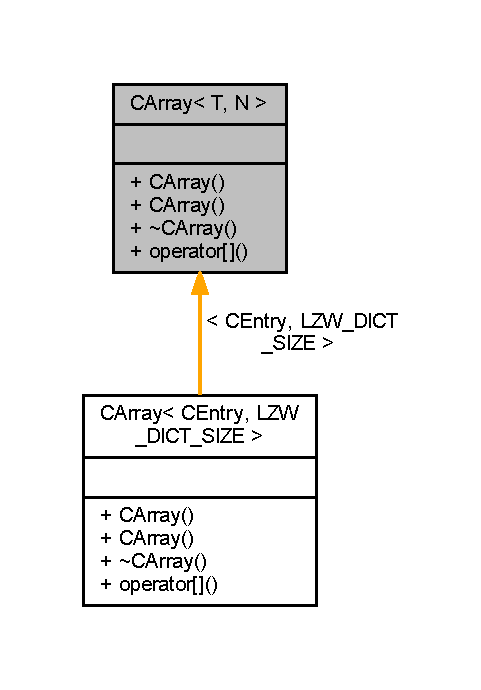
\includegraphics[width=231pt]{class_c_array__inherit__graph}
\end{center}
\end{figure}


Zusammengehörigkeiten von C\+Array$<$ T, N $>$\+:
\nopagebreak
\begin{figure}[H]
\begin{center}
\leavevmode
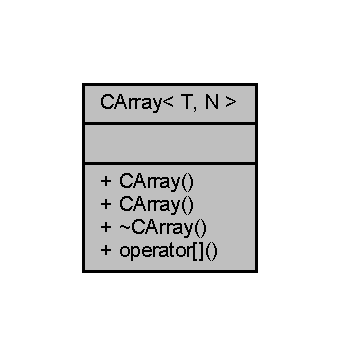
\includegraphics[width=163pt]{class_c_array__coll__graph}
\end{center}
\end{figure}
\subsection*{Öffentliche Methoden}
\begin{DoxyCompactItemize}
\item 
\hyperlink{class_c_array_aa2f1336f8d60cfd1396a920a04a0e0bb}{C\+Array} ()
\begin{DoxyCompactList}\small\item\em Paramenterloser Standartkonstruktor. \end{DoxyCompactList}\item 
\hyperlink{class_c_array_add790ca71782225282e735fabaa36626}{C\+Array} (const \hyperlink{class_c_array}{C\+Array}$<$ T, N $>$ \&copy)
\begin{DoxyCompactList}\small\item\em Kopierkonstruktur Erzeugt eine tiefe Kopie von copy. \end{DoxyCompactList}\item 
virtual \hyperlink{class_c_array_a1aa64db8be620da54c5987f16544a206}{$\sim$\+C\+Array} ()
\begin{DoxyCompactList}\small\item\em Destruktor der Klasse löscht das gesamte Array und macht entries anschließend zum nullptr. \end{DoxyCompactList}\item 
T \& \hyperlink{class_c_array_a81dc8949159e2f4b213d33a5d2b5aec7}{operator\mbox{[}$\,$\mbox{]}} (unsigned int index)
\end{DoxyCompactItemize}


\subsection{Ausführliche Beschreibung}
\subsubsection*{template$<$typename T, unsigned int N$>$\newline
class C\+Array$<$ T, N $>$}

Erzeugt ein Array vom Typ T mit N Elementen Es existiert ein Kopierkonstruktor, der eine tiefe Kopie eines anderen Objekts gleichen Typs erzeugt. Mithilfe des operators \mbox{[}\mbox{]} kann man direkt auf eine Referenz eines Elementes von entries zugreifen. 

\subsection{Beschreibung der Konstruktoren und Destruktoren}
\mbox{\Hypertarget{class_c_array_aa2f1336f8d60cfd1396a920a04a0e0bb}\label{class_c_array_aa2f1336f8d60cfd1396a920a04a0e0bb}} 
\index{C\+Array@{C\+Array}!C\+Array@{C\+Array}}
\index{C\+Array@{C\+Array}!C\+Array@{C\+Array}}
\subsubsection{\texorpdfstring{C\+Array()}{CArray()}\hspace{0.1cm}{\footnotesize\ttfamily [1/2]}}
{\footnotesize\ttfamily template$<$typename T , unsigned int N$>$ \\
\hyperlink{class_c_array}{C\+Array}$<$ T, N $>$\+::\hyperlink{class_c_array}{C\+Array} (\begin{DoxyParamCaption}{ }\end{DoxyParamCaption})}



Paramenterloser Standartkonstruktor. 

\mbox{\Hypertarget{class_c_array_add790ca71782225282e735fabaa36626}\label{class_c_array_add790ca71782225282e735fabaa36626}} 
\index{C\+Array@{C\+Array}!C\+Array@{C\+Array}}
\index{C\+Array@{C\+Array}!C\+Array@{C\+Array}}
\subsubsection{\texorpdfstring{C\+Array()}{CArray()}\hspace{0.1cm}{\footnotesize\ttfamily [2/2]}}
{\footnotesize\ttfamily template$<$typename T, unsigned int N$>$ \\
\hyperlink{class_c_array}{C\+Array}$<$ T, N $>$\+::\hyperlink{class_c_array}{C\+Array} (\begin{DoxyParamCaption}\item[{const \hyperlink{class_c_array}{C\+Array}$<$ T, N $>$ \&}]{copy }\end{DoxyParamCaption})}



Kopierkonstruktur Erzeugt eine tiefe Kopie von copy. 


\begin{DoxyParams}{Parameter}
{\em copy} & Referenz auf zu kopierendes Objekt \\
\hline
\end{DoxyParams}
\mbox{\Hypertarget{class_c_array_a1aa64db8be620da54c5987f16544a206}\label{class_c_array_a1aa64db8be620da54c5987f16544a206}} 
\index{C\+Array@{C\+Array}!````~C\+Array@{$\sim$\+C\+Array}}
\index{````~C\+Array@{$\sim$\+C\+Array}!C\+Array@{C\+Array}}
\subsubsection{\texorpdfstring{$\sim$\+C\+Array()}{~CArray()}}
{\footnotesize\ttfamily template$<$typename T , unsigned int N$>$ \\
\hyperlink{class_c_array}{C\+Array}$<$ T, N $>$\+::$\sim$\hyperlink{class_c_array}{C\+Array} (\begin{DoxyParamCaption}{ }\end{DoxyParamCaption})\hspace{0.3cm}{\ttfamily [virtual]}}



Destruktor der Klasse löscht das gesamte Array und macht entries anschließend zum nullptr. 



\subsection{Dokumentation der Elementfunktionen}
\mbox{\Hypertarget{class_c_array_a81dc8949159e2f4b213d33a5d2b5aec7}\label{class_c_array_a81dc8949159e2f4b213d33a5d2b5aec7}} 
\index{C\+Array@{C\+Array}!operator\mbox{[}\mbox{]}@{operator[]}}
\index{operator\mbox{[}\mbox{]}@{operator[]}!C\+Array@{C\+Array}}
\subsubsection{\texorpdfstring{operator[]()}{operator[]()}}
{\footnotesize\ttfamily template$<$typename T , unsigned int N$>$ \\
T \& \hyperlink{class_c_array}{C\+Array}$<$ T, N $>$\+::operator\mbox{[}$\,$\mbox{]} (\begin{DoxyParamCaption}\item[{unsigned int}]{index }\end{DoxyParamCaption})}

Zugriff auf ein einzelnes Element des Feldes entries 
\begin{DoxyParams}{Parameter}
{\em index} & Stelle des Zugriffs \\
\hline
\end{DoxyParams}
\begin{DoxyReturn}{Rückgabe}
Referenz auf das Element 
\end{DoxyReturn}


Die Dokumentation für diese Klasse wurde erzeugt aufgrund der Datei\+:\begin{DoxyCompactItemize}
\item 
C\+:/portable\+Dev\+Env\+\_\+2017/workspace2017/project/src/\hyperlink{_c_array_8hpp}{C\+Array.\+hpp}\end{DoxyCompactItemize}

\hypertarget{class_c_array_dec}{}\section{C\+Array\+Dec Klassenreferenz}
\label{class_c_array_dec}\index{C\+Array\+Dec@{C\+Array\+Dec}}


L\+ZW Decoder Klasse für die Decodierung erbt von \hyperlink{class_c_dec}{C\+Dec}.  




{\ttfamily \#include $<$C\+Array\+Dec.\+hpp$>$}



Klassendiagramm für C\+Array\+Dec\+:
\nopagebreak
\begin{figure}[H]
\begin{center}
\leavevmode
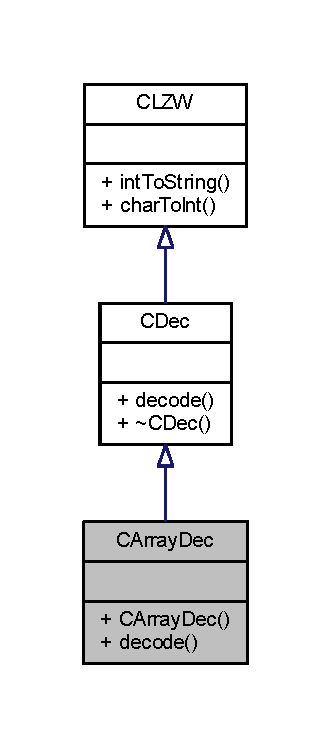
\includegraphics[width=159pt]{class_c_array_dec__inherit__graph}
\end{center}
\end{figure}


Zusammengehörigkeiten von C\+Array\+Dec\+:
\nopagebreak
\begin{figure}[H]
\begin{center}
\leavevmode
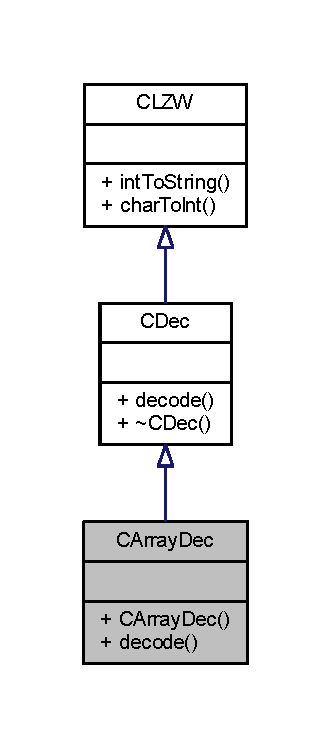
\includegraphics[width=159pt]{class_c_array_dec__coll__graph}
\end{center}
\end{figure}
\subsection*{Öffentliche Methoden}
\begin{DoxyCompactItemize}
\item 
\hyperlink{class_c_array_dec_a23b04c4bfd814351394427a5c867514b}{C\+Array\+Dec} ()
\begin{DoxyCompactList}\small\item\em Parameterloser Konstuktor der Klasse initialisiert das Dicitonary mit den ersten 256 A\+S\+C\+II Zeichen. \end{DoxyCompactList}\item 
std\+::string \hyperlink{class_c_array_dec_a59b83f47506de60b41728d6889d5643a}{decode} (const std\+::vector$<$ unsigned int $>$ \&enc)
\end{DoxyCompactItemize}
\subsection*{Weitere Geerbte Elemente}


\subsection{Ausführliche Beschreibung}
L\+ZW Decoder Klasse für die Decodierung erbt von \hyperlink{class_c_dec}{C\+Dec}. 

\subsection{Beschreibung der Konstruktoren und Destruktoren}
\mbox{\Hypertarget{class_c_array_dec_a23b04c4bfd814351394427a5c867514b}\label{class_c_array_dec_a23b04c4bfd814351394427a5c867514b}} 
\index{C\+Array\+Dec@{C\+Array\+Dec}!C\+Array\+Dec@{C\+Array\+Dec}}
\index{C\+Array\+Dec@{C\+Array\+Dec}!C\+Array\+Dec@{C\+Array\+Dec}}
\subsubsection{\texorpdfstring{C\+Array\+Dec()}{CArrayDec()}}
{\footnotesize\ttfamily C\+Array\+Dec\+::\+C\+Array\+Dec (\begin{DoxyParamCaption}{ }\end{DoxyParamCaption})}



Parameterloser Konstuktor der Klasse initialisiert das Dicitonary mit den ersten 256 A\+S\+C\+II Zeichen. 

Hier ist ein Graph, der zeigt, was diese Funktion aufruft\+:
\nopagebreak
\begin{figure}[H]
\begin{center}
\leavevmode
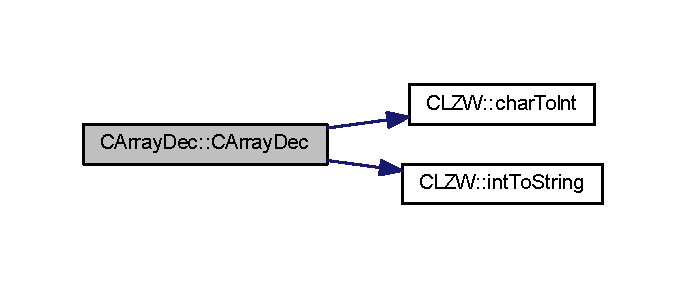
\includegraphics[width=329pt]{class_c_array_dec_a23b04c4bfd814351394427a5c867514b_cgraph}
\end{center}
\end{figure}


\subsection{Dokumentation der Elementfunktionen}
\mbox{\Hypertarget{class_c_array_dec_a59b83f47506de60b41728d6889d5643a}\label{class_c_array_dec_a59b83f47506de60b41728d6889d5643a}} 
\index{C\+Array\+Dec@{C\+Array\+Dec}!decode@{decode}}
\index{decode@{decode}!C\+Array\+Dec@{C\+Array\+Dec}}
\subsubsection{\texorpdfstring{decode()}{decode()}}
{\footnotesize\ttfamily std\+::string C\+Array\+Dec\+::decode (\begin{DoxyParamCaption}\item[{const std\+::vector$<$ unsigned int $>$ \&}]{enc }\end{DoxyParamCaption})}

L\+ZW decoder-\/function 
\begin{DoxyParams}{Parameter}
{\em enc} & decodierender Vector (/ Folge von Indizes ) \\
\hline
\end{DoxyParams}
\begin{DoxyReturn}{Rückgabe}
entschlüsselte Zeichenkette 
\end{DoxyReturn}
Hier ist ein Graph der zeigt, wo diese Funktion aufgerufen wird\+:
\nopagebreak
\begin{figure}[H]
\begin{center}
\leavevmode
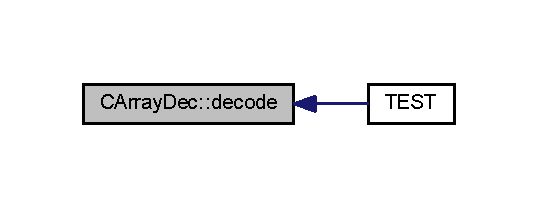
\includegraphics[width=258pt]{class_c_array_dec_a59b83f47506de60b41728d6889d5643a_icgraph}
\end{center}
\end{figure}


Die Dokumentation für diese Klasse wurde erzeugt aufgrund der Dateien\+:\begin{DoxyCompactItemize}
\item 
C\+:/portable\+Dev\+Env\+\_\+2017/workspace2017/project/src/\hyperlink{_c_array_dec_8hpp}{C\+Array\+Dec.\+hpp}\item 
C\+:/portable\+Dev\+Env\+\_\+2017/workspace2017/project/src/\hyperlink{_c_array_dec_8cpp}{C\+Array\+Dec.\+cpp}\end{DoxyCompactItemize}

\hypertarget{class_c_array_enc}{}\section{C\+Array\+Enc Klassenreferenz}
\label{class_c_array_enc}\index{C\+Array\+Enc@{C\+Array\+Enc}}


L\+ZW Encoder Klasse für die Encodierung erbt von \hyperlink{class_c_enc}{C\+Enc}.  




{\ttfamily \#include $<$C\+Array\+Enc.\+hpp$>$}



Klassendiagramm für C\+Array\+Enc\+:
\nopagebreak
\begin{figure}[H]
\begin{center}
\leavevmode
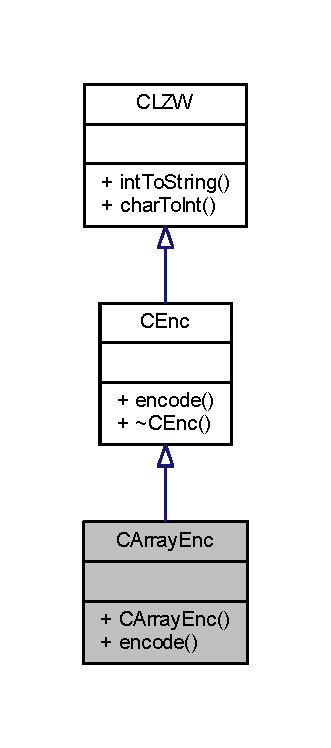
\includegraphics[width=159pt]{class_c_array_enc__inherit__graph}
\end{center}
\end{figure}


Zusammengehörigkeiten von C\+Array\+Enc\+:
\nopagebreak
\begin{figure}[H]
\begin{center}
\leavevmode
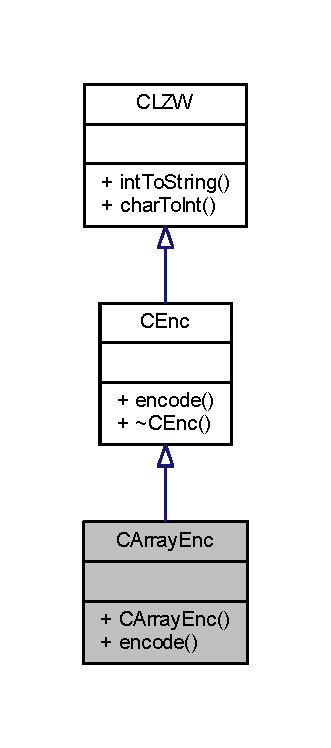
\includegraphics[width=159pt]{class_c_array_enc__coll__graph}
\end{center}
\end{figure}
\subsection*{Öffentliche Methoden}
\begin{DoxyCompactItemize}
\item 
\hyperlink{class_c_array_enc_ad583bca8c7872d055f6118219f657970}{C\+Array\+Enc} ()
\begin{DoxyCompactList}\small\item\em Parameterloser Konstuktor der Klasse initialisiert das Dicitonary mit den ersten 256 A\+S\+C\+II Zeichen. \end{DoxyCompactList}\item 
std\+::vector$<$ unsigned int $>$ \hyperlink{class_c_array_enc_a51984cee678c54c93caf73aa82b596cc}{encode} (const std\+::string \&in)
\end{DoxyCompactItemize}
\subsection*{Weitere Geerbte Elemente}


\subsection{Ausführliche Beschreibung}
L\+ZW Encoder Klasse für die Encodierung erbt von \hyperlink{class_c_enc}{C\+Enc}. 

\subsection{Beschreibung der Konstruktoren und Destruktoren}
\mbox{\Hypertarget{class_c_array_enc_ad583bca8c7872d055f6118219f657970}\label{class_c_array_enc_ad583bca8c7872d055f6118219f657970}} 
\index{C\+Array\+Enc@{C\+Array\+Enc}!C\+Array\+Enc@{C\+Array\+Enc}}
\index{C\+Array\+Enc@{C\+Array\+Enc}!C\+Array\+Enc@{C\+Array\+Enc}}
\subsubsection{\texorpdfstring{C\+Array\+Enc()}{CArrayEnc()}}
{\footnotesize\ttfamily C\+Array\+Enc\+::\+C\+Array\+Enc (\begin{DoxyParamCaption}{ }\end{DoxyParamCaption})}



Parameterloser Konstuktor der Klasse initialisiert das Dicitonary mit den ersten 256 A\+S\+C\+II Zeichen. 

Hier ist ein Graph, der zeigt, was diese Funktion aufruft\+:
\nopagebreak
\begin{figure}[H]
\begin{center}
\leavevmode
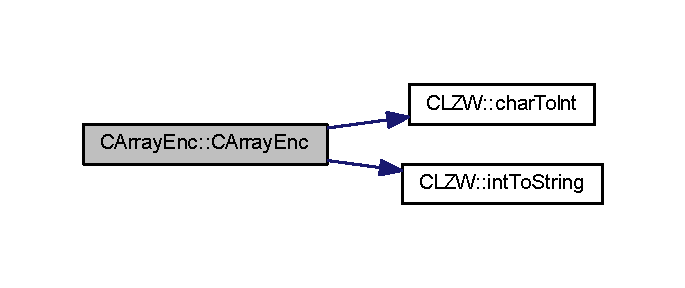
\includegraphics[width=329pt]{class_c_array_enc_ad583bca8c7872d055f6118219f657970_cgraph}
\end{center}
\end{figure}


\subsection{Dokumentation der Elementfunktionen}
\mbox{\Hypertarget{class_c_array_enc_a51984cee678c54c93caf73aa82b596cc}\label{class_c_array_enc_a51984cee678c54c93caf73aa82b596cc}} 
\index{C\+Array\+Enc@{C\+Array\+Enc}!encode@{encode}}
\index{encode@{encode}!C\+Array\+Enc@{C\+Array\+Enc}}
\subsubsection{\texorpdfstring{encode()}{encode()}}
{\footnotesize\ttfamily std\+::vector$<$ unsigned int $>$ C\+Array\+Enc\+::encode (\begin{DoxyParamCaption}\item[{const std\+::string \&}]{in }\end{DoxyParamCaption})}

L\+ZW encoder-\/function 
\begin{DoxyParams}{Parameter}
{\em in} & zu komprimierende Zeichenkette \\
\hline
\end{DoxyParams}
\begin{DoxyReturn}{Rückgabe}
kompimierte Zeichenkette als vector 
\end{DoxyReturn}
Hier ist ein Graph der zeigt, wo diese Funktion aufgerufen wird\+:
\nopagebreak
\begin{figure}[H]
\begin{center}
\leavevmode
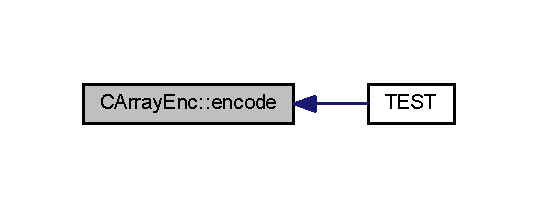
\includegraphics[width=258pt]{class_c_array_enc_a51984cee678c54c93caf73aa82b596cc_icgraph}
\end{center}
\end{figure}


Die Dokumentation für diese Klasse wurde erzeugt aufgrund der Dateien\+:\begin{DoxyCompactItemize}
\item 
C\+:/portable\+Dev\+Env\+\_\+2017/workspace2017/project/src/\hyperlink{_c_array_enc_8hpp}{C\+Array\+Enc.\+hpp}\item 
C\+:/portable\+Dev\+Env\+\_\+2017/workspace2017/project/src/\hyperlink{_c_array_enc_8cpp}{C\+Array\+Enc.\+cpp}\end{DoxyCompactItemize}

\hypertarget{class_c_counter}{}\section{C\+Counter Klassenreferenz}
\label{class_c_counter}\index{C\+Counter@{C\+Counter}}


Klasse \hyperlink{class_c_counter}{C\+Counter} zum Setzen, Inkrementieren und Vergleichen von Zählerständen.  




{\ttfamily \#include $<$C\+Counter.\+hpp$>$}



Klassendiagramm für C\+Counter\+:
\nopagebreak
\begin{figure}[H]
\begin{center}
\leavevmode
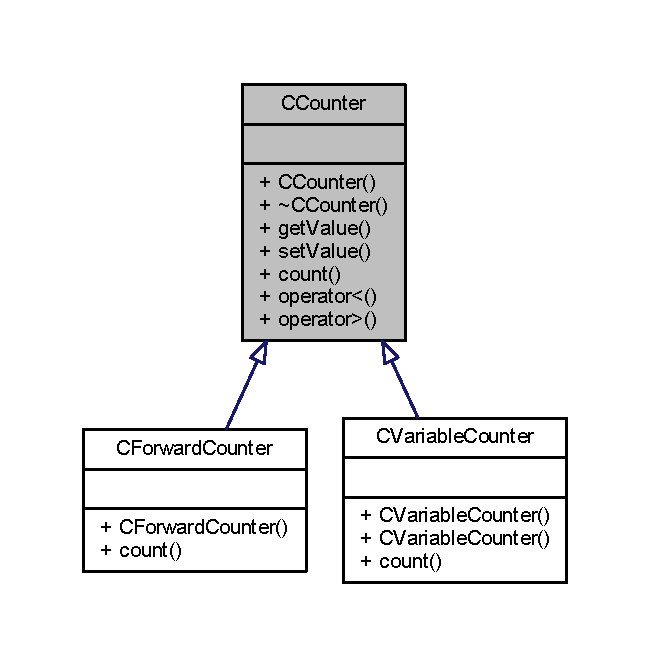
\includegraphics[width=312pt]{class_c_counter__inherit__graph}
\end{center}
\end{figure}


Zusammengehörigkeiten von C\+Counter\+:
\nopagebreak
\begin{figure}[H]
\begin{center}
\leavevmode
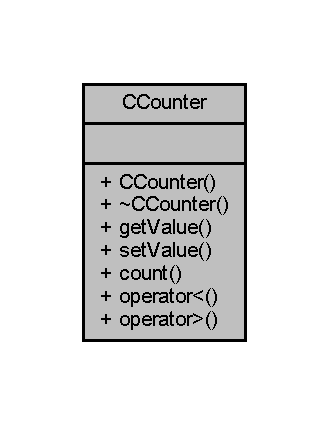
\includegraphics[width=158pt]{class_c_counter__coll__graph}
\end{center}
\end{figure}
\subsection*{Öffentliche Methoden}
\begin{DoxyCompactItemize}
\item 
\hyperlink{class_c_counter_ab83c6f9600beb5686747493da731a04c}{C\+Counter} ()
\item 
virtual \hyperlink{class_c_counter_a1af3cc000781fcd67b9e4fe1b25fbc9c}{$\sim$\+C\+Counter} ()
\item 
int \hyperlink{class_c_counter_ad91db4cd517159f7cbb7d3976eede482}{get\+Value} () const
\item 
void \hyperlink{class_c_counter_ac41245afdd95c0149e99bad21696a372}{set\+Value} (int value)
\item 
virtual void \hyperlink{class_c_counter_a90f3e164f3fc1dcf91044702d6940c4d}{count} ()
\item 
bool \hyperlink{class_c_counter_ac43e4c4cb447d22636ac208d426d95eb}{operator$<$} (const \hyperlink{class_c_counter}{C\+Counter} \&other) const
\item 
bool \hyperlink{class_c_counter_a23decf75e74ddfd25feb11ae6aad9c8a}{operator$>$} (const \hyperlink{class_c_counter}{C\+Counter} \&other) const
\end{DoxyCompactItemize}


\subsection{Ausführliche Beschreibung}
Klasse \hyperlink{class_c_counter}{C\+Counter} zum Setzen, Inkrementieren und Vergleichen von Zählerständen. 

\hyperlink{class_c_counter_ab83c6f9600beb5686747493da731a04c}{C\+Counter()} ist der parameterlose Konstruktor \hyperlink{class_c_counter_a1af3cc000781fcd67b9e4fe1b25fbc9c}{$\sim$\+C\+Counter()} ist der Destruktor int \hyperlink{class_c_counter_ad91db4cd517159f7cbb7d3976eede482}{get\+Value()} liefert den Zählerstand void \hyperlink{class_c_counter_ac41245afdd95c0149e99bad21696a372}{set\+Value(int)} setzt den Zählerstand void \hyperlink{class_c_counter_a90f3e164f3fc1dcf91044702d6940c4d}{count()} inkrementiert den Zählerstand bool operator$<$(\+C\+Counter\&) prüft, ob Argument größeren Zählerstand besitzt bool operator$>$(\+C\+Counter\&)

int m\+\_\+value ist die private Membervariable für den Zählerstand. Wir verwenden die Konvention, dass der Namen privater Membervariablen mit m\+\_\+ beginnt. 

\subsection{Beschreibung der Konstruktoren und Destruktoren}
\mbox{\Hypertarget{class_c_counter_ab83c6f9600beb5686747493da731a04c}\label{class_c_counter_ab83c6f9600beb5686747493da731a04c}} 
\index{C\+Counter@{C\+Counter}!C\+Counter@{C\+Counter}}
\index{C\+Counter@{C\+Counter}!C\+Counter@{C\+Counter}}
\subsubsection{\texorpdfstring{C\+Counter()}{CCounter()}}
{\footnotesize\ttfamily C\+Counter\+::\+C\+Counter (\begin{DoxyParamCaption}{ }\end{DoxyParamCaption})}

Deklaration des parameterlosen Konstruktors. \mbox{\Hypertarget{class_c_counter_a1af3cc000781fcd67b9e4fe1b25fbc9c}\label{class_c_counter_a1af3cc000781fcd67b9e4fe1b25fbc9c}} 
\index{C\+Counter@{C\+Counter}!````~C\+Counter@{$\sim$\+C\+Counter}}
\index{````~C\+Counter@{$\sim$\+C\+Counter}!C\+Counter@{C\+Counter}}
\subsubsection{\texorpdfstring{$\sim$\+C\+Counter()}{~CCounter()}}
{\footnotesize\ttfamily C\+Counter\+::$\sim$\+C\+Counter (\begin{DoxyParamCaption}{ }\end{DoxyParamCaption})\hspace{0.3cm}{\ttfamily [virtual]}}

Destruktor von \hyperlink{class_c_counter}{C\+Counter} 

\subsection{Dokumentation der Elementfunktionen}
\mbox{\Hypertarget{class_c_counter_a90f3e164f3fc1dcf91044702d6940c4d}\label{class_c_counter_a90f3e164f3fc1dcf91044702d6940c4d}} 
\index{C\+Counter@{C\+Counter}!count@{count}}
\index{count@{count}!C\+Counter@{C\+Counter}}
\subsubsection{\texorpdfstring{count()}{count()}}
{\footnotesize\ttfamily void C\+Counter\+::count (\begin{DoxyParamCaption}{ }\end{DoxyParamCaption})\hspace{0.3cm}{\ttfamily [virtual]}}

Inkrementiert den Zählerstand um 1 

Erneute Implementation in \hyperlink{class_c_variable_counter_a693c27202acd18d53c4642ce642927bc}{C\+Variable\+Counter} und \hyperlink{class_c_forward_counter_afc451afa9f8b76f70b28c08982265a86}{C\+Forward\+Counter}.

Hier ist ein Graph der zeigt, wo diese Funktion aufgerufen wird\+:
\nopagebreak
\begin{figure}[H]
\begin{center}
\leavevmode
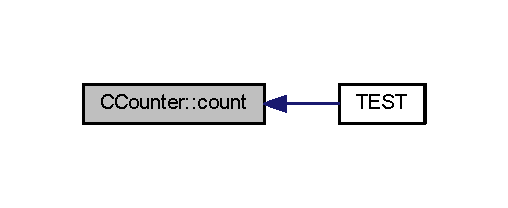
\includegraphics[width=244pt]{class_c_counter_a90f3e164f3fc1dcf91044702d6940c4d_icgraph}
\end{center}
\end{figure}
\mbox{\Hypertarget{class_c_counter_ad91db4cd517159f7cbb7d3976eede482}\label{class_c_counter_ad91db4cd517159f7cbb7d3976eede482}} 
\index{C\+Counter@{C\+Counter}!get\+Value@{get\+Value}}
\index{get\+Value@{get\+Value}!C\+Counter@{C\+Counter}}
\subsubsection{\texorpdfstring{get\+Value()}{getValue()}}
{\footnotesize\ttfamily int C\+Counter\+::get\+Value (\begin{DoxyParamCaption}{ }\end{DoxyParamCaption}) const}

Gib den Wert der Zählervariable aus. \begin{DoxyReturn}{Rückgabe}
enthält den Wert der Zählervariable m\+\_\+value. 
\end{DoxyReturn}
Hier ist ein Graph der zeigt, wo diese Funktion aufgerufen wird\+:
\nopagebreak
\begin{figure}[H]
\begin{center}
\leavevmode
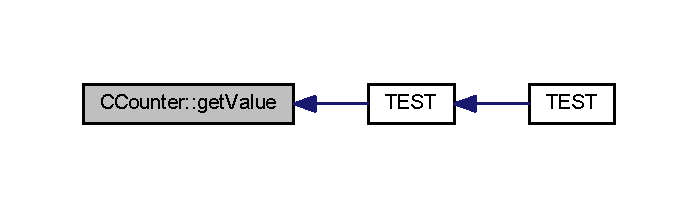
\includegraphics[width=335pt]{class_c_counter_ad91db4cd517159f7cbb7d3976eede482_icgraph}
\end{center}
\end{figure}
\mbox{\Hypertarget{class_c_counter_ac43e4c4cb447d22636ac208d426d95eb}\label{class_c_counter_ac43e4c4cb447d22636ac208d426d95eb}} 
\index{C\+Counter@{C\+Counter}!operator$<$@{operator$<$}}
\index{operator$<$@{operator$<$}!C\+Counter@{C\+Counter}}
\subsubsection{\texorpdfstring{operator$<$()}{operator<()}}
{\footnotesize\ttfamily bool C\+Counter\+::operator$<$ (\begin{DoxyParamCaption}\item[{const \hyperlink{class_c_counter}{C\+Counter} \&}]{other }\end{DoxyParamCaption}) const}

Prüft, ob der Zählerstand kleiner ist, als der Eingabeparameter. Die Memberfunktion \hyperlink{class_c_counter_ac43e4c4cb447d22636ac208d426d95eb}{operator$<$()} steht für den Operator $<$ . 
\begin{DoxyParams}{Parameter}
{\em other} & ist der Eingabeparameter. \\
\hline
\end{DoxyParams}
\begin{DoxyReturn}{Rückgabe}
ist wahr, falls der Zählerstand kleiner als der Eingabeparameter ist. 
\end{DoxyReturn}
\mbox{\Hypertarget{class_c_counter_a23decf75e74ddfd25feb11ae6aad9c8a}\label{class_c_counter_a23decf75e74ddfd25feb11ae6aad9c8a}} 
\index{C\+Counter@{C\+Counter}!operator$>$@{operator$>$}}
\index{operator$>$@{operator$>$}!C\+Counter@{C\+Counter}}
\subsubsection{\texorpdfstring{operator$>$()}{operator>()}}
{\footnotesize\ttfamily bool C\+Counter\+::operator$>$ (\begin{DoxyParamCaption}\item[{const \hyperlink{class_c_counter}{C\+Counter} \&}]{other }\end{DoxyParamCaption}) const}

Prüft, ob der Zählerstand größer ist, als der Eingabeparameter. Die Memberfunktion \hyperlink{class_c_counter_a23decf75e74ddfd25feb11ae6aad9c8a}{operator$>$()} steht für den Operator $>$ . 
\begin{DoxyParams}{Parameter}
{\em other} & ist der Eingabeparameter. \\
\hline
\end{DoxyParams}
\begin{DoxyReturn}{Rückgabe}
ist wahr, falls der Zählerstand größer als der Eingabeparameter ist. 
\end{DoxyReturn}
\mbox{\Hypertarget{class_c_counter_ac41245afdd95c0149e99bad21696a372}\label{class_c_counter_ac41245afdd95c0149e99bad21696a372}} 
\index{C\+Counter@{C\+Counter}!set\+Value@{set\+Value}}
\index{set\+Value@{set\+Value}!C\+Counter@{C\+Counter}}
\subsubsection{\texorpdfstring{set\+Value()}{setValue()}}
{\footnotesize\ttfamily void C\+Counter\+::set\+Value (\begin{DoxyParamCaption}\item[{int}]{value }\end{DoxyParamCaption})}

Setze die Zählervariable. 
\begin{DoxyParams}{Parameter}
{\em value} & Die Zählervariable m\+\_\+value wird auf den Wert der Parametervariable value gesetzt. \\
\hline
\end{DoxyParams}
Hier ist ein Graph der zeigt, wo diese Funktion aufgerufen wird\+:
\nopagebreak
\begin{figure}[H]
\begin{center}
\leavevmode
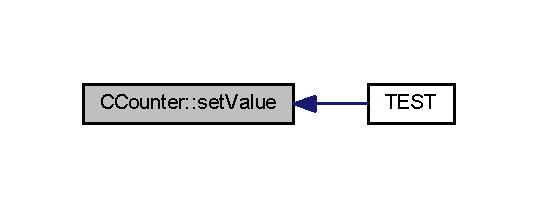
\includegraphics[width=258pt]{class_c_counter_ac41245afdd95c0149e99bad21696a372_icgraph}
\end{center}
\end{figure}


Die Dokumentation für diese Klasse wurde erzeugt aufgrund der Dateien\+:\begin{DoxyCompactItemize}
\item 
C\+:/portable\+Dev\+Env\+\_\+2017/workspace2017/\+Blatt2/src/\hyperlink{_c_counter_8hpp}{C\+Counter.\+hpp}\item 
C\+:/portable\+Dev\+Env\+\_\+2017/workspace2017/\+Blatt2/src/\hyperlink{_c_counter_8cpp}{C\+Counter.\+cpp}\end{DoxyCompactItemize}

\hypertarget{class_c_dec}{}\section{C\+Dec Klassenreferenz}
\label{class_c_dec}\index{C\+Dec@{C\+Dec}}


Abstrakte Basisklasse für die Decoder.  




{\ttfamily \#include $<$C\+Dec.\+hpp$>$}



Klassendiagramm für C\+Dec\+:
\nopagebreak
\begin{figure}[H]
\begin{center}
\leavevmode
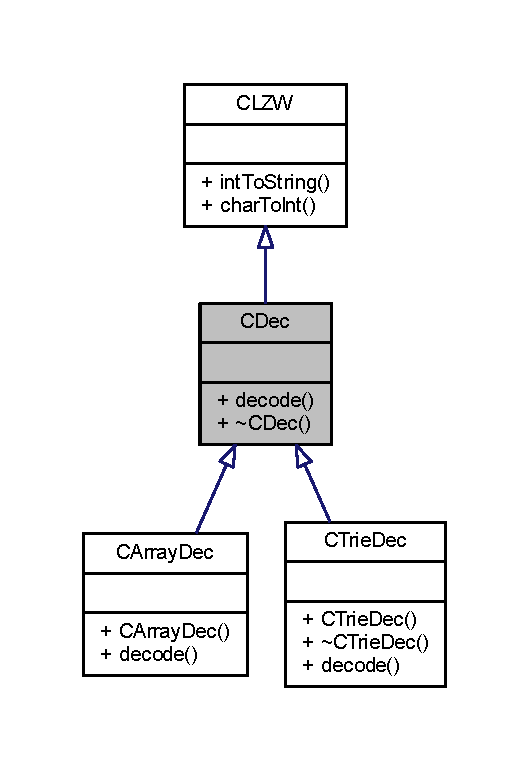
\includegraphics[width=254pt]{class_c_dec__inherit__graph}
\end{center}
\end{figure}


Zusammengehörigkeiten von C\+Dec\+:
\nopagebreak
\begin{figure}[H]
\begin{center}
\leavevmode
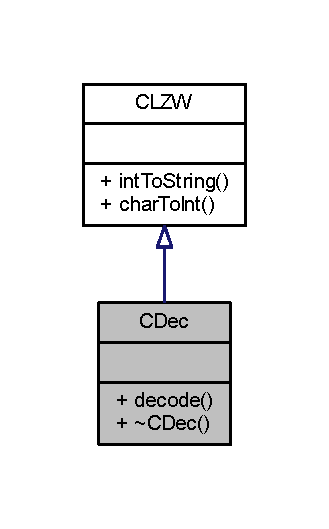
\includegraphics[width=158pt]{class_c_dec__coll__graph}
\end{center}
\end{figure}
\subsection*{Öffentliche Methoden}
\begin{DoxyCompactItemize}
\item 
virtual string \hyperlink{class_c_dec_a88c60d9d4285714347a3bae0ef0a319d}{decode} (const vector$<$ unsigned int $>$ \&in)=0
\item 
virtual \hyperlink{class_c_dec_a66bbd291c322a9ca78c80284eb9c5acf}{$\sim$\+C\+Dec} ()
\begin{DoxyCompactList}\small\item\em Virtueller Destruktor. \end{DoxyCompactList}\end{DoxyCompactItemize}
\subsection*{Weitere Geerbte Elemente}


\subsection{Ausführliche Beschreibung}
Abstrakte Basisklasse für die Decoder. 

Abstrakte Basisklasse für die Decoder. \hyperlink{class_c_dec}{C\+Dec} erbt von \hyperlink{class_c_l_z_w}{C\+L\+ZW}. Basisklasse der Encoderklassen \hyperlink{class_c_array_dec}{C\+Array\+Dec} und \hyperlink{class_c_trie_dec}{C\+Trie\+Dec}. Von dieser Klasse \hyperlink{class_c_dec}{C\+Dec} selbst können keine Instanzen erstellt werden, sie ist abstrakt. 

\subsection{Beschreibung der Konstruktoren und Destruktoren}
\mbox{\Hypertarget{class_c_dec_a66bbd291c322a9ca78c80284eb9c5acf}\label{class_c_dec_a66bbd291c322a9ca78c80284eb9c5acf}} 
\index{C\+Dec@{C\+Dec}!````~C\+Dec@{$\sim$\+C\+Dec}}
\index{````~C\+Dec@{$\sim$\+C\+Dec}!C\+Dec@{C\+Dec}}
\subsubsection{\texorpdfstring{$\sim$\+C\+Dec()}{~CDec()}}
{\footnotesize\ttfamily C\+Dec\+::$\sim$\+C\+Dec (\begin{DoxyParamCaption}{ }\end{DoxyParamCaption})\hspace{0.3cm}{\ttfamily [virtual]}}



Virtueller Destruktor. 



\subsection{Dokumentation der Elementfunktionen}
\mbox{\Hypertarget{class_c_dec_a88c60d9d4285714347a3bae0ef0a319d}\label{class_c_dec_a88c60d9d4285714347a3bae0ef0a319d}} 
\index{C\+Dec@{C\+Dec}!decode@{decode}}
\index{decode@{decode}!C\+Dec@{C\+Dec}}
\subsubsection{\texorpdfstring{decode()}{decode()}}
{\footnotesize\ttfamily virtual string C\+Dec\+::decode (\begin{DoxyParamCaption}\item[{const vector$<$ unsigned int $>$ \&}]{in }\end{DoxyParamCaption})\hspace{0.3cm}{\ttfamily [pure virtual]}}

decodiert (restauriert) den String in mit Hilfe des L\+Z\+W-\/\+Algorithmus 
\begin{DoxyParams}{Parameter}
{\em in} & Vektor der zu decodierenden Indexwerte \\
\hline
\end{DoxyParams}
\begin{DoxyReturn}{Rückgabe}
decodierter Zählerstand 
\end{DoxyReturn}


Die Dokumentation für diese Klasse wurde erzeugt aufgrund der Dateien\+:\begin{DoxyCompactItemize}
\item 
C\+:/portable\+Dev\+Env\+\_\+2017/workspace2017/project/src/\hyperlink{_c_dec_8hpp}{C\+Dec.\+hpp}\item 
C\+:/portable\+Dev\+Env\+\_\+2017/workspace2017/project/src/\hyperlink{_c_dec_8cpp}{C\+Dec.\+cpp}\end{DoxyCompactItemize}

\hypertarget{class_c_double_hashing}{}\section{C\+Double\+Hashing Klassenreferenz}
\label{class_c_double_hashing}\index{C\+Double\+Hashing@{C\+Double\+Hashing}}


{\ttfamily \#include $<$C\+Double\+Hashing.\+hpp$>$}



Zusammengehörigkeiten von C\+Double\+Hashing\+:
\nopagebreak
\begin{figure}[H]
\begin{center}
\leavevmode
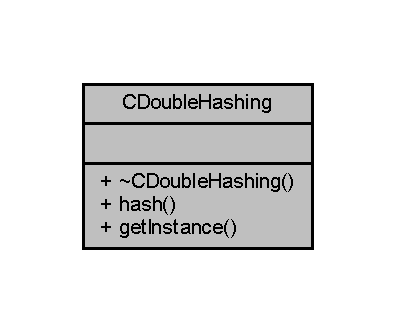
\includegraphics[width=190pt]{class_c_double_hashing__coll__graph}
\end{center}
\end{figure}
\subsection*{Öffentliche Methoden}
\begin{DoxyCompactItemize}
\item 
virtual \hyperlink{class_c_double_hashing_a4ffc5039f507c1def31ca5bc672ce8e2}{$\sim$\+C\+Double\+Hashing} ()
\begin{DoxyCompactList}\small\item\em Standard Destruktor. \end{DoxyCompactList}\item 
unsigned int \hyperlink{class_c_double_hashing_a0ec6ff1eb94927284b8e6fe4f650ecf9}{hash} (unsigned int I, unsigned int J, unsigned int dict\+\_\+size, unsigned int attempt)
\end{DoxyCompactItemize}
\subsection*{Öffentliche, statische Methoden}
\begin{DoxyCompactItemize}
\item 
static \hyperlink{class_c_double_hashing}{C\+Double\+Hashing} \& \hyperlink{class_c_double_hashing_a3917e940f9bac5c981156062eb2b1169}{get\+Instance} ()
\end{DoxyCompactItemize}


\subsection{Beschreibung der Konstruktoren und Destruktoren}
\mbox{\Hypertarget{class_c_double_hashing_a4ffc5039f507c1def31ca5bc672ce8e2}\label{class_c_double_hashing_a4ffc5039f507c1def31ca5bc672ce8e2}} 
\index{C\+Double\+Hashing@{C\+Double\+Hashing}!````~C\+Double\+Hashing@{$\sim$\+C\+Double\+Hashing}}
\index{````~C\+Double\+Hashing@{$\sim$\+C\+Double\+Hashing}!C\+Double\+Hashing@{C\+Double\+Hashing}}
\subsubsection{\texorpdfstring{$\sim$\+C\+Double\+Hashing()}{~CDoubleHashing()}}
{\footnotesize\ttfamily C\+Double\+Hashing\+::$\sim$\+C\+Double\+Hashing (\begin{DoxyParamCaption}{ }\end{DoxyParamCaption})\hspace{0.3cm}{\ttfamily [virtual]}}



Standard Destruktor. 



\subsection{Dokumentation der Elementfunktionen}
\mbox{\Hypertarget{class_c_double_hashing_a3917e940f9bac5c981156062eb2b1169}\label{class_c_double_hashing_a3917e940f9bac5c981156062eb2b1169}} 
\index{C\+Double\+Hashing@{C\+Double\+Hashing}!get\+Instance@{get\+Instance}}
\index{get\+Instance@{get\+Instance}!C\+Double\+Hashing@{C\+Double\+Hashing}}
\subsubsection{\texorpdfstring{get\+Instance()}{getInstance()}}
{\footnotesize\ttfamily \hyperlink{class_c_double_hashing}{C\+Double\+Hashing} \& C\+Double\+Hashing\+::get\+Instance (\begin{DoxyParamCaption}{ }\end{DoxyParamCaption})\hspace{0.3cm}{\ttfamily [static]}}

Einzige Möglichkeit an ein Objekt dieser Klasse zu gelangen static -\/$>$ Singleton, nur Objekt der Klasse vorhanden \begin{DoxyReturn}{Rückgabe}
Objekt der Klasse 
\end{DoxyReturn}
Hier ist ein Graph der zeigt, wo diese Funktion aufgerufen wird\+:
\nopagebreak
\begin{figure}[H]
\begin{center}
\leavevmode
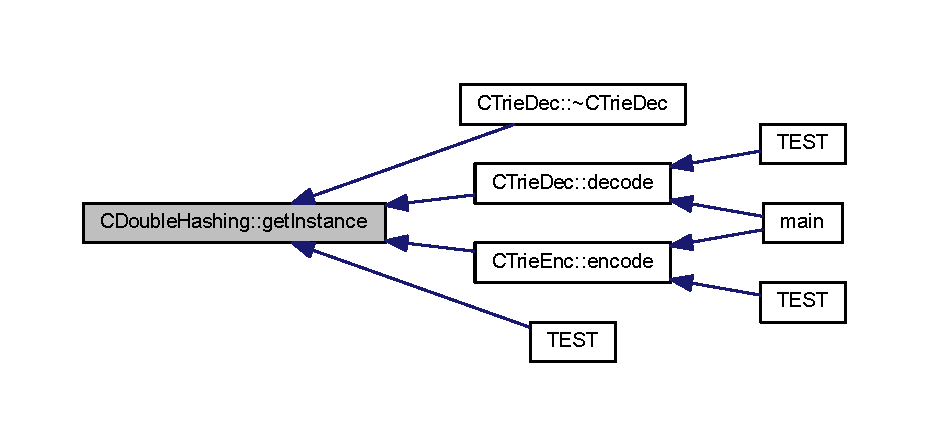
\includegraphics[width=350pt]{class_c_double_hashing_a3917e940f9bac5c981156062eb2b1169_icgraph}
\end{center}
\end{figure}
\mbox{\Hypertarget{class_c_double_hashing_a0ec6ff1eb94927284b8e6fe4f650ecf9}\label{class_c_double_hashing_a0ec6ff1eb94927284b8e6fe4f650ecf9}} 
\index{C\+Double\+Hashing@{C\+Double\+Hashing}!hash@{hash}}
\index{hash@{hash}!C\+Double\+Hashing@{C\+Double\+Hashing}}
\subsubsection{\texorpdfstring{hash()}{hash()}}
{\footnotesize\ttfamily unsigned int C\+Double\+Hashing\+::hash (\begin{DoxyParamCaption}\item[{unsigned int}]{I,  }\item[{unsigned int}]{J,  }\item[{unsigned int}]{dict\+\_\+size,  }\item[{unsigned int}]{attempt }\end{DoxyParamCaption})}

individuelle Hashing Funktion, doppeltes Hashing 
\begin{DoxyParams}{Parameter}
{\em I} & Elternposition \\
\hline
{\em J} & A\+S\+C\+II Wert des neu eingelesenen Zeichens \\
\hline
{\em dict\+\_\+size} & Größe des Dictionarys \\
\hline
{\em attempt} & Anzahl der Hashversuches \\
\hline
\end{DoxyParams}
\begin{DoxyReturn}{Rückgabe}
Hashwert 
\end{DoxyReturn}
Hier ist ein Graph der zeigt, wo diese Funktion aufgerufen wird\+:
\nopagebreak
\begin{figure}[H]
\begin{center}
\leavevmode
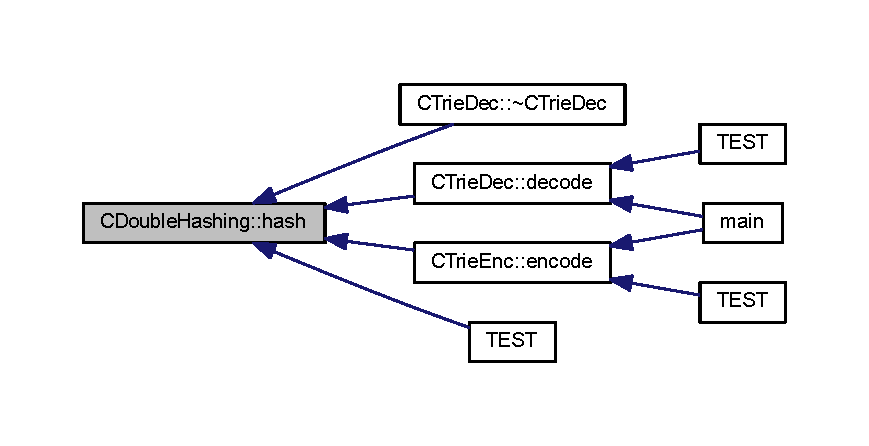
\includegraphics[width=350pt]{class_c_double_hashing_a0ec6ff1eb94927284b8e6fe4f650ecf9_icgraph}
\end{center}
\end{figure}


Die Dokumentation für diese Klasse wurde erzeugt aufgrund der Dateien\+:\begin{DoxyCompactItemize}
\item 
C\+:/portable\+Dev\+Env\+\_\+2017/workspace2017/project/src/\hyperlink{_c_double_hashing_8hpp}{C\+Double\+Hashing.\+hpp}\item 
C\+:/portable\+Dev\+Env\+\_\+2017/workspace2017/project/src/\hyperlink{_c_double_hashing_8cpp}{C\+Double\+Hashing.\+cpp}\end{DoxyCompactItemize}

\hypertarget{class_c_enc}{}\section{C\+Enc Klassenreferenz}
\label{class_c_enc}\index{C\+Enc@{C\+Enc}}


Abstrakte Basisklasse für die Encoder.  




{\ttfamily \#include $<$C\+Enc.\+hpp$>$}



Klassendiagramm für C\+Enc\+:
\nopagebreak
\begin{figure}[H]
\begin{center}
\leavevmode
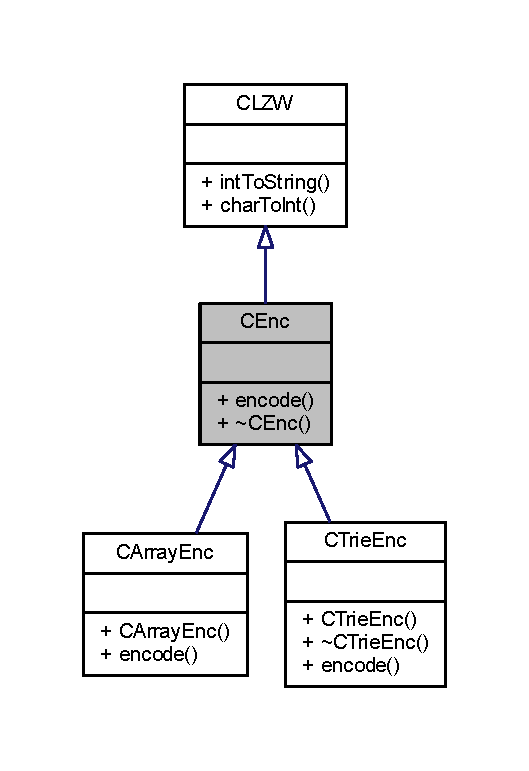
\includegraphics[width=254pt]{class_c_enc__inherit__graph}
\end{center}
\end{figure}


Zusammengehörigkeiten von C\+Enc\+:
\nopagebreak
\begin{figure}[H]
\begin{center}
\leavevmode
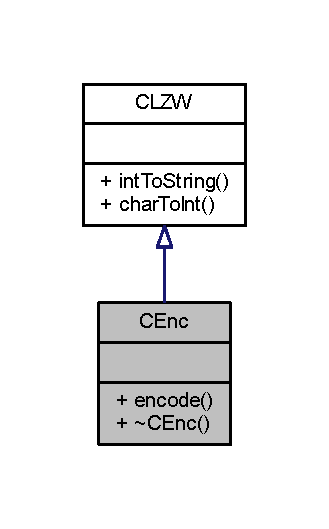
\includegraphics[width=158pt]{class_c_enc__coll__graph}
\end{center}
\end{figure}
\subsection*{Öffentliche Methoden}
\begin{DoxyCompactItemize}
\item 
virtual vector$<$ unsigned int $>$ \hyperlink{class_c_enc_a745a77d134a9abaaf788d47b7a235229}{encode} (const string \&in)=0
\item 
virtual \hyperlink{class_c_enc_a95603c8fc5edf44032b8f7aad8be6517}{$\sim$\+C\+Enc} ()
\end{DoxyCompactItemize}
\subsection*{Weitere Geerbte Elemente}


\subsection{Ausführliche Beschreibung}
Abstrakte Basisklasse für die Encoder. 

Abstrakte Basisklasse für die Encodierung. \hyperlink{class_c_enc}{C\+Enc} erbt von \hyperlink{class_c_l_z_w}{C\+L\+ZW}. Basisklasse der Encoderklassen \hyperlink{class_c_array_enc}{C\+Array\+Enc} und \hyperlink{class_c_trie_enc}{C\+Trie\+Enc}. Von dieser Klasse \hyperlink{class_c_enc}{C\+Enc} selbst können keine Instanzen erstellt werden, sie ist abstrakt. 

\subsection{Beschreibung der Konstruktoren und Destruktoren}
\mbox{\Hypertarget{class_c_enc_a95603c8fc5edf44032b8f7aad8be6517}\label{class_c_enc_a95603c8fc5edf44032b8f7aad8be6517}} 
\index{C\+Enc@{C\+Enc}!````~C\+Enc@{$\sim$\+C\+Enc}}
\index{````~C\+Enc@{$\sim$\+C\+Enc}!C\+Enc@{C\+Enc}}
\subsubsection{\texorpdfstring{$\sim$\+C\+Enc()}{~CEnc()}}
{\footnotesize\ttfamily C\+Enc\+::$\sim$\+C\+Enc (\begin{DoxyParamCaption}{ }\end{DoxyParamCaption})\hspace{0.3cm}{\ttfamily [virtual]}}



\subsection{Dokumentation der Elementfunktionen}
\mbox{\Hypertarget{class_c_enc_a745a77d134a9abaaf788d47b7a235229}\label{class_c_enc_a745a77d134a9abaaf788d47b7a235229}} 
\index{C\+Enc@{C\+Enc}!encode@{encode}}
\index{encode@{encode}!C\+Enc@{C\+Enc}}
\subsubsection{\texorpdfstring{encode()}{encode()}}
{\footnotesize\ttfamily virtual vector$<$unsigned int$>$ C\+Enc\+::encode (\begin{DoxyParamCaption}\item[{const string \&}]{in }\end{DoxyParamCaption})\hspace{0.3cm}{\ttfamily [pure virtual]}}

encodiert (komprimiert) den String in mit Hilfe des L\+Z\+W-\/\+Algorithmus 
\begin{DoxyParams}{Parameter}
{\em in} & String der zu encodierenden Zeichenfolge \\
\hline
\end{DoxyParams}
\begin{DoxyReturn}{Rückgabe}
Vektor der zu übertragenden Indexwerte 
\end{DoxyReturn}


Die Dokumentation für diese Klasse wurde erzeugt aufgrund der Dateien\+:\begin{DoxyCompactItemize}
\item 
C\+:/portable\+Dev\+Env\+\_\+2017/workspace2017/project/src/\hyperlink{_c_enc_8hpp}{C\+Enc.\+hpp}\item 
C\+:/portable\+Dev\+Env\+\_\+2017/workspace2017/project/src/\hyperlink{_c_enc_8cpp}{C\+Enc.\+cpp}\end{DoxyCompactItemize}

\hypertarget{class_c_entry}{}\section{C\+Entry Klassenreferenz}
\label{class_c_entry}\index{C\+Entry@{C\+Entry}}


Enthält Zeichenketten und Anzahl der Objekte dieser Klasse Wird später von \hyperlink{class_c_knot}{C\+Knot} benötigt/erweitert.  




{\ttfamily \#include $<$C\+Entry.\+hpp$>$}



Klassendiagramm für C\+Entry\+:
\nopagebreak
\begin{figure}[H]
\begin{center}
\leavevmode
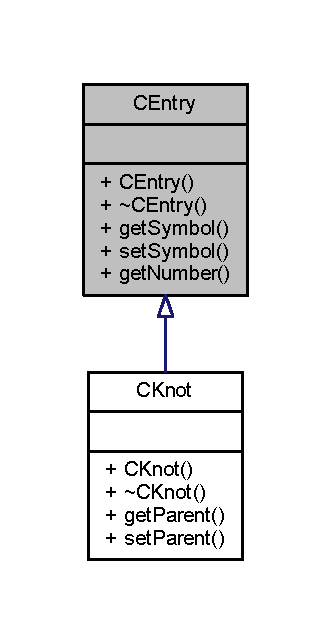
\includegraphics[width=159pt]{class_c_entry__inherit__graph}
\end{center}
\end{figure}


Zusammengehörigkeiten von C\+Entry\+:
\nopagebreak
\begin{figure}[H]
\begin{center}
\leavevmode
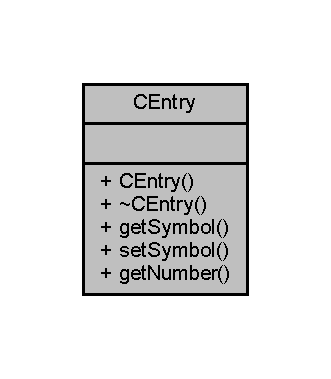
\includegraphics[width=159pt]{class_c_entry__coll__graph}
\end{center}
\end{figure}
\subsection*{Öffentliche Methoden}
\begin{DoxyCompactItemize}
\item 
\hyperlink{class_c_entry_a4faded7dce7c143eeb3c96de4071848d}{C\+Entry} ()
\item 
virtual \hyperlink{class_c_entry_adb596f3be932c1db3d6072a9d6d26f5e}{$\sim$\+C\+Entry} ()
\item 
const std\+::string \& \hyperlink{class_c_entry_aede4d6e03efa3abb0ed56349edb5b86d}{get\+Symbol} () const
\item 
void \hyperlink{class_c_entry_a2ac2cbee24817ff5b67e09f03a952e77}{set\+Symbol} (std\+::string symbol)
\end{DoxyCompactItemize}
\subsection*{Öffentliche, statische Methoden}
\begin{DoxyCompactItemize}
\item 
static unsigned int \hyperlink{class_c_entry_a6e8cde8d4a78cc65fceeb5f0430a2b55}{get\+Number} ()
\end{DoxyCompactItemize}


\subsection{Ausführliche Beschreibung}
Enthält Zeichenketten und Anzahl der Objekte dieser Klasse Wird später von \hyperlink{class_c_knot}{C\+Knot} benötigt/erweitert. 

\subsection{Beschreibung der Konstruktoren und Destruktoren}
\mbox{\Hypertarget{class_c_entry_a4faded7dce7c143eeb3c96de4071848d}\label{class_c_entry_a4faded7dce7c143eeb3c96de4071848d}} 
\index{C\+Entry@{C\+Entry}!C\+Entry@{C\+Entry}}
\index{C\+Entry@{C\+Entry}!C\+Entry@{C\+Entry}}
\subsubsection{\texorpdfstring{C\+Entry()}{CEntry()}}
{\footnotesize\ttfamily C\+Entry\+::\+C\+Entry (\begin{DoxyParamCaption}{ }\end{DoxyParamCaption})}

Parameterloser Konstruktor \mbox{\Hypertarget{class_c_entry_adb596f3be932c1db3d6072a9d6d26f5e}\label{class_c_entry_adb596f3be932c1db3d6072a9d6d26f5e}} 
\index{C\+Entry@{C\+Entry}!````~C\+Entry@{$\sim$\+C\+Entry}}
\index{````~C\+Entry@{$\sim$\+C\+Entry}!C\+Entry@{C\+Entry}}
\subsubsection{\texorpdfstring{$\sim$\+C\+Entry()}{~CEntry()}}
{\footnotesize\ttfamily C\+Entry\+::$\sim$\+C\+Entry (\begin{DoxyParamCaption}{ }\end{DoxyParamCaption})\hspace{0.3cm}{\ttfamily [virtual]}}

Destruktor 

\subsection{Dokumentation der Elementfunktionen}
\mbox{\Hypertarget{class_c_entry_a6e8cde8d4a78cc65fceeb5f0430a2b55}\label{class_c_entry_a6e8cde8d4a78cc65fceeb5f0430a2b55}} 
\index{C\+Entry@{C\+Entry}!get\+Number@{get\+Number}}
\index{get\+Number@{get\+Number}!C\+Entry@{C\+Entry}}
\subsubsection{\texorpdfstring{get\+Number()}{getNumber()}}
{\footnotesize\ttfamily unsigned int C\+Entry\+::get\+Number (\begin{DoxyParamCaption}{ }\end{DoxyParamCaption})\hspace{0.3cm}{\ttfamily [static]}}

Getter \begin{DoxyReturn}{Rückgabe}
Anzahl der Objekten dieser Klasse, die existieren 
\end{DoxyReturn}
Hier ist ein Graph der zeigt, wo diese Funktion aufgerufen wird\+:
\nopagebreak
\begin{figure}[H]
\begin{center}
\leavevmode
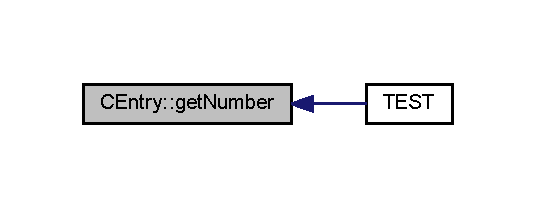
\includegraphics[width=257pt]{class_c_entry_a6e8cde8d4a78cc65fceeb5f0430a2b55_icgraph}
\end{center}
\end{figure}
\mbox{\Hypertarget{class_c_entry_aede4d6e03efa3abb0ed56349edb5b86d}\label{class_c_entry_aede4d6e03efa3abb0ed56349edb5b86d}} 
\index{C\+Entry@{C\+Entry}!get\+Symbol@{get\+Symbol}}
\index{get\+Symbol@{get\+Symbol}!C\+Entry@{C\+Entry}}
\subsubsection{\texorpdfstring{get\+Symbol()}{getSymbol()}}
{\footnotesize\ttfamily const std\+::string \& C\+Entry\+::get\+Symbol (\begin{DoxyParamCaption}{ }\end{DoxyParamCaption}) const}

Getter \begin{DoxyReturn}{Rückgabe}
Bekannte Zeichenkette 
\end{DoxyReturn}
Hier ist ein Graph der zeigt, wo diese Funktion aufgerufen wird\+:
\nopagebreak
\begin{figure}[H]
\begin{center}
\leavevmode
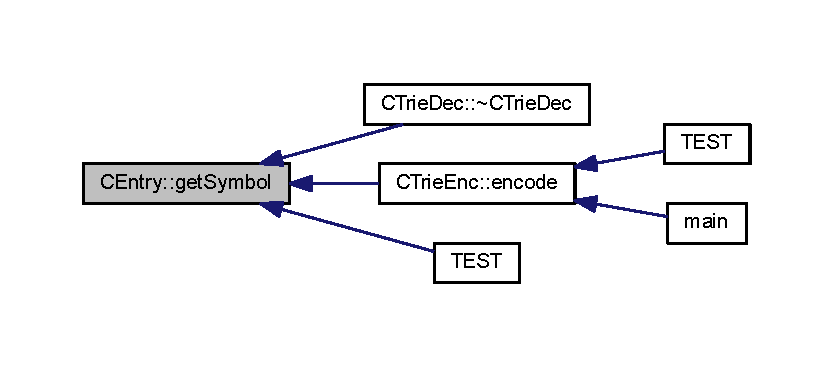
\includegraphics[width=350pt]{class_c_entry_aede4d6e03efa3abb0ed56349edb5b86d_icgraph}
\end{center}
\end{figure}
\mbox{\Hypertarget{class_c_entry_a2ac2cbee24817ff5b67e09f03a952e77}\label{class_c_entry_a2ac2cbee24817ff5b67e09f03a952e77}} 
\index{C\+Entry@{C\+Entry}!set\+Symbol@{set\+Symbol}}
\index{set\+Symbol@{set\+Symbol}!C\+Entry@{C\+Entry}}
\subsubsection{\texorpdfstring{set\+Symbol()}{setSymbol()}}
{\footnotesize\ttfamily void C\+Entry\+::set\+Symbol (\begin{DoxyParamCaption}\item[{std\+::string}]{symbol }\end{DoxyParamCaption})}

Setter 
\begin{DoxyParams}{Parameter}
{\em symbol} & Bekannte Zeichenkette \\
\hline
\end{DoxyParams}
Hier ist ein Graph der zeigt, wo diese Funktion aufgerufen wird\+:
\nopagebreak
\begin{figure}[H]
\begin{center}
\leavevmode
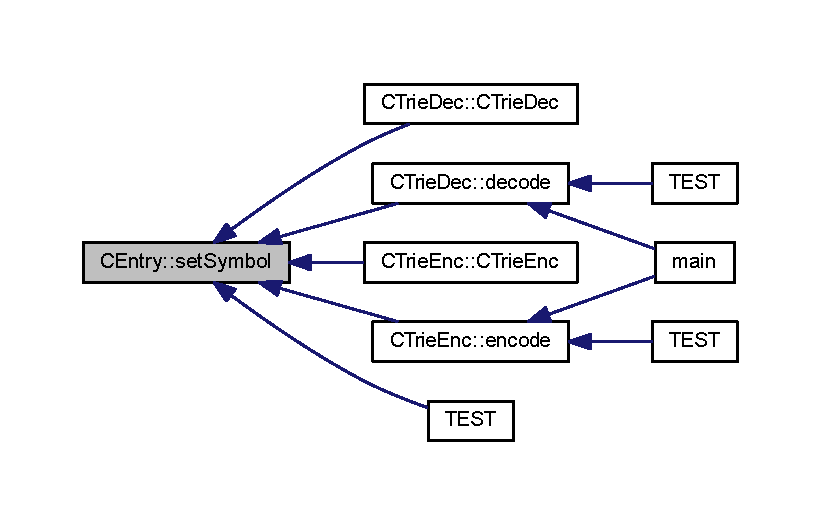
\includegraphics[width=350pt]{class_c_entry_a2ac2cbee24817ff5b67e09f03a952e77_icgraph}
\end{center}
\end{figure}


Die Dokumentation für diese Klasse wurde erzeugt aufgrund der Dateien\+:\begin{DoxyCompactItemize}
\item 
C\+:/portable\+Dev\+Env\+\_\+2017/workspace2017/project/src/\hyperlink{_c_entry_8hpp}{C\+Entry.\+hpp}\item 
C\+:/portable\+Dev\+Env\+\_\+2017/workspace2017/project/src/\hyperlink{_c_entry_8cpp}{C\+Entry.\+cpp}\end{DoxyCompactItemize}

\hypertarget{class_c_forward_counter}{}\section{C\+Forward\+Counter Klassenreferenz}
\label{class_c_forward_counter}\index{C\+Forward\+Counter@{C\+Forward\+Counter}}


{\ttfamily \#include $<$C\+Forward\+Counter.\+hpp$>$}



Klassendiagramm für C\+Forward\+Counter\+:
\nopagebreak
\begin{figure}[H]
\begin{center}
\leavevmode
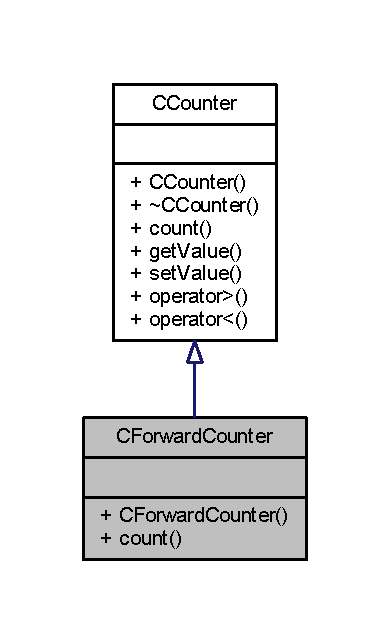
\includegraphics[width=187pt]{class_c_forward_counter__inherit__graph}
\end{center}
\end{figure}


Zusammengehörigkeiten von C\+Forward\+Counter\+:
\nopagebreak
\begin{figure}[H]
\begin{center}
\leavevmode
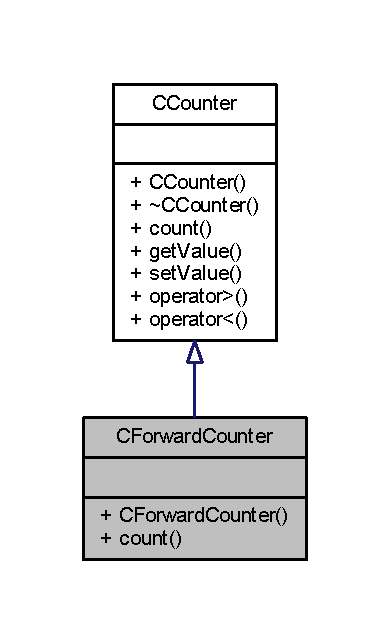
\includegraphics[width=187pt]{class_c_forward_counter__coll__graph}
\end{center}
\end{figure}
\subsection*{Öffentliche Methoden}
\begin{DoxyCompactItemize}
\item 
\hyperlink{class_c_forward_counter_aeda1b05d715820f61e377a2c6fa52b2e}{C\+Forward\+Counter} ()
\item 
void \hyperlink{class_c_forward_counter_afc451afa9f8b76f70b28c08982265a86}{count} ()
\end{DoxyCompactItemize}


\subsection{Ausführliche Beschreibung}
\hyperlink{class_c_forward_counter}{C\+Forward\+Counter}, überschreibt die Memberfunktion \hyperlink{class_c_forward_counter_afc451afa9f8b76f70b28c08982265a86}{count()} aus Basisklasse \hyperlink{class_c_counter}{C\+Counter}, so dass diese den internen Zählerstand um 1 inkrementiert. 

\subsection{Beschreibung der Konstruktoren und Destruktoren}
\mbox{\Hypertarget{class_c_forward_counter_aeda1b05d715820f61e377a2c6fa52b2e}\label{class_c_forward_counter_aeda1b05d715820f61e377a2c6fa52b2e}} 
\index{C\+Forward\+Counter@{C\+Forward\+Counter}!C\+Forward\+Counter@{C\+Forward\+Counter}}
\index{C\+Forward\+Counter@{C\+Forward\+Counter}!C\+Forward\+Counter@{C\+Forward\+Counter}}
\subsubsection{\texorpdfstring{C\+Forward\+Counter()}{CForwardCounter()}}
{\footnotesize\ttfamily C\+Forward\+Counter\+::\+C\+Forward\+Counter (\begin{DoxyParamCaption}{ }\end{DoxyParamCaption})}

Parameterloser Konstruktor, setzt den Zählerstand auf 0 

\subsection{Dokumentation der Elementfunktionen}
\mbox{\Hypertarget{class_c_forward_counter_afc451afa9f8b76f70b28c08982265a86}\label{class_c_forward_counter_afc451afa9f8b76f70b28c08982265a86}} 
\index{C\+Forward\+Counter@{C\+Forward\+Counter}!count@{count}}
\index{count@{count}!C\+Forward\+Counter@{C\+Forward\+Counter}}
\subsubsection{\texorpdfstring{count()}{count()}}
{\footnotesize\ttfamily void C\+Forward\+Counter\+::count (\begin{DoxyParamCaption}{ }\end{DoxyParamCaption})\hspace{0.3cm}{\ttfamily [virtual]}}

Zähler, inkrementiert den Zählerstand um 1 

Erneute Implementation von \hyperlink{class_c_counter_a90f3e164f3fc1dcf91044702d6940c4d}{C\+Counter}.

Hier ist ein Graph der zeigt, wo diese Funktion aufgerufen wird\+:
\nopagebreak
\begin{figure}[H]
\begin{center}
\leavevmode
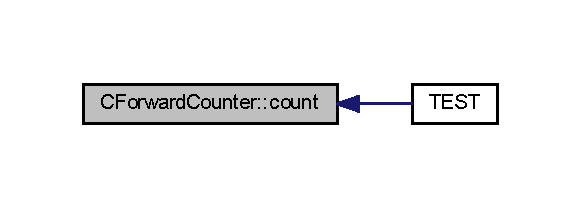
\includegraphics[width=279pt]{class_c_forward_counter_afc451afa9f8b76f70b28c08982265a86_icgraph}
\end{center}
\end{figure}


Die Dokumentation für diese Klasse wurde erzeugt aufgrund der Dateien\+:\begin{DoxyCompactItemize}
\item 
C\+:/portable\+Dev\+Env\+\_\+2017/workspace2017/\+Blatt2/src/\hyperlink{_c_forward_counter_8hpp}{C\+Forward\+Counter.\+hpp}\item 
C\+:/portable\+Dev\+Env\+\_\+2017/workspace2017/\+Blatt2/src/\hyperlink{_c_forward_counter_8cpp}{C\+Forward\+Counter.\+cpp}\end{DoxyCompactItemize}

\hypertarget{class_c_knot}{}\section{C\+Knot Klassenreferenz}
\label{class_c_knot}\index{C\+Knot@{C\+Knot}}


Erweiterung von \hyperlink{class_c_entry}{C\+Entry} Erweitert \hyperlink{class_c_entry}{C\+Entry} zusätzlich um die Variable m\+\_\+parent und wird zur Verwaltung bisher bekannter Zeichenketten verwendet.  




{\ttfamily \#include $<$C\+Knot.\+hpp$>$}



Klassendiagramm für C\+Knot\+:
\nopagebreak
\begin{figure}[H]
\begin{center}
\leavevmode
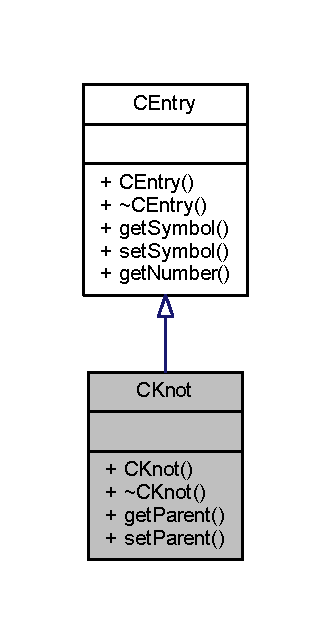
\includegraphics[width=159pt]{class_c_knot__inherit__graph}
\end{center}
\end{figure}


Zusammengehörigkeiten von C\+Knot\+:
\nopagebreak
\begin{figure}[H]
\begin{center}
\leavevmode
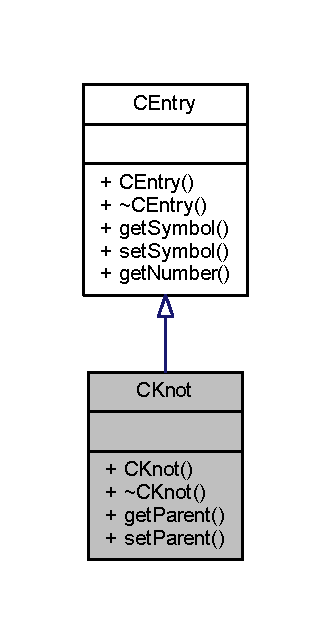
\includegraphics[width=159pt]{class_c_knot__coll__graph}
\end{center}
\end{figure}
\subsection*{Öffentliche Methoden}
\begin{DoxyCompactItemize}
\item 
\hyperlink{class_c_knot_aebedf7efb952e68b564b0e56300e8135}{C\+Knot} ()
\item 
virtual \hyperlink{class_c_knot_a8752f1fc4c060fa291a850c9c36889e1}{$\sim$\+C\+Knot} ()
\item 
int \hyperlink{class_c_knot_a22a037af3ea6162ff6d380480d568b80}{get\+Parent} () const
\item 
void \hyperlink{class_c_knot_a6ad905f6be13af0bdff157559c02b909}{set\+Parent} (int parent)
\end{DoxyCompactItemize}
\subsection*{Weitere Geerbte Elemente}


\subsection{Ausführliche Beschreibung}
Erweiterung von \hyperlink{class_c_entry}{C\+Entry} Erweitert \hyperlink{class_c_entry}{C\+Entry} zusätzlich um die Variable m\+\_\+parent und wird zur Verwaltung bisher bekannter Zeichenketten verwendet. 

\subsection{Beschreibung der Konstruktoren und Destruktoren}
\mbox{\Hypertarget{class_c_knot_aebedf7efb952e68b564b0e56300e8135}\label{class_c_knot_aebedf7efb952e68b564b0e56300e8135}} 
\index{C\+Knot@{C\+Knot}!C\+Knot@{C\+Knot}}
\index{C\+Knot@{C\+Knot}!C\+Knot@{C\+Knot}}
\subsubsection{\texorpdfstring{C\+Knot()}{CKnot()}}
{\footnotesize\ttfamily C\+Knot\+::\+C\+Knot (\begin{DoxyParamCaption}{ }\end{DoxyParamCaption})}

Parameterloser Konstruktor \mbox{\Hypertarget{class_c_knot_a8752f1fc4c060fa291a850c9c36889e1}\label{class_c_knot_a8752f1fc4c060fa291a850c9c36889e1}} 
\index{C\+Knot@{C\+Knot}!````~C\+Knot@{$\sim$\+C\+Knot}}
\index{````~C\+Knot@{$\sim$\+C\+Knot}!C\+Knot@{C\+Knot}}
\subsubsection{\texorpdfstring{$\sim$\+C\+Knot()}{~CKnot()}}
{\footnotesize\ttfamily C\+Knot\+::$\sim$\+C\+Knot (\begin{DoxyParamCaption}{ }\end{DoxyParamCaption})\hspace{0.3cm}{\ttfamily [virtual]}}

Destruktor 

\subsection{Dokumentation der Elementfunktionen}
\mbox{\Hypertarget{class_c_knot_a22a037af3ea6162ff6d380480d568b80}\label{class_c_knot_a22a037af3ea6162ff6d380480d568b80}} 
\index{C\+Knot@{C\+Knot}!get\+Parent@{get\+Parent}}
\index{get\+Parent@{get\+Parent}!C\+Knot@{C\+Knot}}
\subsubsection{\texorpdfstring{get\+Parent()}{getParent()}}
{\footnotesize\ttfamily int C\+Knot\+::get\+Parent (\begin{DoxyParamCaption}{ }\end{DoxyParamCaption}) const}

Getter \begin{DoxyReturn}{Rückgabe}
Adresse des übergeodneten Knotens (Parent) 
\end{DoxyReturn}
Hier ist ein Graph der zeigt, wo diese Funktion aufgerufen wird\+:
\nopagebreak
\begin{figure}[H]
\begin{center}
\leavevmode
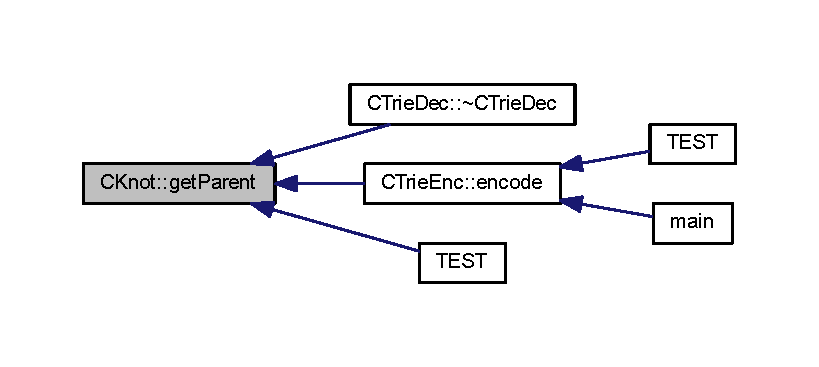
\includegraphics[width=350pt]{class_c_knot_a22a037af3ea6162ff6d380480d568b80_icgraph}
\end{center}
\end{figure}
\mbox{\Hypertarget{class_c_knot_a6ad905f6be13af0bdff157559c02b909}\label{class_c_knot_a6ad905f6be13af0bdff157559c02b909}} 
\index{C\+Knot@{C\+Knot}!set\+Parent@{set\+Parent}}
\index{set\+Parent@{set\+Parent}!C\+Knot@{C\+Knot}}
\subsubsection{\texorpdfstring{set\+Parent()}{setParent()}}
{\footnotesize\ttfamily void C\+Knot\+::set\+Parent (\begin{DoxyParamCaption}\item[{int}]{parent }\end{DoxyParamCaption})}

Setter 
\begin{DoxyParams}{Parameter}
{\em parent} & neue Adresse des übergeodneten Knotens (Parent) \\
\hline
\end{DoxyParams}
Hier ist ein Graph der zeigt, wo diese Funktion aufgerufen wird\+:
\nopagebreak
\begin{figure}[H]
\begin{center}
\leavevmode
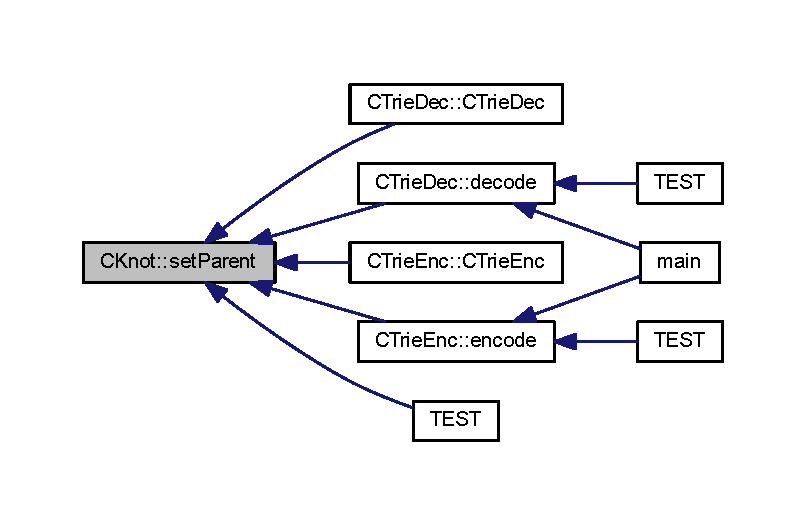
\includegraphics[width=350pt]{class_c_knot_a6ad905f6be13af0bdff157559c02b909_icgraph}
\end{center}
\end{figure}


Die Dokumentation für diese Klasse wurde erzeugt aufgrund der Dateien\+:\begin{DoxyCompactItemize}
\item 
C\+:/portable\+Dev\+Env\+\_\+2017/workspace2017/project/src/\hyperlink{_c_knot_8hpp}{C\+Knot.\+hpp}\item 
C\+:/portable\+Dev\+Env\+\_\+2017/workspace2017/project/src/\hyperlink{_c_knot_8cpp}{C\+Knot.\+cpp}\end{DoxyCompactItemize}

\hypertarget{class_c_l_z_w}{}\section{C\+L\+ZW Klassenreferenz}
\label{class_c_l_z_w}\index{C\+L\+ZW@{C\+L\+ZW}}


\hyperlink{_c_l_z_w_8hpp}{C\+L\+Z\+W.\+hpp} Basisklasse für L\+ZW Encoder und Decoder.  




{\ttfamily \#include $<$C\+L\+Z\+W.\+hpp$>$}



Klassendiagramm für C\+L\+ZW\+:
\nopagebreak
\begin{figure}[H]
\begin{center}
\leavevmode
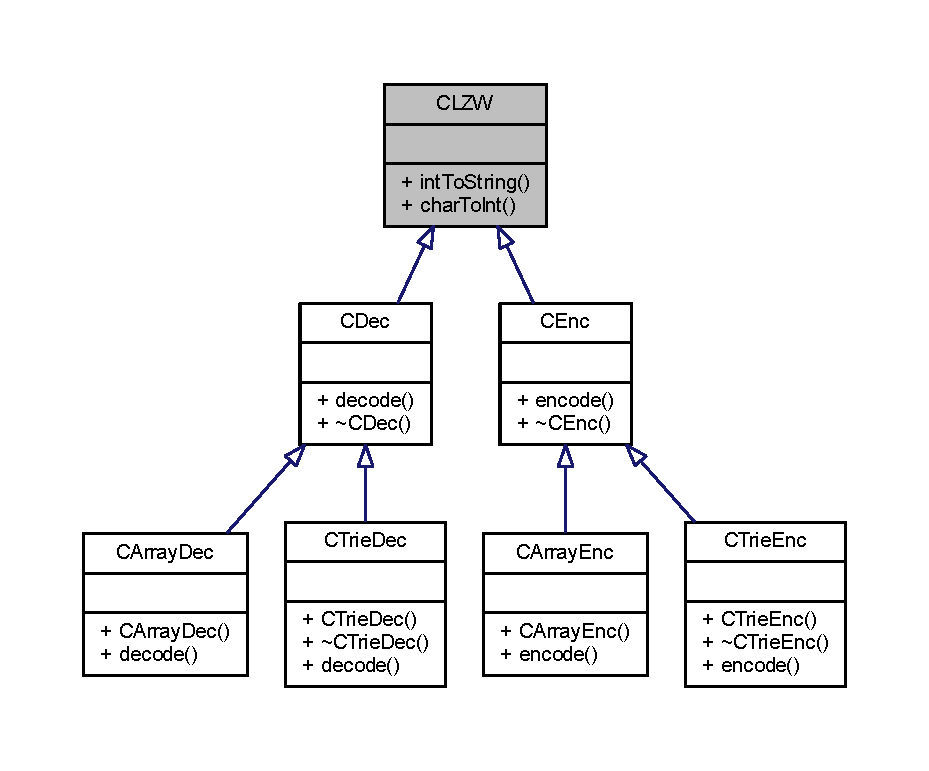
\includegraphics[width=350pt]{class_c_l_z_w__inherit__graph}
\end{center}
\end{figure}


Zusammengehörigkeiten von C\+L\+ZW\+:
\nopagebreak
\begin{figure}[H]
\begin{center}
\leavevmode
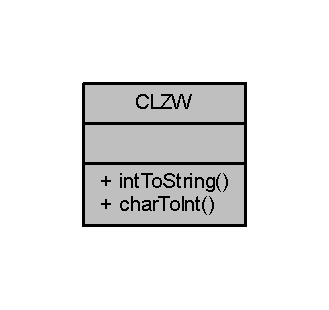
\includegraphics[width=158pt]{class_c_l_z_w__coll__graph}
\end{center}
\end{figure}
\subsection*{Öffentliche, statische Methoden}
\begin{DoxyCompactItemize}
\item 
static string \hyperlink{class_c_l_z_w_a7cd7b5a245b1b3a0eb1905d3a8e2be89}{int\+To\+String} (int i)
\item 
static unsigned int \hyperlink{class_c_l_z_w_ad7b0dd957592e723dea646d3e02771aa}{char\+To\+Int} (char)
\end{DoxyCompactItemize}


\subsection{Ausführliche Beschreibung}
\hyperlink{_c_l_z_w_8hpp}{C\+L\+Z\+W.\+hpp} Basisklasse für L\+ZW Encoder und Decoder. 

int\+To\+String ermöglicht das Umwandeln von Integern zu string char\+To\+Int ermöglicht das Umwandeln von einzelnen Elementen eines string in die zugehörige A\+S\+C\+I\+I-\/\+Zahl auch für Einträge 128-\/255 (z.\+B. Umlaute) 

\subsection{Dokumentation der Elementfunktionen}
\mbox{\Hypertarget{class_c_l_z_w_ad7b0dd957592e723dea646d3e02771aa}\label{class_c_l_z_w_ad7b0dd957592e723dea646d3e02771aa}} 
\index{C\+L\+ZW@{C\+L\+ZW}!char\+To\+Int@{char\+To\+Int}}
\index{char\+To\+Int@{char\+To\+Int}!C\+L\+ZW@{C\+L\+ZW}}
\subsubsection{\texorpdfstring{char\+To\+Int()}{charToInt()}}
{\footnotesize\ttfamily unsigned int C\+L\+Z\+W\+::char\+To\+Int (\begin{DoxyParamCaption}\item[{char}]{in\+Char }\end{DoxyParamCaption})\hspace{0.3cm}{\ttfamily [static]}}

Hier ist ein Graph der zeigt, wo diese Funktion aufgerufen wird\+:
\nopagebreak
\begin{figure}[H]
\begin{center}
\leavevmode
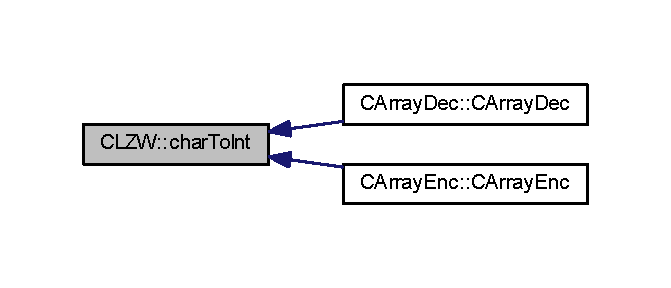
\includegraphics[width=322pt]{class_c_l_z_w_ad7b0dd957592e723dea646d3e02771aa_icgraph}
\end{center}
\end{figure}
\mbox{\Hypertarget{class_c_l_z_w_a7cd7b5a245b1b3a0eb1905d3a8e2be89}\label{class_c_l_z_w_a7cd7b5a245b1b3a0eb1905d3a8e2be89}} 
\index{C\+L\+ZW@{C\+L\+ZW}!int\+To\+String@{int\+To\+String}}
\index{int\+To\+String@{int\+To\+String}!C\+L\+ZW@{C\+L\+ZW}}
\subsubsection{\texorpdfstring{int\+To\+String()}{intToString()}}
{\footnotesize\ttfamily string C\+L\+Z\+W\+::int\+To\+String (\begin{DoxyParamCaption}\item[{int}]{i }\end{DoxyParamCaption})\hspace{0.3cm}{\ttfamily [static]}}

Hier ist ein Graph der zeigt, wo diese Funktion aufgerufen wird\+:
\nopagebreak
\begin{figure}[H]
\begin{center}
\leavevmode
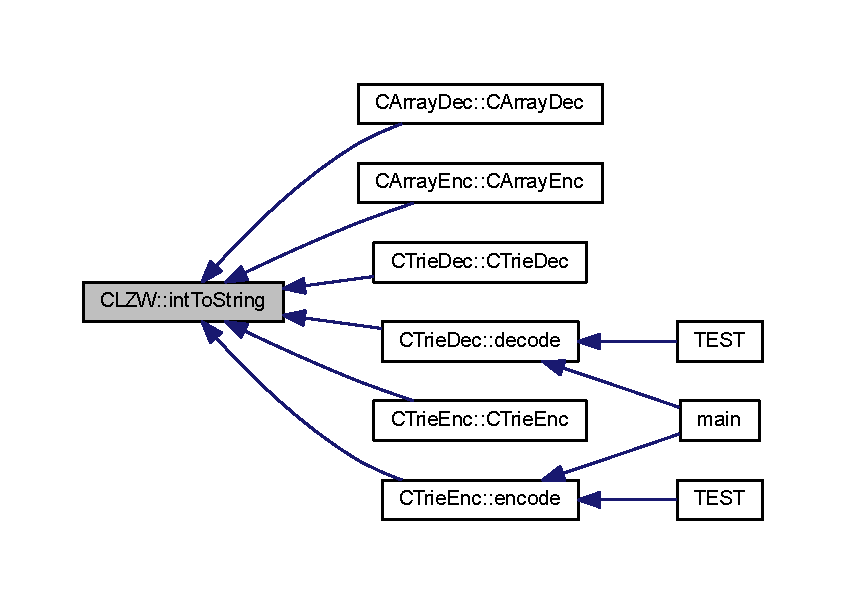
\includegraphics[width=350pt]{class_c_l_z_w_a7cd7b5a245b1b3a0eb1905d3a8e2be89_icgraph}
\end{center}
\end{figure}


Die Dokumentation für diese Klasse wurde erzeugt aufgrund der Dateien\+:\begin{DoxyCompactItemize}
\item 
C\+:/portable\+Dev\+Env\+\_\+2017/workspace2017/project/src/\hyperlink{_c_l_z_w_8hpp}{C\+L\+Z\+W.\+hpp}\item 
C\+:/portable\+Dev\+Env\+\_\+2017/workspace2017/project/src/\hyperlink{_c_l_z_w_8cpp}{C\+L\+Z\+W.\+cpp}\end{DoxyCompactItemize}

\hypertarget{class_c_trie_dec}{}\section{C\+Trie\+Dec Klassenreferenz}
\label{class_c_trie_dec}\index{C\+Trie\+Dec@{C\+Trie\+Dec}}


L\+ZW Decoder Klasse für die Decodierung erbt von \hyperlink{class_c_enc}{C\+Enc}.  




{\ttfamily \#include $<$C\+Trie\+Dec.\+hpp$>$}



Klassendiagramm für C\+Trie\+Dec\+:
\nopagebreak
\begin{figure}[H]
\begin{center}
\leavevmode
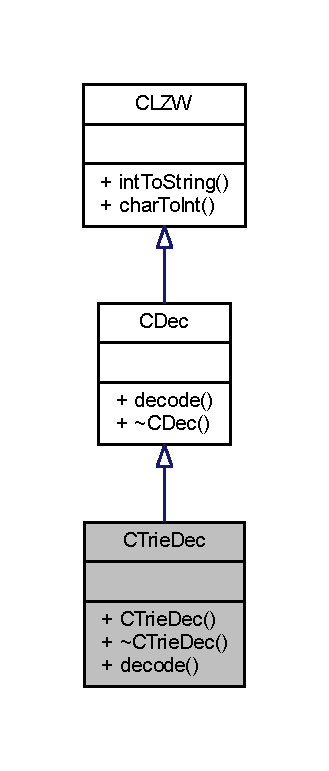
\includegraphics[width=158pt]{class_c_trie_dec__inherit__graph}
\end{center}
\end{figure}


Zusammengehörigkeiten von C\+Trie\+Dec\+:
\nopagebreak
\begin{figure}[H]
\begin{center}
\leavevmode
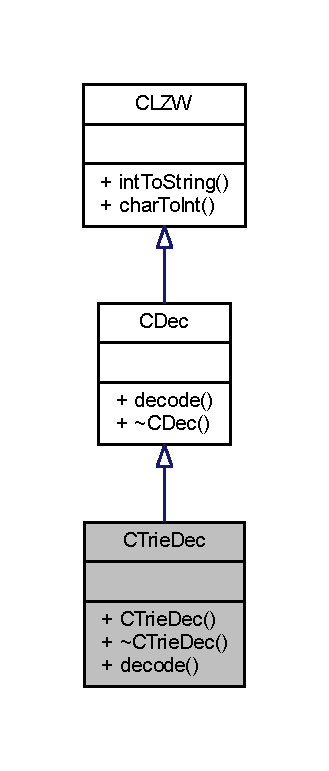
\includegraphics[width=158pt]{class_c_trie_dec__coll__graph}
\end{center}
\end{figure}
\subsection*{Öffentliche Methoden}
\begin{DoxyCompactItemize}
\item 
\hyperlink{class_c_trie_dec_a64323697e83419686801b04c5b12ac37}{C\+Trie\+Dec} ()
\item 
\hyperlink{class_c_trie_dec_a2e3dee1b9fae4e8fd82a7ba6247bb564}{$\sim$\+C\+Trie\+Dec} ()
\item 
std\+::string \hyperlink{class_c_trie_dec_a190f82222a2f7881b940066c54b00d38}{decode} (const std\+::vector$<$ unsigned int $>$ \&enc)
\end{DoxyCompactItemize}
\subsection*{Weitere Geerbte Elemente}


\subsection{Ausführliche Beschreibung}
L\+ZW Decoder Klasse für die Decodierung erbt von \hyperlink{class_c_enc}{C\+Enc}. 

\subsection{Beschreibung der Konstruktoren und Destruktoren}
\mbox{\Hypertarget{class_c_trie_dec_a64323697e83419686801b04c5b12ac37}\label{class_c_trie_dec_a64323697e83419686801b04c5b12ac37}} 
\index{C\+Trie\+Dec@{C\+Trie\+Dec}!C\+Trie\+Dec@{C\+Trie\+Dec}}
\index{C\+Trie\+Dec@{C\+Trie\+Dec}!C\+Trie\+Dec@{C\+Trie\+Dec}}
\subsubsection{\texorpdfstring{C\+Trie\+Dec()}{CTrieDec()}}
{\footnotesize\ttfamily C\+Trie\+Dec\+::\+C\+Trie\+Dec (\begin{DoxyParamCaption}{ }\end{DoxyParamCaption})}

Paramenterloser Konstruktor der Klasse Initialisiert das Dictionary Hier ist ein Graph, der zeigt, was diese Funktion aufruft\+:
\nopagebreak
\begin{figure}[H]
\begin{center}
\leavevmode
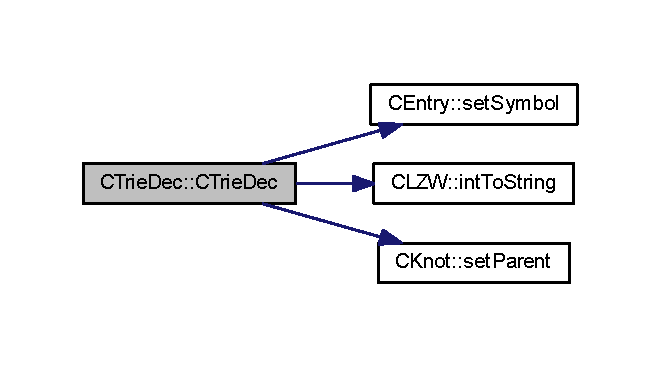
\includegraphics[width=317pt]{class_c_trie_dec_a64323697e83419686801b04c5b12ac37_cgraph}
\end{center}
\end{figure}
\mbox{\Hypertarget{class_c_trie_dec_a2e3dee1b9fae4e8fd82a7ba6247bb564}\label{class_c_trie_dec_a2e3dee1b9fae4e8fd82a7ba6247bb564}} 
\index{C\+Trie\+Dec@{C\+Trie\+Dec}!````~C\+Trie\+Dec@{$\sim$\+C\+Trie\+Dec}}
\index{````~C\+Trie\+Dec@{$\sim$\+C\+Trie\+Dec}!C\+Trie\+Dec@{C\+Trie\+Dec}}
\subsubsection{\texorpdfstring{$\sim$\+C\+Trie\+Dec()}{~CTrieDec()}}
{\footnotesize\ttfamily C\+Trie\+Dec\+::$\sim$\+C\+Trie\+Dec (\begin{DoxyParamCaption}{ }\end{DoxyParamCaption})}

Destruktor Hier ist ein Graph, der zeigt, was diese Funktion aufruft\+:
\nopagebreak
\begin{figure}[H]
\begin{center}
\leavevmode
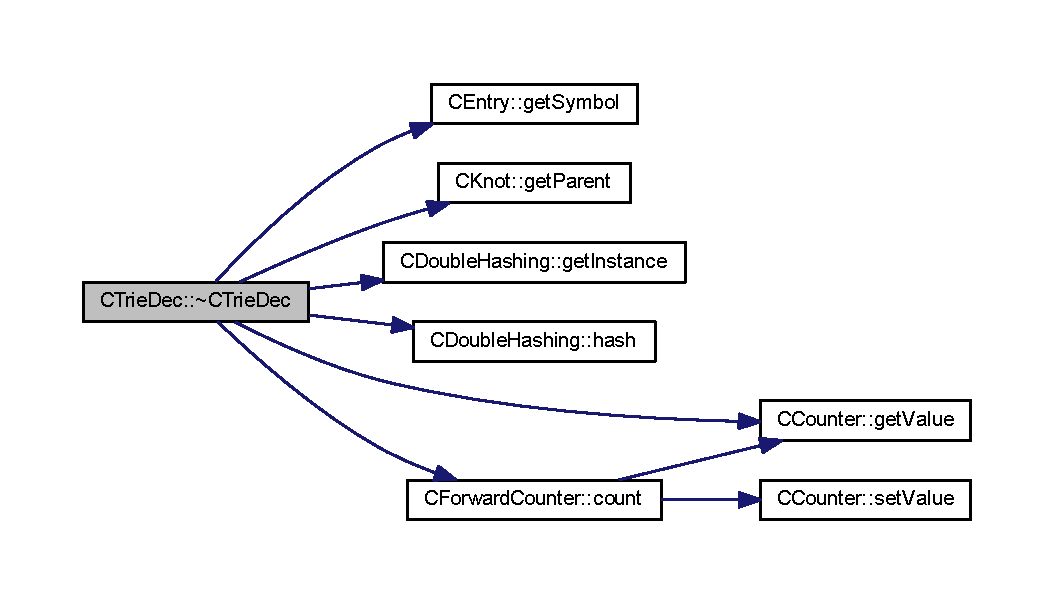
\includegraphics[width=350pt]{class_c_trie_dec_a2e3dee1b9fae4e8fd82a7ba6247bb564_cgraph}
\end{center}
\end{figure}


\subsection{Dokumentation der Elementfunktionen}
\mbox{\Hypertarget{class_c_trie_dec_a190f82222a2f7881b940066c54b00d38}\label{class_c_trie_dec_a190f82222a2f7881b940066c54b00d38}} 
\index{C\+Trie\+Dec@{C\+Trie\+Dec}!decode@{decode}}
\index{decode@{decode}!C\+Trie\+Dec@{C\+Trie\+Dec}}
\subsubsection{\texorpdfstring{decode()}{decode()}}
{\footnotesize\ttfamily std\+::string C\+Trie\+Dec\+::decode (\begin{DoxyParamCaption}\item[{const std\+::vector$<$ unsigned int $>$ \&}]{enc }\end{DoxyParamCaption})}

L\+ZW decoder-\/function 
\begin{DoxyParams}{Parameter}
{\em enc} & komprimierte Zeichenkette als vector \\
\hline
\end{DoxyParams}
\begin{DoxyReturn}{Rückgabe}
Enschlüsselte Zeichenkette 
\end{DoxyReturn}
Hier ist ein Graph, der zeigt, was diese Funktion aufruft\+:
\nopagebreak
\begin{figure}[H]
\begin{center}
\leavevmode
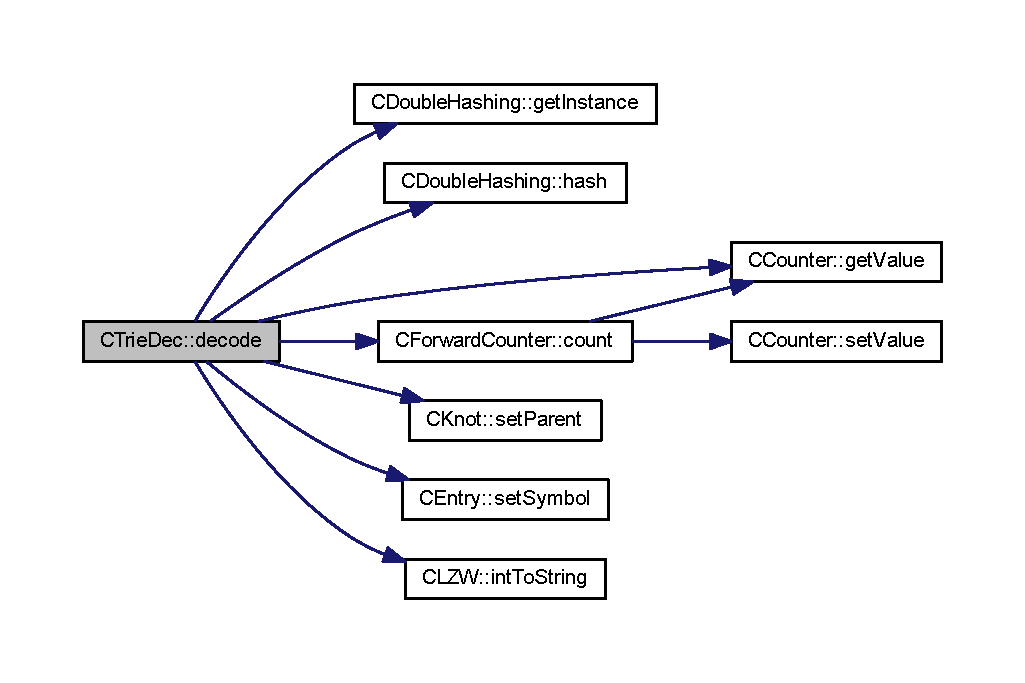
\includegraphics[width=350pt]{class_c_trie_dec_a190f82222a2f7881b940066c54b00d38_cgraph}
\end{center}
\end{figure}
Hier ist ein Graph der zeigt, wo diese Funktion aufgerufen wird\+:
\nopagebreak
\begin{figure}[H]
\begin{center}
\leavevmode
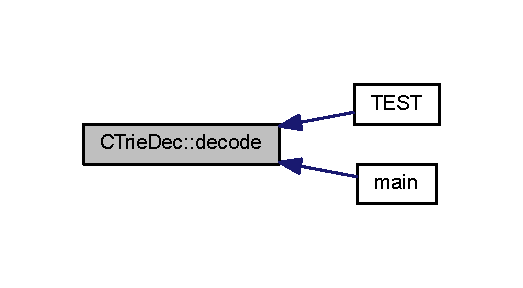
\includegraphics[width=251pt]{class_c_trie_dec_a190f82222a2f7881b940066c54b00d38_icgraph}
\end{center}
\end{figure}


Die Dokumentation für diese Klasse wurde erzeugt aufgrund der Dateien\+:\begin{DoxyCompactItemize}
\item 
C\+:/portable\+Dev\+Env\+\_\+2017/workspace2017/project/src/\hyperlink{_c_trie_dec_8hpp}{C\+Trie\+Dec.\+hpp}\item 
C\+:/portable\+Dev\+Env\+\_\+2017/workspace2017/project/src/\hyperlink{_c_trie_dec_8cpp}{C\+Trie\+Dec.\+cpp}\end{DoxyCompactItemize}

\hypertarget{class_c_trie_enc}{}\section{C\+Trie\+Enc Klassenreferenz}
\label{class_c_trie_enc}\index{C\+Trie\+Enc@{C\+Trie\+Enc}}


L\+ZW Encoder Klasse für die Encodierung erbt von \hyperlink{class_c_enc}{C\+Enc}.  




{\ttfamily \#include $<$C\+Trie\+Enc.\+hpp$>$}



Klassendiagramm für C\+Trie\+Enc\+:
\nopagebreak
\begin{figure}[H]
\begin{center}
\leavevmode
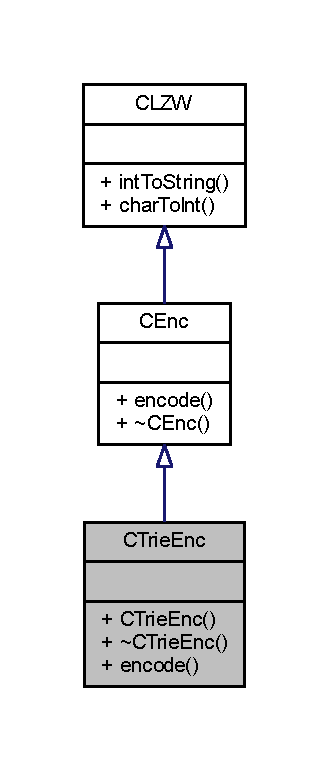
\includegraphics[width=158pt]{class_c_trie_enc__inherit__graph}
\end{center}
\end{figure}


Zusammengehörigkeiten von C\+Trie\+Enc\+:
\nopagebreak
\begin{figure}[H]
\begin{center}
\leavevmode
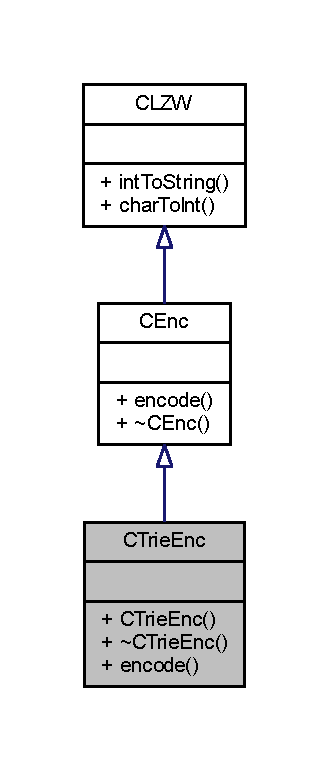
\includegraphics[width=158pt]{class_c_trie_enc__coll__graph}
\end{center}
\end{figure}
\subsection*{Öffentliche Methoden}
\begin{DoxyCompactItemize}
\item 
\hyperlink{class_c_trie_enc_ace11a48f0a8dab419a410b61cb58cfdc}{C\+Trie\+Enc} ()
\item 
\hyperlink{class_c_trie_enc_a6627940420ef4052bd8d395db959b562}{$\sim$\+C\+Trie\+Enc} ()
\item 
std\+::vector$<$ unsigned int $>$ \hyperlink{class_c_trie_enc_a14832d9694f7aa5ba9d7d32d3a3c0793}{encode} (const std\+::string \&in)
\end{DoxyCompactItemize}
\subsection*{Weitere Geerbte Elemente}


\subsection{Ausführliche Beschreibung}
L\+ZW Encoder Klasse für die Encodierung erbt von \hyperlink{class_c_enc}{C\+Enc}. 

\subsection{Beschreibung der Konstruktoren und Destruktoren}
\mbox{\Hypertarget{class_c_trie_enc_ace11a48f0a8dab419a410b61cb58cfdc}\label{class_c_trie_enc_ace11a48f0a8dab419a410b61cb58cfdc}} 
\index{C\+Trie\+Enc@{C\+Trie\+Enc}!C\+Trie\+Enc@{C\+Trie\+Enc}}
\index{C\+Trie\+Enc@{C\+Trie\+Enc}!C\+Trie\+Enc@{C\+Trie\+Enc}}
\subsubsection{\texorpdfstring{C\+Trie\+Enc()}{CTrieEnc()}}
{\footnotesize\ttfamily C\+Trie\+Enc\+::\+C\+Trie\+Enc (\begin{DoxyParamCaption}{ }\end{DoxyParamCaption})}

Paramenterloser Konstruktor der Klasse Initialisiert das Dictionary Hier ist ein Graph, der zeigt, was diese Funktion aufruft\+:
\nopagebreak
\begin{figure}[H]
\begin{center}
\leavevmode
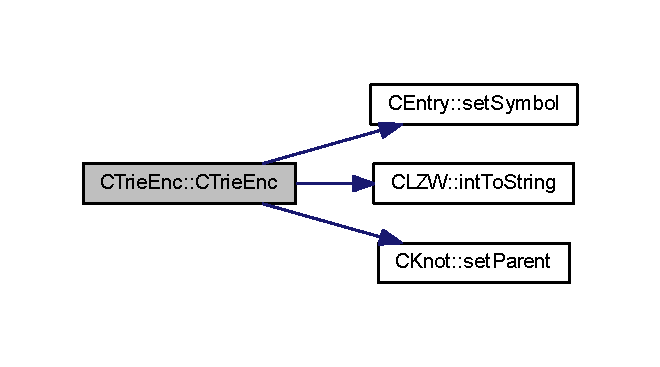
\includegraphics[width=317pt]{class_c_trie_enc_ace11a48f0a8dab419a410b61cb58cfdc_cgraph}
\end{center}
\end{figure}
\mbox{\Hypertarget{class_c_trie_enc_a6627940420ef4052bd8d395db959b562}\label{class_c_trie_enc_a6627940420ef4052bd8d395db959b562}} 
\index{C\+Trie\+Enc@{C\+Trie\+Enc}!````~C\+Trie\+Enc@{$\sim$\+C\+Trie\+Enc}}
\index{````~C\+Trie\+Enc@{$\sim$\+C\+Trie\+Enc}!C\+Trie\+Enc@{C\+Trie\+Enc}}
\subsubsection{\texorpdfstring{$\sim$\+C\+Trie\+Enc()}{~CTrieEnc()}}
{\footnotesize\ttfamily C\+Trie\+Enc\+::$\sim$\+C\+Trie\+Enc (\begin{DoxyParamCaption}{ }\end{DoxyParamCaption})}



\subsection{Dokumentation der Elementfunktionen}
\mbox{\Hypertarget{class_c_trie_enc_a14832d9694f7aa5ba9d7d32d3a3c0793}\label{class_c_trie_enc_a14832d9694f7aa5ba9d7d32d3a3c0793}} 
\index{C\+Trie\+Enc@{C\+Trie\+Enc}!encode@{encode}}
\index{encode@{encode}!C\+Trie\+Enc@{C\+Trie\+Enc}}
\subsubsection{\texorpdfstring{encode()}{encode()}}
{\footnotesize\ttfamily std\+::vector$<$ unsigned int $>$ C\+Trie\+Enc\+::encode (\begin{DoxyParamCaption}\item[{const std\+::string \&}]{in }\end{DoxyParamCaption})}

L\+ZW encoder-\/function 
\begin{DoxyParams}{Parameter}
{\em in} & zu komprimierende Zeichenkette \\
\hline
\end{DoxyParams}
\begin{DoxyReturn}{Rückgabe}
kompimierte Zeichenkette als vector 
\end{DoxyReturn}
Hier ist ein Graph, der zeigt, was diese Funktion aufruft\+:
\nopagebreak
\begin{figure}[H]
\begin{center}
\leavevmode
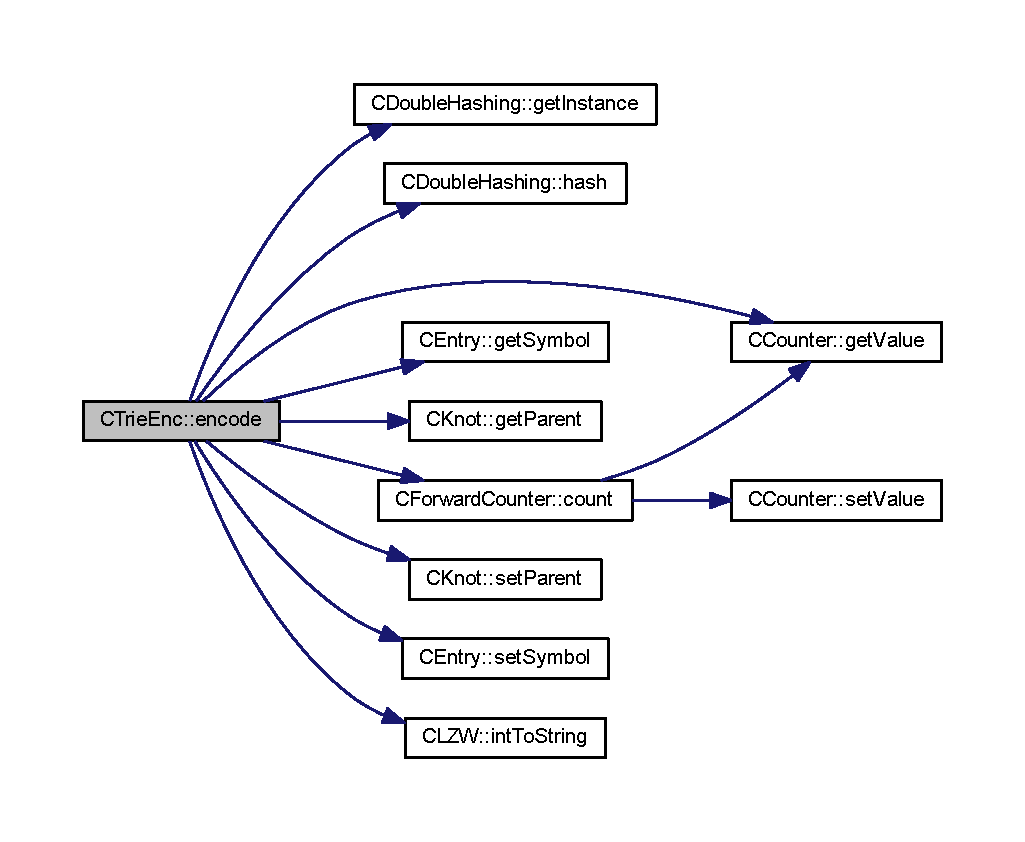
\includegraphics[width=350pt]{class_c_trie_enc_a14832d9694f7aa5ba9d7d32d3a3c0793_cgraph}
\end{center}
\end{figure}
Hier ist ein Graph der zeigt, wo diese Funktion aufgerufen wird\+:
\nopagebreak
\begin{figure}[H]
\begin{center}
\leavevmode
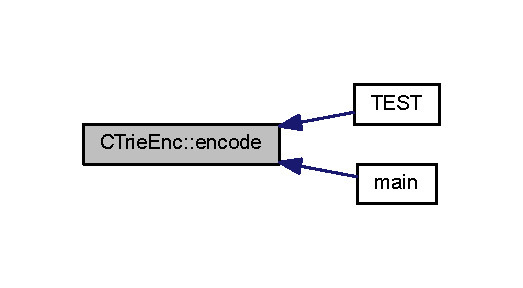
\includegraphics[width=251pt]{class_c_trie_enc_a14832d9694f7aa5ba9d7d32d3a3c0793_icgraph}
\end{center}
\end{figure}


Die Dokumentation für diese Klasse wurde erzeugt aufgrund der Dateien\+:\begin{DoxyCompactItemize}
\item 
C\+:/portable\+Dev\+Env\+\_\+2017/workspace2017/project/src/\hyperlink{_c_trie_enc_8hpp}{C\+Trie\+Enc.\+hpp}\item 
C\+:/portable\+Dev\+Env\+\_\+2017/workspace2017/project/src/\hyperlink{_c_trie_enc_8cpp}{C\+Trie\+Enc.\+cpp}\end{DoxyCompactItemize}

\hypertarget{class_x_out_of_bounds}{}\section{X\+Out\+Of\+Bounds Klassenreferenz}
\label{class_x_out_of_bounds}\index{X\+Out\+Of\+Bounds@{X\+Out\+Of\+Bounds}}


Ausnahmeklasse Abgeleitete Klasse von std\+::exception. Speichert Ausnahmen und gibt diese auch wieder aus.  




{\ttfamily \#include $<$X\+Out\+Of\+Bounds.\+hpp$>$}



Klassendiagramm für X\+Out\+Of\+Bounds\+:
\nopagebreak
\begin{figure}[H]
\begin{center}
\leavevmode
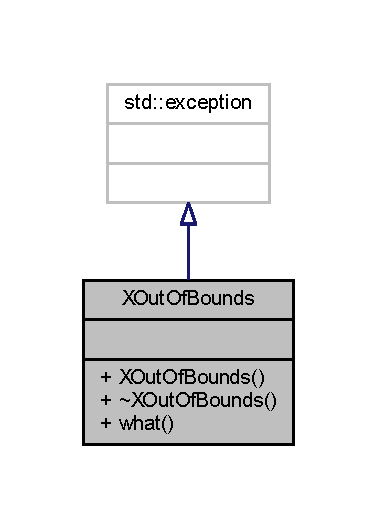
\includegraphics[width=181pt]{class_x_out_of_bounds__inherit__graph}
\end{center}
\end{figure}


Zusammengehörigkeiten von X\+Out\+Of\+Bounds\+:
\nopagebreak
\begin{figure}[H]
\begin{center}
\leavevmode
\includegraphics[width=181pt]{class_x_out_of_bounds__coll__graph}
\end{center}
\end{figure}
\subsection*{Öffentliche Methoden}
\begin{DoxyCompactItemize}
\item 
\hyperlink{class_x_out_of_bounds_a9e2fc4dfa3f25d730563ff2492f40662}{X\+Out\+Of\+Bounds} (const char $\ast$msg)
\item 
virtual \hyperlink{class_x_out_of_bounds_a7655380482ddb2f03570caee39fa2748}{$\sim$\+X\+Out\+Of\+Bounds} ()  throw ()
\item 
const char $\ast$ \hyperlink{class_x_out_of_bounds_a5a047c4fa3db7ef57de7732ae4a2e937}{what} () const  throw ()
\begin{DoxyCompactList}\small\item\em Getter Kann aufgrund von throw() selbst keine exceptions werfen. \end{DoxyCompactList}\end{DoxyCompactItemize}


\subsection{Ausführliche Beschreibung}
Ausnahmeklasse Abgeleitete Klasse von std\+::exception. Speichert Ausnahmen und gibt diese auch wieder aus. 

\subsection{Beschreibung der Konstruktoren und Destruktoren}
\mbox{\Hypertarget{class_x_out_of_bounds_a9e2fc4dfa3f25d730563ff2492f40662}\label{class_x_out_of_bounds_a9e2fc4dfa3f25d730563ff2492f40662}} 
\index{X\+Out\+Of\+Bounds@{X\+Out\+Of\+Bounds}!X\+Out\+Of\+Bounds@{X\+Out\+Of\+Bounds}}
\index{X\+Out\+Of\+Bounds@{X\+Out\+Of\+Bounds}!X\+Out\+Of\+Bounds@{X\+Out\+Of\+Bounds}}
\subsubsection{\texorpdfstring{X\+Out\+Of\+Bounds()}{XOutOfBounds()}}
{\footnotesize\ttfamily X\+Out\+Of\+Bounds\+::\+X\+Out\+Of\+Bounds (\begin{DoxyParamCaption}\item[{const char $\ast$}]{msg }\end{DoxyParamCaption})}

Konstruktor 
\begin{DoxyParams}{Parameter}
{\em msg} & Beschreibung / Bezeichnung der Ausnahme \\
\hline
\end{DoxyParams}
\mbox{\Hypertarget{class_x_out_of_bounds_a7655380482ddb2f03570caee39fa2748}\label{class_x_out_of_bounds_a7655380482ddb2f03570caee39fa2748}} 
\index{X\+Out\+Of\+Bounds@{X\+Out\+Of\+Bounds}!````~X\+Out\+Of\+Bounds@{$\sim$\+X\+Out\+Of\+Bounds}}
\index{````~X\+Out\+Of\+Bounds@{$\sim$\+X\+Out\+Of\+Bounds}!X\+Out\+Of\+Bounds@{X\+Out\+Of\+Bounds}}
\subsubsection{\texorpdfstring{$\sim$\+X\+Out\+Of\+Bounds()}{~XOutOfBounds()}}
{\footnotesize\ttfamily X\+Out\+Of\+Bounds\+::$\sim$\+X\+Out\+Of\+Bounds (\begin{DoxyParamCaption}{ }\end{DoxyParamCaption}) throw  ) \hspace{0.3cm}{\ttfamily [virtual]}}

Destruktor

Kann aufgrund von throw() selbst keine exceptions werfen. 

\subsection{Dokumentation der Elementfunktionen}
\mbox{\Hypertarget{class_x_out_of_bounds_a5a047c4fa3db7ef57de7732ae4a2e937}\label{class_x_out_of_bounds_a5a047c4fa3db7ef57de7732ae4a2e937}} 
\index{X\+Out\+Of\+Bounds@{X\+Out\+Of\+Bounds}!what@{what}}
\index{what@{what}!X\+Out\+Of\+Bounds@{X\+Out\+Of\+Bounds}}
\subsubsection{\texorpdfstring{what()}{what()}}
{\footnotesize\ttfamily const char $\ast$ X\+Out\+Of\+Bounds\+::what (\begin{DoxyParamCaption}{ }\end{DoxyParamCaption}) const throw  ) }



Getter Kann aufgrund von throw() selbst keine exceptions werfen. 

\begin{DoxyReturn}{Rückgabe}
Beschreibung / Bezeichnung der Ausnahme 
\end{DoxyReturn}


Die Dokumentation für diese Klasse wurde erzeugt aufgrund der Dateien\+:\begin{DoxyCompactItemize}
\item 
C\+:/portable\+Dev\+Env\+\_\+2017/workspace2017/project/src/\hyperlink{_x_out_of_bounds_8hpp}{X\+Out\+Of\+Bounds.\+hpp}\item 
C\+:/portable\+Dev\+Env\+\_\+2017/workspace2017/project/src/\hyperlink{_x_out_of_bounds_8cpp}{X\+Out\+Of\+Bounds.\+cpp}\end{DoxyCompactItemize}

\chapter{Datei-\/\+Dokumentation}
\hypertarget{_c_array_8hpp}{}\section{C\+:/portable\+Dev\+Env\+\_\+2017/workspace2017/project/src/\+C\+Array.hpp-\/\+Dateireferenz}
\label{_c_array_8hpp}\index{C\+:/portable\+Dev\+Env\+\_\+2017/workspace2017/project/src/\+C\+Array.\+hpp@{C\+:/portable\+Dev\+Env\+\_\+2017/workspace2017/project/src/\+C\+Array.\+hpp}}


Template-\/\+Klasse \hyperlink{class_c_array}{C\+Array} Erzeugt ein Array vom Typ T mit N Elementen.  


{\ttfamily \#include \char`\"{}X\+Out\+Of\+Bounds.\+hpp\char`\"{}}\newline
Include-\/\+Abhängigkeitsdiagramm für C\+Array.\+hpp\+:
\nopagebreak
\begin{figure}[H]
\begin{center}
\leavevmode
\includegraphics[width=205pt]{_c_array_8hpp__incl}
\end{center}
\end{figure}
Dieser Graph zeigt, welche Datei direkt oder indirekt diese Datei enthält\+:
\nopagebreak
\begin{figure}[H]
\begin{center}
\leavevmode
\includegraphics[width=350pt]{_c_array_8hpp__dep__incl}
\end{center}
\end{figure}
\subsection*{Klassen}
\begin{DoxyCompactItemize}
\item 
class \hyperlink{class_c_array}{C\+Array$<$ T, N $>$}
\begin{DoxyCompactList}\small\item\em Erzeugt ein Array vom Typ T mit N Elementen Es existiert ein Kopierkonstruktor, der eine tiefe Kopie eines anderen Objekts gleichen Typs erzeugt. Mithilfe des operators \mbox{[}\mbox{]} kann man direkt auf eine Referenz eines Elementes von entries zugreifen. \end{DoxyCompactList}\end{DoxyCompactItemize}


\subsection{Ausführliche Beschreibung}
Template-\/\+Klasse \hyperlink{class_c_array}{C\+Array} Erzeugt ein Array vom Typ T mit N Elementen. 

Created on\+: 10.\+05.\+2018 Author\+: diamo 
\hypertarget{_c_array_dec_8cpp}{}\section{C\+:/portable\+Dev\+Env\+\_\+2017/workspace2017/project/src/\+C\+Array\+Dec.cpp-\/\+Dateireferenz}
\label{_c_array_dec_8cpp}\index{C\+:/portable\+Dev\+Env\+\_\+2017/workspace2017/project/src/\+C\+Array\+Dec.\+cpp@{C\+:/portable\+Dev\+Env\+\_\+2017/workspace2017/project/src/\+C\+Array\+Dec.\+cpp}}


Created on\+: 24.\+05.\+2018 Author\+: diamo.  


{\ttfamily \#include \char`\"{}C\+Array\+Dec.\+hpp\char`\"{}}\newline
{\ttfamily \#include $<$iostream$>$}\newline
Include-\/\+Abhängigkeitsdiagramm für C\+Array\+Dec.\+cpp\+:
\nopagebreak
\begin{figure}[H]
\begin{center}
\leavevmode
\includegraphics[width=350pt]{_c_array_dec_8cpp__incl}
\end{center}
\end{figure}


\subsection{Ausführliche Beschreibung}
Created on\+: 24.\+05.\+2018 Author\+: diamo. 


\hypertarget{_c_array_dec_8hpp}{}\section{C\+:/portable\+Dev\+Env\+\_\+2017/workspace2017/project/src/\+C\+Array\+Dec.hpp-\/\+Dateireferenz}
\label{_c_array_dec_8hpp}\index{C\+:/portable\+Dev\+Env\+\_\+2017/workspace2017/project/src/\+C\+Array\+Dec.\+hpp@{C\+:/portable\+Dev\+Env\+\_\+2017/workspace2017/project/src/\+C\+Array\+Dec.\+hpp}}


L\+ZW Decoder, Dictionary implementiert als Array.  


{\ttfamily \#include \char`\"{}C\+Entry.\+hpp\char`\"{}}\newline
{\ttfamily \#include \char`\"{}C\+Array.\+hpp\char`\"{}}\newline
{\ttfamily \#include $<$string$>$}\newline
{\ttfamily \#include $<$vector$>$}\newline
{\ttfamily \#include \char`\"{}C\+Dec.\+hpp\char`\"{}}\newline
Include-\/\+Abhängigkeitsdiagramm für C\+Array\+Dec.\+hpp\+:
\nopagebreak
\begin{figure}[H]
\begin{center}
\leavevmode
\includegraphics[width=350pt]{_c_array_dec_8hpp__incl}
\end{center}
\end{figure}
Dieser Graph zeigt, welche Datei direkt oder indirekt diese Datei enthält\+:
\nopagebreak
\begin{figure}[H]
\begin{center}
\leavevmode
\includegraphics[width=342pt]{_c_array_dec_8hpp__dep__incl}
\end{center}
\end{figure}
\subsection*{Klassen}
\begin{DoxyCompactItemize}
\item 
class \hyperlink{class_c_array_dec}{C\+Array\+Dec}
\begin{DoxyCompactList}\small\item\em L\+ZW Decoder Klasse für die Decodierung erbt von \hyperlink{class_c_dec}{C\+Dec}. \end{DoxyCompactList}\end{DoxyCompactItemize}


\subsection{Ausführliche Beschreibung}
L\+ZW Decoder, Dictionary implementiert als Array. 

Dieses File enthält die Klasse \hyperlink{class_c_array_dec}{C\+Array\+Dec} Notwendig für Teil 1 des Praktikums Created on\+: 24.\+05.\+2018 Author\+: diamo 
\hypertarget{_c_array_enc_8cpp}{}\section{C\+:/portable\+Dev\+Env\+\_\+2017/workspace2017/project/src/\+C\+Array\+Enc.cpp-\/\+Dateireferenz}
\label{_c_array_enc_8cpp}\index{C\+:/portable\+Dev\+Env\+\_\+2017/workspace2017/project/src/\+C\+Array\+Enc.\+cpp@{C\+:/portable\+Dev\+Env\+\_\+2017/workspace2017/project/src/\+C\+Array\+Enc.\+cpp}}


Created on\+: 24.\+05.\+2018 Author\+: diamo.  


{\ttfamily \#include \char`\"{}C\+Array\+Enc.\+hpp\char`\"{}}\newline
{\ttfamily \#include $<$iostream$>$}\newline
Include-\/\+Abhängigkeitsdiagramm für C\+Array\+Enc.\+cpp\+:
\nopagebreak
\begin{figure}[H]
\begin{center}
\leavevmode
\includegraphics[width=350pt]{_c_array_enc_8cpp__incl}
\end{center}
\end{figure}


\subsection{Ausführliche Beschreibung}
Created on\+: 24.\+05.\+2018 Author\+: diamo. 


\hypertarget{_c_array_enc_8hpp}{}\section{C\+:/portable\+Dev\+Env\+\_\+2017/workspace2017/project/src/\+C\+Array\+Enc.hpp-\/\+Dateireferenz}
\label{_c_array_enc_8hpp}\index{C\+:/portable\+Dev\+Env\+\_\+2017/workspace2017/project/src/\+C\+Array\+Enc.\+hpp@{C\+:/portable\+Dev\+Env\+\_\+2017/workspace2017/project/src/\+C\+Array\+Enc.\+hpp}}


L\+ZW Encoder, Dictionary implementiert als Array.  


{\ttfamily \#include \char`\"{}C\+Entry.\+hpp\char`\"{}}\newline
{\ttfamily \#include \char`\"{}C\+Array.\+hpp\char`\"{}}\newline
{\ttfamily \#include $<$string$>$}\newline
{\ttfamily \#include $<$vector$>$}\newline
{\ttfamily \#include \char`\"{}C\+Enc.\+hpp\char`\"{}}\newline
Include-\/\+Abhängigkeitsdiagramm für C\+Array\+Enc.\+hpp\+:
\nopagebreak
\begin{figure}[H]
\begin{center}
\leavevmode
\includegraphics[width=350pt]{_c_array_enc_8hpp__incl}
\end{center}
\end{figure}
Dieser Graph zeigt, welche Datei direkt oder indirekt diese Datei enthält\+:
\nopagebreak
\begin{figure}[H]
\begin{center}
\leavevmode
\includegraphics[width=342pt]{_c_array_enc_8hpp__dep__incl}
\end{center}
\end{figure}
\subsection*{Klassen}
\begin{DoxyCompactItemize}
\item 
class \hyperlink{class_c_array_enc}{C\+Array\+Enc}
\begin{DoxyCompactList}\small\item\em L\+ZW Encoder Klasse für die Encodierung erbt von \hyperlink{class_c_enc}{C\+Enc}. \end{DoxyCompactList}\end{DoxyCompactItemize}


\subsection{Ausführliche Beschreibung}
L\+ZW Encoder, Dictionary implementiert als Array. 

Dieses File enthält die Klasse \hyperlink{class_c_array_enc}{C\+Array\+Enc} Notwendig für Teil 1 des Praktikums Created on\+: 24.\+05.\+2018 Author\+: diamo 
\hypertarget{_c_counter_8cpp}{}\section{C\+:/portable\+Dev\+Env\+\_\+2017/workspace2017/\+S\+\_\+\+Blatt2/src/\+C\+Counter.cpp-\/\+Dateireferenz}
\label{_c_counter_8cpp}\index{C\+:/portable\+Dev\+Env\+\_\+2017/workspace2017/\+S\+\_\+\+Blatt2/src/\+C\+Counter.\+cpp@{C\+:/portable\+Dev\+Env\+\_\+2017/workspace2017/\+S\+\_\+\+Blatt2/src/\+C\+Counter.\+cpp}}


Definitionen der Klasse \hyperlink{class_c_counter}{C\+Counter}.  


{\ttfamily \#include \char`\"{}C\+Counter.\+hpp\char`\"{}}\newline
Include-\/\+Abhängigkeitsdiagramm für C\+Counter.\+cpp\+:
\nopagebreak
\begin{figure}[H]
\begin{center}
\leavevmode
\includegraphics[width=208pt]{_c_counter_8cpp__incl}
\end{center}
\end{figure}


\subsection{Ausführliche Beschreibung}
Definitionen der Klasse \hyperlink{class_c_counter}{C\+Counter}. 

Die bei den Deklarationen in \hyperlink{_c_counter_8hpp}{C\+Counter.\+hpp} genannten Informationen müssen hier nicht mehr wiederholt werden. Dieses File \hyperlink{_c_counter_8cpp}{C\+Counter.\+cpp} bekommen Anwender der Klasse nicht zu Gesicht, daher sind die Kommentare in diesem File als Informationen für Programmierer gedacht, nicht für den Anwender.

Im vorliegenden File werden im wesentlichen die Inhalte der geschweiften Klammern dokumentiert, aber nur dort, wo der Inhalt nicht ohnehin selbsterklärend ist. 
\hypertarget{_c_counter_8hpp}{}\section{C\+:/portable\+Dev\+Env\+\_\+2017/workspace2017/\+Blatt2/src/\+C\+Counter.hpp-\/\+Dateireferenz}
\label{_c_counter_8hpp}\index{C\+:/portable\+Dev\+Env\+\_\+2017/workspace2017/\+Blatt2/src/\+C\+Counter.\+hpp@{C\+:/portable\+Dev\+Env\+\_\+2017/workspace2017/\+Blatt2/src/\+C\+Counter.\+hpp}}
Dieser Graph zeigt, welche Datei direkt oder indirekt diese Datei enthält\+:
\nopagebreak
\begin{figure}[H]
\begin{center}
\leavevmode
\includegraphics[width=350pt]{_c_counter_8hpp__dep__incl}
\end{center}
\end{figure}
\subsection*{Klassen}
\begin{DoxyCompactItemize}
\item 
class \hyperlink{class_c_counter}{C\+Counter}
\begin{DoxyCompactList}\small\item\em Klasse \hyperlink{class_c_counter}{C\+Counter} zum Setzen, Inkrementieren und Vergleichen von Zählerständen. \end{DoxyCompactList}\end{DoxyCompactItemize}

\hypertarget{_c_dec_8cpp}{}\section{C\+:/portable\+Dev\+Env\+\_\+2017/workspace2017/project/src/\+C\+Dec.cpp-\/\+Dateireferenz}
\label{_c_dec_8cpp}\index{C\+:/portable\+Dev\+Env\+\_\+2017/workspace2017/project/src/\+C\+Dec.\+cpp@{C\+:/portable\+Dev\+Env\+\_\+2017/workspace2017/project/src/\+C\+Dec.\+cpp}}
{\ttfamily \#include \char`\"{}C\+Dec.\+hpp\char`\"{}}\newline
Include-\/\+Abhängigkeitsdiagramm für C\+Dec.\+cpp\+:
\nopagebreak
\begin{figure}[H]
\begin{center}
\leavevmode
\includegraphics[width=211pt]{_c_dec_8cpp__incl}
\end{center}
\end{figure}

\hypertarget{_c_dec_8hpp}{}\section{C\+:/portable\+Dev\+Env\+\_\+2017/workspace2017/project/src/\+C\+Dec.hpp-\/\+Dateireferenz}
\label{_c_dec_8hpp}\index{C\+:/portable\+Dev\+Env\+\_\+2017/workspace2017/project/src/\+C\+Dec.\+hpp@{C\+:/portable\+Dev\+Env\+\_\+2017/workspace2017/project/src/\+C\+Dec.\+hpp}}


Klasse \hyperlink{class_c_dec}{C\+Dec} Abstrakte Basisklasse für Decodierung.  


{\ttfamily \#include \char`\"{}C\+L\+Z\+W.\+hpp\char`\"{}}\newline
{\ttfamily \#include $<$string$>$}\newline
{\ttfamily \#include $<$vector$>$}\newline
Include-\/\+Abhängigkeitsdiagramm für C\+Dec.\+hpp\+:
\nopagebreak
\begin{figure}[H]
\begin{center}
\leavevmode
\includegraphics[width=211pt]{_c_dec_8hpp__incl}
\end{center}
\end{figure}
Dieser Graph zeigt, welche Datei direkt oder indirekt diese Datei enthält\+:
\nopagebreak
\begin{figure}[H]
\begin{center}
\leavevmode
\includegraphics[width=350pt]{_c_dec_8hpp__dep__incl}
\end{center}
\end{figure}
\subsection*{Klassen}
\begin{DoxyCompactItemize}
\item 
class \hyperlink{class_c_dec}{C\+Dec}
\begin{DoxyCompactList}\small\item\em Abstrakte Basisklasse für die Decoder. \end{DoxyCompactList}\end{DoxyCompactItemize}


\subsection{Ausführliche Beschreibung}
Klasse \hyperlink{class_c_dec}{C\+Dec} Abstrakte Basisklasse für Decodierung. 

Dieses File enthält die abstrakte Basisklasse \hyperlink{class_c_dec}{C\+Dec}. Die beiden zugehörigen Files \hyperlink{_c_dec_8cpp}{C\+Dec.\+cpp} und \hyperlink{_c_dec_8hpp}{C\+Dec.\+hpp} werden für die finale Erfolgskontrolle durch die Originalversionen ersetzt. 
\hypertarget{_c_double_hashing_8cpp}{}\section{C\+:/portable\+Dev\+Env\+\_\+2017/workspace2017/project/src/\+C\+Double\+Hashing.cpp-\/\+Dateireferenz}
\label{_c_double_hashing_8cpp}\index{C\+:/portable\+Dev\+Env\+\_\+2017/workspace2017/project/src/\+C\+Double\+Hashing.\+cpp@{C\+:/portable\+Dev\+Env\+\_\+2017/workspace2017/project/src/\+C\+Double\+Hashing.\+cpp}}


Created on\+: 18.\+05.\+2018 Author\+: diamo.  


{\ttfamily \#include \char`\"{}C\+Double\+Hashing.\+hpp\char`\"{}}\newline
Include-\/\+Abhängigkeitsdiagramm für C\+Double\+Hashing.\+cpp\+:
\nopagebreak
\begin{figure}[H]
\begin{center}
\leavevmode
\includegraphics[width=207pt]{_c_double_hashing_8cpp__incl}
\end{center}
\end{figure}


\subsection{Ausführliche Beschreibung}
Created on\+: 18.\+05.\+2018 Author\+: diamo. 


\hypertarget{_c_double_hashing_8hpp}{}\section{C\+:/portable\+Dev\+Env\+\_\+2017/workspace2017/project/src/\+C\+Double\+Hashing.hpp-\/\+Dateireferenz}
\label{_c_double_hashing_8hpp}\index{C\+:/portable\+Dev\+Env\+\_\+2017/workspace2017/project/src/\+C\+Double\+Hashing.\+hpp@{C\+:/portable\+Dev\+Env\+\_\+2017/workspace2017/project/src/\+C\+Double\+Hashing.\+hpp}}


Klasse zum Hashen.  


Dieser Graph zeigt, welche Datei direkt oder indirekt diese Datei enthält\+:
\nopagebreak
\begin{figure}[H]
\begin{center}
\leavevmode
\includegraphics[width=350pt]{_c_double_hashing_8hpp__dep__incl}
\end{center}
\end{figure}
\subsection*{Klassen}
\begin{DoxyCompactItemize}
\item 
class \hyperlink{class_c_double_hashing}{C\+Double\+Hashing}
\end{DoxyCompactItemize}


\subsection{Ausführliche Beschreibung}
Klasse zum Hashen. 

Dieses File enhält die Klasse \hyperlink{class_c_double_hashing}{C\+Double\+Hashing} wird später in \hyperlink{class_c_trie_enc}{C\+Trie\+Enc} und \hyperlink{class_c_trie_dec}{C\+Trie\+Dec} benötigt (Notwendig für Teil\+\_\+2)

Created on\+: 18.\+05.\+2018 Author\+: diamo 
\hypertarget{_c_enc_8cpp}{}\section{C\+:/portable\+Dev\+Env\+\_\+2017/workspace2017/project/src/\+C\+Enc.cpp-\/\+Dateireferenz}
\label{_c_enc_8cpp}\index{C\+:/portable\+Dev\+Env\+\_\+2017/workspace2017/project/src/\+C\+Enc.\+cpp@{C\+:/portable\+Dev\+Env\+\_\+2017/workspace2017/project/src/\+C\+Enc.\+cpp}}
{\ttfamily \#include \char`\"{}C\+Enc.\+hpp\char`\"{}}\newline
Include-\/\+Abhängigkeitsdiagramm für C\+Enc.\+cpp\+:
\nopagebreak
\begin{figure}[H]
\begin{center}
\leavevmode
\includegraphics[width=211pt]{_c_enc_8cpp__incl}
\end{center}
\end{figure}

\hypertarget{_c_enc_8hpp}{}\section{C\+:/portable\+Dev\+Env\+\_\+2017/workspace2017/project/src/\+C\+Enc.hpp-\/\+Dateireferenz}
\label{_c_enc_8hpp}\index{C\+:/portable\+Dev\+Env\+\_\+2017/workspace2017/project/src/\+C\+Enc.\+hpp@{C\+:/portable\+Dev\+Env\+\_\+2017/workspace2017/project/src/\+C\+Enc.\+hpp}}


Klasse \hyperlink{class_c_enc}{C\+Enc} Abstrakte Basisklasse für Encodierung.  


{\ttfamily \#include \char`\"{}C\+L\+Z\+W.\+hpp\char`\"{}}\newline
{\ttfamily \#include $<$string$>$}\newline
{\ttfamily \#include $<$vector$>$}\newline
Include-\/\+Abhängigkeitsdiagramm für C\+Enc.\+hpp\+:
\nopagebreak
\begin{figure}[H]
\begin{center}
\leavevmode
\includegraphics[width=211pt]{_c_enc_8hpp__incl}
\end{center}
\end{figure}
Dieser Graph zeigt, welche Datei direkt oder indirekt diese Datei enthält\+:
\nopagebreak
\begin{figure}[H]
\begin{center}
\leavevmode
\includegraphics[width=350pt]{_c_enc_8hpp__dep__incl}
\end{center}
\end{figure}
\subsection*{Klassen}
\begin{DoxyCompactItemize}
\item 
class \hyperlink{class_c_enc}{C\+Enc}
\begin{DoxyCompactList}\small\item\em Abstrakte Basisklasse für die Encoder. \end{DoxyCompactList}\end{DoxyCompactItemize}


\subsection{Ausführliche Beschreibung}
Klasse \hyperlink{class_c_enc}{C\+Enc} Abstrakte Basisklasse für Encodierung. 

Dieses File enthält die abstrakte Basisklasse \hyperlink{class_c_enc}{C\+Enc}. Die beiden zugehörigen Files \hyperlink{_c_enc_8cpp}{C\+Enc.\+cpp} und \hyperlink{_c_enc_8hpp}{C\+Enc.\+hpp} werden für die finale Erfolgskontrolle durch die Originalversionen ersetzt. 
\hypertarget{_c_entry_8cpp}{}\section{C\+:/portable\+Dev\+Env\+\_\+2017/workspace2017/project/src/\+C\+Entry.cpp-\/\+Dateireferenz}
\label{_c_entry_8cpp}\index{C\+:/portable\+Dev\+Env\+\_\+2017/workspace2017/project/src/\+C\+Entry.\+cpp@{C\+:/portable\+Dev\+Env\+\_\+2017/workspace2017/project/src/\+C\+Entry.\+cpp}}


Created on\+: 21.\+04.\+2018 Author\+: diamo.  


{\ttfamily \#include \char`\"{}C\+Entry.\+hpp\char`\"{}}\newline
Include-\/\+Abhängigkeitsdiagramm für C\+Entry.\+cpp\+:
\nopagebreak
\begin{figure}[H]
\begin{center}
\leavevmode
\includegraphics[width=202pt]{_c_entry_8cpp__incl}
\end{center}
\end{figure}


\subsection{Ausführliche Beschreibung}
Created on\+: 21.\+04.\+2018 Author\+: diamo. 


\hypertarget{_c_entry_8hpp}{}\section{C\+:/portable\+Dev\+Env\+\_\+2017/workspace2017/project/src/\+C\+Entry.hpp-\/\+Dateireferenz}
\label{_c_entry_8hpp}\index{C\+:/portable\+Dev\+Env\+\_\+2017/workspace2017/project/src/\+C\+Entry.\+hpp@{C\+:/portable\+Dev\+Env\+\_\+2017/workspace2017/project/src/\+C\+Entry.\+hpp}}


Enthält die Basisklasse \hyperlink{class_c_entry}{C\+Entry} Wird später von \hyperlink{class_c_knot}{C\+Knot} benötigt.  


{\ttfamily \#include $<$string$>$}\newline
Include-\/\+Abhängigkeitsdiagramm für C\+Entry.\+hpp\+:
\nopagebreak
\begin{figure}[H]
\begin{center}
\leavevmode
\includegraphics[width=202pt]{_c_entry_8hpp__incl}
\end{center}
\end{figure}
Dieser Graph zeigt, welche Datei direkt oder indirekt diese Datei enthält\+:
\nopagebreak
\begin{figure}[H]
\begin{center}
\leavevmode
\includegraphics[width=350pt]{_c_entry_8hpp__dep__incl}
\end{center}
\end{figure}
\subsection*{Klassen}
\begin{DoxyCompactItemize}
\item 
class \hyperlink{class_c_entry}{C\+Entry}
\begin{DoxyCompactList}\small\item\em Enthält Zeichenketten und Anzahl der Objekte dieser Klasse Wird später von \hyperlink{class_c_knot}{C\+Knot} benötigt/erweitert. \end{DoxyCompactList}\end{DoxyCompactItemize}


\subsection{Ausführliche Beschreibung}
Enthält die Basisklasse \hyperlink{class_c_entry}{C\+Entry} Wird später von \hyperlink{class_c_knot}{C\+Knot} benötigt. 

Created on\+: 21.\+04.\+2018 Author\+: diamo 
\hypertarget{_c_forward_counter_8cpp}{}\section{C\+:/portable\+Dev\+Env\+\_\+2017/workspace2017/\+S\+\_\+\+Blatt2/src/\+C\+Forward\+Counter.cpp-\/\+Dateireferenz}
\label{_c_forward_counter_8cpp}\index{C\+:/portable\+Dev\+Env\+\_\+2017/workspace2017/\+S\+\_\+\+Blatt2/src/\+C\+Forward\+Counter.\+cpp@{C\+:/portable\+Dev\+Env\+\_\+2017/workspace2017/\+S\+\_\+\+Blatt2/src/\+C\+Forward\+Counter.\+cpp}}


Created on\+: 07.\+04.\+2018 Author\+: diamo.  


{\ttfamily \#include \char`\"{}C\+Forward\+Counter.\+hpp\char`\"{}}\newline
Include-\/\+Abhängigkeitsdiagramm für C\+Forward\+Counter.\+cpp\+:\nopagebreak
\begin{figure}[H]
\begin{center}
\leavevmode
\includegraphics[width=210pt]{_c_forward_counter_8cpp__incl}
\end{center}
\end{figure}


\subsection{Ausführliche Beschreibung}
Created on\+: 07.\+04.\+2018 Author\+: diamo. 


\hypertarget{_c_forward_counter_8hpp}{}\section{C\+:/portable\+Dev\+Env\+\_\+2017/workspace2017/project/src/\+C\+Forward\+Counter.hpp-\/\+Dateireferenz}
\label{_c_forward_counter_8hpp}\index{C\+:/portable\+Dev\+Env\+\_\+2017/workspace2017/project/src/\+C\+Forward\+Counter.\+hpp@{C\+:/portable\+Dev\+Env\+\_\+2017/workspace2017/project/src/\+C\+Forward\+Counter.\+hpp}}


Created on\+: 07.\+04.\+2018 Author\+: diamo.  


{\ttfamily \#include \char`\"{}C\+Counter.\+hpp\char`\"{}}\newline
Include-\/\+Abhängigkeitsdiagramm für C\+Forward\+Counter.\+hpp\+:
\nopagebreak
\begin{figure}[H]
\begin{center}
\leavevmode
\includegraphics[width=210pt]{_c_forward_counter_8hpp__incl}
\end{center}
\end{figure}
Dieser Graph zeigt, welche Datei direkt oder indirekt diese Datei enthält\+:
\nopagebreak
\begin{figure}[H]
\begin{center}
\leavevmode
\includegraphics[width=350pt]{_c_forward_counter_8hpp__dep__incl}
\end{center}
\end{figure}
\subsection*{Klassen}
\begin{DoxyCompactItemize}
\item 
class \hyperlink{class_c_forward_counter}{C\+Forward\+Counter}
\end{DoxyCompactItemize}


\subsection{Ausführliche Beschreibung}
Created on\+: 07.\+04.\+2018 Author\+: diamo. 


\hypertarget{_c_knot_8cpp}{}\section{C\+:/portable\+Dev\+Env\+\_\+2017/workspace2017/project/src/\+C\+Knot.cpp-\/\+Dateireferenz}
\label{_c_knot_8cpp}\index{C\+:/portable\+Dev\+Env\+\_\+2017/workspace2017/project/src/\+C\+Knot.\+cpp@{C\+:/portable\+Dev\+Env\+\_\+2017/workspace2017/project/src/\+C\+Knot.\+cpp}}


Created on\+: 11.\+05.\+2018 Author\+: diamo.  


{\ttfamily \#include \char`\"{}C\+Knot.\+hpp\char`\"{}}\newline
Include-\/\+Abhängigkeitsdiagramm für C\+Knot.\+cpp\+:
\nopagebreak
\begin{figure}[H]
\begin{center}
\leavevmode
\includegraphics[width=202pt]{_c_knot_8cpp__incl}
\end{center}
\end{figure}


\subsection{Ausführliche Beschreibung}
Created on\+: 11.\+05.\+2018 Author\+: diamo. 


\hypertarget{_c_knot_8hpp}{}\section{C\+:/portable\+Dev\+Env\+\_\+2017/workspace2017/project/src/\+C\+Knot.hpp-\/\+Dateireferenz}
\label{_c_knot_8hpp}\index{C\+:/portable\+Dev\+Env\+\_\+2017/workspace2017/project/src/\+C\+Knot.\+hpp@{C\+:/portable\+Dev\+Env\+\_\+2017/workspace2017/project/src/\+C\+Knot.\+hpp}}


Enthält die Klasse \hyperlink{class_c_entry}{C\+Entry} Erbt von \hyperlink{class_c_knot}{C\+Knot}.  


{\ttfamily \#include \char`\"{}C\+Entry.\+hpp\char`\"{}}\newline
Include-\/\+Abhängigkeitsdiagramm für C\+Knot.\+hpp\+:
\nopagebreak
\begin{figure}[H]
\begin{center}
\leavevmode
\includegraphics[width=202pt]{_c_knot_8hpp__incl}
\end{center}
\end{figure}
Dieser Graph zeigt, welche Datei direkt oder indirekt diese Datei enthält\+:
\nopagebreak
\begin{figure}[H]
\begin{center}
\leavevmode
\includegraphics[width=350pt]{_c_knot_8hpp__dep__incl}
\end{center}
\end{figure}
\subsection*{Klassen}
\begin{DoxyCompactItemize}
\item 
class \hyperlink{class_c_knot}{C\+Knot}
\begin{DoxyCompactList}\small\item\em Erweiterung von \hyperlink{class_c_entry}{C\+Entry} Erweitert \hyperlink{class_c_entry}{C\+Entry} zusätzlich um die Variable m\+\_\+parent und wird zur Verwaltung bisher bekannter Zeichenketten verwendet. \end{DoxyCompactList}\end{DoxyCompactItemize}


\subsection{Ausführliche Beschreibung}
Enthält die Klasse \hyperlink{class_c_entry}{C\+Entry} Erbt von \hyperlink{class_c_knot}{C\+Knot}. 

Created on\+: 11.\+05.\+2018 Author\+: diamo 
\hypertarget{_c_l_z_w_8cpp}{}\section{C\+:/portable\+Dev\+Env\+\_\+2017/workspace2017/project/src/\+C\+L\+ZW.cpp-\/\+Dateireferenz}
\label{_c_l_z_w_8cpp}\index{C\+:/portable\+Dev\+Env\+\_\+2017/workspace2017/project/src/\+C\+L\+Z\+W.\+cpp@{C\+:/portable\+Dev\+Env\+\_\+2017/workspace2017/project/src/\+C\+L\+Z\+W.\+cpp}}
{\ttfamily \#include \char`\"{}C\+L\+Z\+W.\+hpp\char`\"{}}\newline
Include-\/\+Abhängigkeitsdiagramm für C\+L\+Z\+W.\+cpp\+:
\nopagebreak
\begin{figure}[H]
\begin{center}
\leavevmode
\includegraphics[width=202pt]{_c_l_z_w_8cpp__incl}
\end{center}
\end{figure}

\hypertarget{_c_l_z_w_8hpp}{}\section{C\+:/portable\+Dev\+Env\+\_\+2017/workspace2017/project/src/\+C\+L\+ZW.hpp-\/\+Dateireferenz}
\label{_c_l_z_w_8hpp}\index{C\+:/portable\+Dev\+Env\+\_\+2017/workspace2017/project/src/\+C\+L\+Z\+W.\+hpp@{C\+:/portable\+Dev\+Env\+\_\+2017/workspace2017/project/src/\+C\+L\+Z\+W.\+hpp}}


\hyperlink{_c_l_z_w_8hpp}{C\+L\+Z\+W.\+hpp} Basisklasse für L\+ZW Encoder und Decoder.  


{\ttfamily \#include $<$string$>$}\newline
{\ttfamily \#include $<$vector$>$}\newline
Include-\/\+Abhängigkeitsdiagramm für C\+L\+Z\+W.\+hpp\+:
\nopagebreak
\begin{figure}[H]
\begin{center}
\leavevmode
\includegraphics[width=202pt]{_c_l_z_w_8hpp__incl}
\end{center}
\end{figure}
Dieser Graph zeigt, welche Datei direkt oder indirekt diese Datei enthält\+:
\nopagebreak
\begin{figure}[H]
\begin{center}
\leavevmode
\includegraphics[width=350pt]{_c_l_z_w_8hpp__dep__incl}
\end{center}
\end{figure}
\subsection*{Klassen}
\begin{DoxyCompactItemize}
\item 
class \hyperlink{class_c_l_z_w}{C\+L\+ZW}
\begin{DoxyCompactList}\small\item\em \hyperlink{_c_l_z_w_8hpp}{C\+L\+Z\+W.\+hpp} Basisklasse für L\+ZW Encoder und Decoder. \end{DoxyCompactList}\end{DoxyCompactItemize}
\subsection*{Makrodefinitionen}
\begin{DoxyCompactItemize}
\item 
\#define \hyperlink{_c_l_z_w_8hpp_acf42230e7a1c805d869f67560ce63827}{L\+Z\+W\+\_\+\+D\+I\+C\+T\+\_\+\+S\+I\+ZE}~2000
\end{DoxyCompactItemize}


\subsection{Ausführliche Beschreibung}
\hyperlink{_c_l_z_w_8hpp}{C\+L\+Z\+W.\+hpp} Basisklasse für L\+ZW Encoder und Decoder. 

Diese Basisklasse zu den abstrakten Klassen \hyperlink{class_c_enc}{C\+Enc} und \hyperlink{class_c_dec}{C\+Dec} stellt zwei statische Methoden und eine Konstante zur Verfügung. int\+To\+String wandelt von Integer nach String und char\+To\+Int wandelt von char nach Integer Beide statischen Funktionen werden verwendet zur Wandlung von Zeichen in ihre Indexwerte.

L\+Z\+W\+\_\+\+D\+I\+C\+T\+\_\+\+S\+I\+ZE legt die Größe des Dictionarys fest. 

\subsection{Makro-\/\+Dokumentation}
\mbox{\Hypertarget{_c_l_z_w_8hpp_acf42230e7a1c805d869f67560ce63827}\label{_c_l_z_w_8hpp_acf42230e7a1c805d869f67560ce63827}} 
\index{C\+L\+Z\+W.\+hpp@{C\+L\+Z\+W.\+hpp}!L\+Z\+W\+\_\+\+D\+I\+C\+T\+\_\+\+S\+I\+ZE@{L\+Z\+W\+\_\+\+D\+I\+C\+T\+\_\+\+S\+I\+ZE}}
\index{L\+Z\+W\+\_\+\+D\+I\+C\+T\+\_\+\+S\+I\+ZE@{L\+Z\+W\+\_\+\+D\+I\+C\+T\+\_\+\+S\+I\+ZE}!C\+L\+Z\+W.\+hpp@{C\+L\+Z\+W.\+hpp}}
\subsubsection{\texorpdfstring{L\+Z\+W\+\_\+\+D\+I\+C\+T\+\_\+\+S\+I\+ZE}{LZW\_DICT\_SIZE}}
{\footnotesize\ttfamily \#define L\+Z\+W\+\_\+\+D\+I\+C\+T\+\_\+\+S\+I\+ZE~2000}

Größe des Arrays für Dictionary festlegen Größe des Dictionary bei 16 bit 65636 Praktikable Größe für kürzere Rechenzeit 2000 Anmerkung\+: Versuche, diese Konstante anders als über Präprozessor Deklarative festzulegen (statische Variable, Konstante in main.\+cpp) scheitern, da die Initialisierung für das \hyperlink{class_c_array}{C\+Array} zu spät stattfindet. 
\hypertarget{_c_trie_dec_8cpp}{}\section{C\+:/portable\+Dev\+Env\+\_\+2017/workspace2017/project/src/\+C\+Trie\+Dec.cpp-\/\+Dateireferenz}
\label{_c_trie_dec_8cpp}\index{C\+:/portable\+Dev\+Env\+\_\+2017/workspace2017/project/src/\+C\+Trie\+Dec.\+cpp@{C\+:/portable\+Dev\+Env\+\_\+2017/workspace2017/project/src/\+C\+Trie\+Dec.\+cpp}}


Created on\+: 29.\+05.\+2018 Author\+: diamo.  


{\ttfamily \#include \char`\"{}C\+Trie\+Dec.\+hpp\char`\"{}}\newline
{\ttfamily \#include $<$iostream$>$}\newline
{\ttfamily \#include $<$algorithm$>$}\newline
Include-\/\+Abhängigkeitsdiagramm für C\+Trie\+Dec.\+cpp\+:
\nopagebreak
\begin{figure}[H]
\begin{center}
\leavevmode
\includegraphics[width=350pt]{_c_trie_dec_8cpp__incl}
\end{center}
\end{figure}


\subsection{Ausführliche Beschreibung}
Created on\+: 29.\+05.\+2018 Author\+: diamo. 


\hypertarget{_c_trie_dec_8hpp}{}\section{C\+:/portable\+Dev\+Env\+\_\+2017/workspace2017/project/src/\+C\+Trie\+Dec.hpp-\/\+Dateireferenz}
\label{_c_trie_dec_8hpp}\index{C\+:/portable\+Dev\+Env\+\_\+2017/workspace2017/project/src/\+C\+Trie\+Dec.\+hpp@{C\+:/portable\+Dev\+Env\+\_\+2017/workspace2017/project/src/\+C\+Trie\+Dec.\+hpp}}


L\+ZW Decoder, Dictionary implementiert als Trie.  


{\ttfamily \#include \char`\"{}C\+Knot.\+hpp\char`\"{}}\newline
{\ttfamily \#include $<$vector$>$}\newline
{\ttfamily \#include $<$string$>$}\newline
{\ttfamily \#include \char`\"{}C\+Double\+Hashing.\+hpp\char`\"{}}\newline
{\ttfamily \#include \char`\"{}C\+Forward\+Counter.\+hpp\char`\"{}}\newline
{\ttfamily \#include \char`\"{}C\+Dec.\+hpp\char`\"{}}\newline
Include-\/\+Abhängigkeitsdiagramm für C\+Trie\+Dec.\+hpp\+:
\nopagebreak
\begin{figure}[H]
\begin{center}
\leavevmode
\includegraphics[width=350pt]{_c_trie_dec_8hpp__incl}
\end{center}
\end{figure}
Dieser Graph zeigt, welche Datei direkt oder indirekt diese Datei enthält\+:
\nopagebreak
\begin{figure}[H]
\begin{center}
\leavevmode
\includegraphics[width=342pt]{_c_trie_dec_8hpp__dep__incl}
\end{center}
\end{figure}
\subsection*{Klassen}
\begin{DoxyCompactItemize}
\item 
class \hyperlink{class_c_trie_dec}{C\+Trie\+Dec}
\begin{DoxyCompactList}\small\item\em L\+ZW Decoder Klasse für die Decodierung erbt von \hyperlink{class_c_enc}{C\+Enc}. \end{DoxyCompactList}\end{DoxyCompactItemize}


\subsection{Ausführliche Beschreibung}
L\+ZW Decoder, Dictionary implementiert als Trie. 

Dieses File enthält die Klasse \hyperlink{class_c_trie_dec}{C\+Trie\+Dec} Notwendig für Teil 2 des Praktikums Created on\+: 29.\+05.\+2018 Author\+: diamo 
\hypertarget{_c_trie_enc_8cpp}{}\section{C\+:/portable\+Dev\+Env\+\_\+2017/workspace2017/project/src/\+C\+Trie\+Enc.cpp-\/\+Dateireferenz}
\label{_c_trie_enc_8cpp}\index{C\+:/portable\+Dev\+Env\+\_\+2017/workspace2017/project/src/\+C\+Trie\+Enc.\+cpp@{C\+:/portable\+Dev\+Env\+\_\+2017/workspace2017/project/src/\+C\+Trie\+Enc.\+cpp}}


Created on\+: 29.\+05.\+2018 Author\+: diamo.  


{\ttfamily \#include $<$iostream$>$}\newline
{\ttfamily \#include \char`\"{}C\+Trie\+Enc.\+hpp\char`\"{}}\newline
Include-\/\+Abhängigkeitsdiagramm für C\+Trie\+Enc.\+cpp\+:
\nopagebreak
\begin{figure}[H]
\begin{center}
\leavevmode
\includegraphics[width=350pt]{_c_trie_enc_8cpp__incl}
\end{center}
\end{figure}


\subsection{Ausführliche Beschreibung}
Created on\+: 29.\+05.\+2018 Author\+: diamo. 


\hypertarget{_c_trie_enc_8hpp}{}\section{C\+:/portable\+Dev\+Env\+\_\+2017/workspace2017/project/src/\+C\+Trie\+Enc.hpp-\/\+Dateireferenz}
\label{_c_trie_enc_8hpp}\index{C\+:/portable\+Dev\+Env\+\_\+2017/workspace2017/project/src/\+C\+Trie\+Enc.\+hpp@{C\+:/portable\+Dev\+Env\+\_\+2017/workspace2017/project/src/\+C\+Trie\+Enc.\+hpp}}


L\+ZW Encoder, Dictionary implementiert als Trie.  


{\ttfamily \#include \char`\"{}C\+Knot.\+hpp\char`\"{}}\newline
{\ttfamily \#include $<$vector$>$}\newline
{\ttfamily \#include $<$string$>$}\newline
{\ttfamily \#include \char`\"{}C\+Double\+Hashing.\+hpp\char`\"{}}\newline
{\ttfamily \#include \char`\"{}C\+Forward\+Counter.\+hpp\char`\"{}}\newline
{\ttfamily \#include \char`\"{}C\+Enc.\+hpp\char`\"{}}\newline
Include-\/\+Abhängigkeitsdiagramm für C\+Trie\+Enc.\+hpp\+:
\nopagebreak
\begin{figure}[H]
\begin{center}
\leavevmode
\includegraphics[width=350pt]{_c_trie_enc_8hpp__incl}
\end{center}
\end{figure}
Dieser Graph zeigt, welche Datei direkt oder indirekt diese Datei enthält\+:
\nopagebreak
\begin{figure}[H]
\begin{center}
\leavevmode
\includegraphics[width=342pt]{_c_trie_enc_8hpp__dep__incl}
\end{center}
\end{figure}
\subsection*{Klassen}
\begin{DoxyCompactItemize}
\item 
class \hyperlink{class_c_trie_enc}{C\+Trie\+Enc}
\begin{DoxyCompactList}\small\item\em L\+ZW Encoder Klasse für die Encodierung erbt von \hyperlink{class_c_enc}{C\+Enc}. \end{DoxyCompactList}\end{DoxyCompactItemize}


\subsection{Ausführliche Beschreibung}
L\+ZW Encoder, Dictionary implementiert als Trie. 

Dieses File enthält die Klasse \hyperlink{class_c_trie_enc}{C\+Trie\+Enc} Notwendig für Teil 2 des Praktikums Created on\+: 29.\+05.\+2018 Author\+: diamo 
\hypertarget{main_praktikum_8cpp}{}\section{C\+:/portable\+Dev\+Env\+\_\+2017/workspace2017/project/src/main\+Praktikum.cpp-\/\+Dateireferenz}
\label{main_praktikum_8cpp}\index{C\+:/portable\+Dev\+Env\+\_\+2017/workspace2017/project/src/main\+Praktikum.\+cpp@{C\+:/portable\+Dev\+Env\+\_\+2017/workspace2017/project/src/main\+Praktikum.\+cpp}}
{\ttfamily \#include $<$iostream$>$}\newline
{\ttfamily \#include $<$vector$>$}\newline
{\ttfamily \#include $<$string$>$}\newline
{\ttfamily \#include $<$map$>$}\newline
{\ttfamily \#include \char`\"{}gtest/gtest.\+h\char`\"{}}\newline
{\ttfamily \#include \char`\"{}C\+L\+Z\+W.\+hpp\char`\"{}}\newline
{\ttfamily \#include \char`\"{}C\+Enc.\+hpp\char`\"{}}\newline
{\ttfamily \#include \char`\"{}C\+Dec.\+hpp\char`\"{}}\newline
{\ttfamily \#include \char`\"{}C\+Entry.\+hpp\char`\"{}}\newline
{\ttfamily \#include \char`\"{}C\+Array.\+hpp\char`\"{}}\newline
{\ttfamily \#include \char`\"{}X\+Out\+Of\+Bounds.\+hpp\char`\"{}}\newline
{\ttfamily \#include \char`\"{}C\+Knot.\+hpp\char`\"{}}\newline
{\ttfamily \#include \char`\"{}C\+Double\+Hashing.\+hpp\char`\"{}}\newline
{\ttfamily \#include \char`\"{}C\+Counter.\+hpp\char`\"{}}\newline
{\ttfamily \#include \char`\"{}C\+Forward\+Counter.\+hpp\char`\"{}}\newline
{\ttfamily \#include \char`\"{}C\+Array\+Enc.\+hpp\char`\"{}}\newline
{\ttfamily \#include \char`\"{}C\+Array\+Dec.\+hpp\char`\"{}}\newline
{\ttfamily \#include \char`\"{}C\+Trie\+Enc.\+hpp\char`\"{}}\newline
{\ttfamily \#include \char`\"{}C\+Trie\+Dec.\+hpp\char`\"{}}\newline
Include-\/\+Abhängigkeitsdiagramm für main\+Praktikum.\+cpp\+:
\nopagebreak
\begin{figure}[H]
\begin{center}
\leavevmode
\includegraphics[width=350pt]{main_praktikum_8cpp__incl}
\end{center}
\end{figure}
\subsection*{Makrodefinitionen}
\begin{DoxyCompactItemize}
\item 
\#define \hyperlink{main_praktikum_8cpp_aee4a22ef319744feb4ad641ca979681d}{T\+E\+I\+L\+\_\+2}
\item 
\#define \hyperlink{main_praktikum_8cpp_a59832b5b73a475c418e29280d0795965}{D\+E\+B\+U\+Ge}
\end{DoxyCompactItemize}
\subsection*{Funktionen}
\begin{DoxyCompactItemize}
\item 
\hyperlink{main_praktikum_8cpp_a4bab75c637cecac537a51698d0942255}{T\+E\+ST} (C\+Forward\+Counter\+Test, Initial\+Zero)
\item 
\hyperlink{main_praktikum_8cpp_acd688014964b047d6ab75ade07019bc4}{T\+E\+ST} (C\+Forward\+Counter\+Test, Counting)
\item 
\hyperlink{main_praktikum_8cpp_ad5d12b20863d48d797ab380a75fbc767}{T\+E\+ST} (C\+Entry\+Test, Initial\+Empty)
\item 
\hyperlink{main_praktikum_8cpp_a10a140596f9c5c1c6c1311398894ad2f}{T\+E\+ST} (C\+Entry\+Test, Set\+Symbol)
\item 
\hyperlink{main_praktikum_8cpp_ad5d367c74d2562e3de1d4918303eadc1}{T\+E\+ST} (C\+Entry\+Test, Count\+Instances)
\item 
\hyperlink{main_praktikum_8cpp_a1d980bd09bc4f5da2079db25510896af}{T\+E\+ST} (C\+Array\+Test, Array)
\item 
\hyperlink{main_praktikum_8cpp_aaa419f08289451f94046bf9d76a3a3c8}{T\+E\+ST} (C\+Array\+Test, Exception)
\item 
\hyperlink{main_praktikum_8cpp_a84ced2fe8a0d361d63e86cbba4659476}{T\+E\+ST} (C\+Knot\+Test, symbol)
\item 
\hyperlink{main_praktikum_8cpp_adc7aaae733712481d4c66e2de97adc9a}{T\+E\+ST} (C\+Knot\+Test, parent)
\item 
\hyperlink{main_praktikum_8cpp_a7909ae2a125e79069173f33eddcdbbb7}{T\+E\+ST} (C\+Double\+Hashing\+Test, Simple\+Hashing)
\item 
\hyperlink{main_praktikum_8cpp_ad6826b72032171a5da0f96710c47770f}{T\+E\+ST} (C\+Double\+Hashing\+Test, Double\+Hashing)
\item 
\hyperlink{main_praktikum_8cpp_afe798561e31c621ee561fa79f16a12c9}{T\+E\+ST} (C\+Trie\+Test, Encoder)
\item 
\hyperlink{main_praktikum_8cpp_a9c935d5e4b57967cba5961c1d52f5103}{T\+E\+ST} (C\+Trie\+Test, Decoder)
\item 
void \hyperlink{main_praktikum_8cpp_a70b41017558113eb3b4a7ebb326e4003}{build\+Phrases} ()
\item 
int \hyperlink{main_praktikum_8cpp_a3c04138a5bfe5d72780bb7e82a18e627}{main} (int argc, char $\ast$$\ast$argv)
\end{DoxyCompactItemize}
\subsection*{Variablen}
\begin{DoxyCompactItemize}
\item 
map$<$ string, vector$<$ unsigned int $>$ $>$ \hyperlink{main_praktikum_8cpp_a2c9d5fec968235f5953318db62995d0d}{test\+Phrases\+List}
\item 
map$<$ string, vector$<$ unsigned int $>$ $>$ \hyperlink{main_praktikum_8cpp_aef2b43e7b9b74438d9b09ee115ccf39a}{test\+Phrases\+Trie}
\end{DoxyCompactItemize}


\subsection{Makro-\/\+Dokumentation}
\mbox{\Hypertarget{main_praktikum_8cpp_a59832b5b73a475c418e29280d0795965}\label{main_praktikum_8cpp_a59832b5b73a475c418e29280d0795965}} 
\index{main\+Praktikum.\+cpp@{main\+Praktikum.\+cpp}!D\+E\+B\+U\+Ge@{D\+E\+B\+U\+Ge}}
\index{D\+E\+B\+U\+Ge@{D\+E\+B\+U\+Ge}!main\+Praktikum.\+cpp@{main\+Praktikum.\+cpp}}
\subsubsection{\texorpdfstring{D\+E\+B\+U\+Ge}{DEBUGe}}
{\footnotesize\ttfamily \#define D\+E\+B\+U\+Ge}

\mbox{\Hypertarget{main_praktikum_8cpp_aee4a22ef319744feb4ad641ca979681d}\label{main_praktikum_8cpp_aee4a22ef319744feb4ad641ca979681d}} 
\index{main\+Praktikum.\+cpp@{main\+Praktikum.\+cpp}!T\+E\+I\+L\+\_\+2@{T\+E\+I\+L\+\_\+2}}
\index{T\+E\+I\+L\+\_\+2@{T\+E\+I\+L\+\_\+2}!main\+Praktikum.\+cpp@{main\+Praktikum.\+cpp}}
\subsubsection{\texorpdfstring{T\+E\+I\+L\+\_\+2}{TEIL\_2}}
{\footnotesize\ttfamily \#define T\+E\+I\+L\+\_\+2}

Unit-\/\+Tests fürs Praktikum $\ast$ 

\subsection{Dokumentation der Funktionen}
\mbox{\Hypertarget{main_praktikum_8cpp_a70b41017558113eb3b4a7ebb326e4003}\label{main_praktikum_8cpp_a70b41017558113eb3b4a7ebb326e4003}} 
\index{main\+Praktikum.\+cpp@{main\+Praktikum.\+cpp}!build\+Phrases@{build\+Phrases}}
\index{build\+Phrases@{build\+Phrases}!main\+Praktikum.\+cpp@{main\+Praktikum.\+cpp}}
\subsubsection{\texorpdfstring{build\+Phrases()}{buildPhrases()}}
{\footnotesize\ttfamily void build\+Phrases (\begin{DoxyParamCaption}{ }\end{DoxyParamCaption})}

Hier ist ein Graph der zeigt, wo diese Funktion aufgerufen wird\+:
\nopagebreak
\begin{figure}[H]
\begin{center}
\leavevmode
\includegraphics[width=227pt]{main_praktikum_8cpp_a70b41017558113eb3b4a7ebb326e4003_icgraph}
\end{center}
\end{figure}
\mbox{\Hypertarget{main_praktikum_8cpp_a3c04138a5bfe5d72780bb7e82a18e627}\label{main_praktikum_8cpp_a3c04138a5bfe5d72780bb7e82a18e627}} 
\index{main\+Praktikum.\+cpp@{main\+Praktikum.\+cpp}!main@{main}}
\index{main@{main}!main\+Praktikum.\+cpp@{main\+Praktikum.\+cpp}}
\subsubsection{\texorpdfstring{main()}{main()}}
{\footnotesize\ttfamily int main (\begin{DoxyParamCaption}\item[{int}]{argc,  }\item[{char $\ast$$\ast$}]{argv }\end{DoxyParamCaption})}

Hier ist ein Graph, der zeigt, was diese Funktion aufruft\+:
\nopagebreak
\begin{figure}[H]
\begin{center}
\leavevmode
\includegraphics[width=350pt]{main_praktikum_8cpp_a3c04138a5bfe5d72780bb7e82a18e627_cgraph}
\end{center}
\end{figure}
\mbox{\Hypertarget{main_praktikum_8cpp_a4bab75c637cecac537a51698d0942255}\label{main_praktikum_8cpp_a4bab75c637cecac537a51698d0942255}} 
\index{main\+Praktikum.\+cpp@{main\+Praktikum.\+cpp}!T\+E\+ST@{T\+E\+ST}}
\index{T\+E\+ST@{T\+E\+ST}!main\+Praktikum.\+cpp@{main\+Praktikum.\+cpp}}
\subsubsection{\texorpdfstring{T\+E\+S\+T()}{TEST()}\hspace{0.1cm}{\footnotesize\ttfamily [1/13]}}
{\footnotesize\ttfamily T\+E\+ST (\begin{DoxyParamCaption}\item[{C\+Forward\+Counter\+Test}]{,  }\item[{Initial\+Zero}]{ }\end{DoxyParamCaption})}

Hier ist ein Graph, der zeigt, was diese Funktion aufruft\+:
\nopagebreak
\begin{figure}[H]
\begin{center}
\leavevmode
\includegraphics[width=258pt]{main_praktikum_8cpp_a4bab75c637cecac537a51698d0942255_cgraph}
\end{center}
\end{figure}
Hier ist ein Graph der zeigt, wo diese Funktion aufgerufen wird\+:
\nopagebreak
\begin{figure}[H]
\begin{center}
\leavevmode
\includegraphics[width=198pt]{main_praktikum_8cpp_a4bab75c637cecac537a51698d0942255_icgraph}
\end{center}
\end{figure}
\mbox{\Hypertarget{main_praktikum_8cpp_acd688014964b047d6ab75ade07019bc4}\label{main_praktikum_8cpp_acd688014964b047d6ab75ade07019bc4}} 
\index{main\+Praktikum.\+cpp@{main\+Praktikum.\+cpp}!T\+E\+ST@{T\+E\+ST}}
\index{T\+E\+ST@{T\+E\+ST}!main\+Praktikum.\+cpp@{main\+Praktikum.\+cpp}}
\subsubsection{\texorpdfstring{T\+E\+S\+T()}{TEST()}\hspace{0.1cm}{\footnotesize\ttfamily [2/13]}}
{\footnotesize\ttfamily T\+E\+ST (\begin{DoxyParamCaption}\item[{C\+Forward\+Counter\+Test}]{,  }\item[{Counting}]{ }\end{DoxyParamCaption})}

Hier ist ein Graph, der zeigt, was diese Funktion aufruft\+:
\nopagebreak
\begin{figure}[H]
\begin{center}
\leavevmode
\includegraphics[width=350pt]{main_praktikum_8cpp_acd688014964b047d6ab75ade07019bc4_cgraph}
\end{center}
\end{figure}
\mbox{\Hypertarget{main_praktikum_8cpp_ad5d12b20863d48d797ab380a75fbc767}\label{main_praktikum_8cpp_ad5d12b20863d48d797ab380a75fbc767}} 
\index{main\+Praktikum.\+cpp@{main\+Praktikum.\+cpp}!T\+E\+ST@{T\+E\+ST}}
\index{T\+E\+ST@{T\+E\+ST}!main\+Praktikum.\+cpp@{main\+Praktikum.\+cpp}}
\subsubsection{\texorpdfstring{T\+E\+S\+T()}{TEST()}\hspace{0.1cm}{\footnotesize\ttfamily [3/13]}}
{\footnotesize\ttfamily T\+E\+ST (\begin{DoxyParamCaption}\item[{C\+Entry\+Test}]{,  }\item[{Initial\+Empty}]{ }\end{DoxyParamCaption})}

Hier ist ein Graph, der zeigt, was diese Funktion aufruft\+:
\nopagebreak
\begin{figure}[H]
\begin{center}
\leavevmode
\includegraphics[width=256pt]{main_praktikum_8cpp_ad5d12b20863d48d797ab380a75fbc767_cgraph}
\end{center}
\end{figure}
\mbox{\Hypertarget{main_praktikum_8cpp_a10a140596f9c5c1c6c1311398894ad2f}\label{main_praktikum_8cpp_a10a140596f9c5c1c6c1311398894ad2f}} 
\index{main\+Praktikum.\+cpp@{main\+Praktikum.\+cpp}!T\+E\+ST@{T\+E\+ST}}
\index{T\+E\+ST@{T\+E\+ST}!main\+Praktikum.\+cpp@{main\+Praktikum.\+cpp}}
\subsubsection{\texorpdfstring{T\+E\+S\+T()}{TEST()}\hspace{0.1cm}{\footnotesize\ttfamily [4/13]}}
{\footnotesize\ttfamily T\+E\+ST (\begin{DoxyParamCaption}\item[{C\+Entry\+Test}]{,  }\item[{Set\+Symbol}]{ }\end{DoxyParamCaption})}

Hier ist ein Graph, der zeigt, was diese Funktion aufruft\+:
\nopagebreak
\begin{figure}[H]
\begin{center}
\leavevmode
\includegraphics[width=256pt]{main_praktikum_8cpp_a10a140596f9c5c1c6c1311398894ad2f_cgraph}
\end{center}
\end{figure}
\mbox{\Hypertarget{main_praktikum_8cpp_ad5d367c74d2562e3de1d4918303eadc1}\label{main_praktikum_8cpp_ad5d367c74d2562e3de1d4918303eadc1}} 
\index{main\+Praktikum.\+cpp@{main\+Praktikum.\+cpp}!T\+E\+ST@{T\+E\+ST}}
\index{T\+E\+ST@{T\+E\+ST}!main\+Praktikum.\+cpp@{main\+Praktikum.\+cpp}}
\subsubsection{\texorpdfstring{T\+E\+S\+T()}{TEST()}\hspace{0.1cm}{\footnotesize\ttfamily [5/13]}}
{\footnotesize\ttfamily T\+E\+ST (\begin{DoxyParamCaption}\item[{C\+Entry\+Test}]{,  }\item[{Count\+Instances}]{ }\end{DoxyParamCaption})}

Hier ist ein Graph, der zeigt, was diese Funktion aufruft\+:
\nopagebreak
\begin{figure}[H]
\begin{center}
\leavevmode
\includegraphics[width=257pt]{main_praktikum_8cpp_ad5d367c74d2562e3de1d4918303eadc1_cgraph}
\end{center}
\end{figure}
\mbox{\Hypertarget{main_praktikum_8cpp_a1d980bd09bc4f5da2079db25510896af}\label{main_praktikum_8cpp_a1d980bd09bc4f5da2079db25510896af}} 
\index{main\+Praktikum.\+cpp@{main\+Praktikum.\+cpp}!T\+E\+ST@{T\+E\+ST}}
\index{T\+E\+ST@{T\+E\+ST}!main\+Praktikum.\+cpp@{main\+Praktikum.\+cpp}}
\subsubsection{\texorpdfstring{T\+E\+S\+T()}{TEST()}\hspace{0.1cm}{\footnotesize\ttfamily [6/13]}}
{\footnotesize\ttfamily T\+E\+ST (\begin{DoxyParamCaption}\item[{C\+Array\+Test}]{,  }\item[{Array}]{ }\end{DoxyParamCaption})}

\mbox{\Hypertarget{main_praktikum_8cpp_aaa419f08289451f94046bf9d76a3a3c8}\label{main_praktikum_8cpp_aaa419f08289451f94046bf9d76a3a3c8}} 
\index{main\+Praktikum.\+cpp@{main\+Praktikum.\+cpp}!T\+E\+ST@{T\+E\+ST}}
\index{T\+E\+ST@{T\+E\+ST}!main\+Praktikum.\+cpp@{main\+Praktikum.\+cpp}}
\subsubsection{\texorpdfstring{T\+E\+S\+T()}{TEST()}\hspace{0.1cm}{\footnotesize\ttfamily [7/13]}}
{\footnotesize\ttfamily T\+E\+ST (\begin{DoxyParamCaption}\item[{C\+Array\+Test}]{,  }\item[{Exception}]{ }\end{DoxyParamCaption})}

\mbox{\Hypertarget{main_praktikum_8cpp_a84ced2fe8a0d361d63e86cbba4659476}\label{main_praktikum_8cpp_a84ced2fe8a0d361d63e86cbba4659476}} 
\index{main\+Praktikum.\+cpp@{main\+Praktikum.\+cpp}!T\+E\+ST@{T\+E\+ST}}
\index{T\+E\+ST@{T\+E\+ST}!main\+Praktikum.\+cpp@{main\+Praktikum.\+cpp}}
\subsubsection{\texorpdfstring{T\+E\+S\+T()}{TEST()}\hspace{0.1cm}{\footnotesize\ttfamily [8/13]}}
{\footnotesize\ttfamily T\+E\+ST (\begin{DoxyParamCaption}\item[{C\+Knot\+Test}]{,  }\item[{symbol}]{ }\end{DoxyParamCaption})}

Hier ist ein Graph, der zeigt, was diese Funktion aufruft\+:
\nopagebreak
\begin{figure}[H]
\begin{center}
\leavevmode
\includegraphics[width=256pt]{main_praktikum_8cpp_a84ced2fe8a0d361d63e86cbba4659476_cgraph}
\end{center}
\end{figure}
\mbox{\Hypertarget{main_praktikum_8cpp_adc7aaae733712481d4c66e2de97adc9a}\label{main_praktikum_8cpp_adc7aaae733712481d4c66e2de97adc9a}} 
\index{main\+Praktikum.\+cpp@{main\+Praktikum.\+cpp}!T\+E\+ST@{T\+E\+ST}}
\index{T\+E\+ST@{T\+E\+ST}!main\+Praktikum.\+cpp@{main\+Praktikum.\+cpp}}
\subsubsection{\texorpdfstring{T\+E\+S\+T()}{TEST()}\hspace{0.1cm}{\footnotesize\ttfamily [9/13]}}
{\footnotesize\ttfamily T\+E\+ST (\begin{DoxyParamCaption}\item[{C\+Knot\+Test}]{,  }\item[{parent}]{ }\end{DoxyParamCaption})}

Hier ist ein Graph, der zeigt, was diese Funktion aufruft\+:
\nopagebreak
\begin{figure}[H]
\begin{center}
\leavevmode
\includegraphics[width=249pt]{main_praktikum_8cpp_adc7aaae733712481d4c66e2de97adc9a_cgraph}
\end{center}
\end{figure}
\mbox{\Hypertarget{main_praktikum_8cpp_a7909ae2a125e79069173f33eddcdbbb7}\label{main_praktikum_8cpp_a7909ae2a125e79069173f33eddcdbbb7}} 
\index{main\+Praktikum.\+cpp@{main\+Praktikum.\+cpp}!T\+E\+ST@{T\+E\+ST}}
\index{T\+E\+ST@{T\+E\+ST}!main\+Praktikum.\+cpp@{main\+Praktikum.\+cpp}}
\subsubsection{\texorpdfstring{T\+E\+S\+T()}{TEST()}\hspace{0.1cm}{\footnotesize\ttfamily [10/13]}}
{\footnotesize\ttfamily T\+E\+ST (\begin{DoxyParamCaption}\item[{C\+Double\+Hashing\+Test}]{,  }\item[{Simple\+Hashing}]{ }\end{DoxyParamCaption})}

Hier ist ein Graph, der zeigt, was diese Funktion aufruft\+:
\nopagebreak
\begin{figure}[H]
\begin{center}
\leavevmode
\includegraphics[width=302pt]{main_praktikum_8cpp_a7909ae2a125e79069173f33eddcdbbb7_cgraph}
\end{center}
\end{figure}
\mbox{\Hypertarget{main_praktikum_8cpp_ad6826b72032171a5da0f96710c47770f}\label{main_praktikum_8cpp_ad6826b72032171a5da0f96710c47770f}} 
\index{main\+Praktikum.\+cpp@{main\+Praktikum.\+cpp}!T\+E\+ST@{T\+E\+ST}}
\index{T\+E\+ST@{T\+E\+ST}!main\+Praktikum.\+cpp@{main\+Praktikum.\+cpp}}
\subsubsection{\texorpdfstring{T\+E\+S\+T()}{TEST()}\hspace{0.1cm}{\footnotesize\ttfamily [11/13]}}
{\footnotesize\ttfamily T\+E\+ST (\begin{DoxyParamCaption}\item[{C\+Double\+Hashing\+Test}]{,  }\item[{Double\+Hashing}]{ }\end{DoxyParamCaption})}

Hier ist ein Graph, der zeigt, was diese Funktion aufruft\+:
\nopagebreak
\begin{figure}[H]
\begin{center}
\leavevmode
\includegraphics[width=350pt]{main_praktikum_8cpp_ad6826b72032171a5da0f96710c47770f_cgraph}
\end{center}
\end{figure}
\mbox{\Hypertarget{main_praktikum_8cpp_afe798561e31c621ee561fa79f16a12c9}\label{main_praktikum_8cpp_afe798561e31c621ee561fa79f16a12c9}} 
\index{main\+Praktikum.\+cpp@{main\+Praktikum.\+cpp}!T\+E\+ST@{T\+E\+ST}}
\index{T\+E\+ST@{T\+E\+ST}!main\+Praktikum.\+cpp@{main\+Praktikum.\+cpp}}
\subsubsection{\texorpdfstring{T\+E\+S\+T()}{TEST()}\hspace{0.1cm}{\footnotesize\ttfamily [12/13]}}
{\footnotesize\ttfamily T\+E\+ST (\begin{DoxyParamCaption}\item[{C\+Trie\+Test}]{,  }\item[{Encoder}]{ }\end{DoxyParamCaption})}

Hier ist ein Graph, der zeigt, was diese Funktion aufruft\+:
\nopagebreak
\begin{figure}[H]
\begin{center}
\leavevmode
\includegraphics[width=350pt]{main_praktikum_8cpp_afe798561e31c621ee561fa79f16a12c9_cgraph}
\end{center}
\end{figure}
\mbox{\Hypertarget{main_praktikum_8cpp_a9c935d5e4b57967cba5961c1d52f5103}\label{main_praktikum_8cpp_a9c935d5e4b57967cba5961c1d52f5103}} 
\index{main\+Praktikum.\+cpp@{main\+Praktikum.\+cpp}!T\+E\+ST@{T\+E\+ST}}
\index{T\+E\+ST@{T\+E\+ST}!main\+Praktikum.\+cpp@{main\+Praktikum.\+cpp}}
\subsubsection{\texorpdfstring{T\+E\+S\+T()}{TEST()}\hspace{0.1cm}{\footnotesize\ttfamily [13/13]}}
{\footnotesize\ttfamily T\+E\+ST (\begin{DoxyParamCaption}\item[{C\+Trie\+Test}]{,  }\item[{Decoder}]{ }\end{DoxyParamCaption})}

Hier ist ein Graph, der zeigt, was diese Funktion aufruft\+:
\nopagebreak
\begin{figure}[H]
\begin{center}
\leavevmode
\includegraphics[width=350pt]{main_praktikum_8cpp_a9c935d5e4b57967cba5961c1d52f5103_cgraph}
\end{center}
\end{figure}


\subsection{Variablen-\/\+Dokumentation}
\mbox{\Hypertarget{main_praktikum_8cpp_a2c9d5fec968235f5953318db62995d0d}\label{main_praktikum_8cpp_a2c9d5fec968235f5953318db62995d0d}} 
\index{main\+Praktikum.\+cpp@{main\+Praktikum.\+cpp}!test\+Phrases\+List@{test\+Phrases\+List}}
\index{test\+Phrases\+List@{test\+Phrases\+List}!main\+Praktikum.\+cpp@{main\+Praktikum.\+cpp}}
\subsubsection{\texorpdfstring{test\+Phrases\+List}{testPhrasesList}}
{\footnotesize\ttfamily map$<$string, vector$<$unsigned int$>$ $>$ test\+Phrases\+List}

\mbox{\Hypertarget{main_praktikum_8cpp_aef2b43e7b9b74438d9b09ee115ccf39a}\label{main_praktikum_8cpp_aef2b43e7b9b74438d9b09ee115ccf39a}} 
\index{main\+Praktikum.\+cpp@{main\+Praktikum.\+cpp}!test\+Phrases\+Trie@{test\+Phrases\+Trie}}
\index{test\+Phrases\+Trie@{test\+Phrases\+Trie}!main\+Praktikum.\+cpp@{main\+Praktikum.\+cpp}}
\subsubsection{\texorpdfstring{test\+Phrases\+Trie}{testPhrasesTrie}}
{\footnotesize\ttfamily map$<$string, vector$<$unsigned int$>$ $>$ test\+Phrases\+Trie}


\hypertarget{_x_out_of_bounds_8cpp}{}\section{C\+:/portable\+Dev\+Env\+\_\+2017/workspace2017/project/src/\+X\+Out\+Of\+Bounds.cpp-\/\+Dateireferenz}
\label{_x_out_of_bounds_8cpp}\index{C\+:/portable\+Dev\+Env\+\_\+2017/workspace2017/project/src/\+X\+Out\+Of\+Bounds.\+cpp@{C\+:/portable\+Dev\+Env\+\_\+2017/workspace2017/project/src/\+X\+Out\+Of\+Bounds.\+cpp}}


Created on\+: 10.\+05.\+2018 Author\+: diamo.  


{\ttfamily \#include \char`\"{}X\+Out\+Of\+Bounds.\+hpp\char`\"{}}\newline
Include-\/\+Abhängigkeitsdiagramm für X\+Out\+Of\+Bounds.\+cpp\+:
\nopagebreak
\begin{figure}[H]
\begin{center}
\leavevmode
\includegraphics[width=205pt]{_x_out_of_bounds_8cpp__incl}
\end{center}
\end{figure}


\subsection{Ausführliche Beschreibung}
Created on\+: 10.\+05.\+2018 Author\+: diamo. 


\hypertarget{_x_out_of_bounds_8hpp}{}\section{C\+:/portable\+Dev\+Env\+\_\+2017/workspace2017/project/src/\+X\+Out\+Of\+Bounds.hpp-\/\+Dateireferenz}
\label{_x_out_of_bounds_8hpp}\index{C\+:/portable\+Dev\+Env\+\_\+2017/workspace2017/project/src/\+X\+Out\+Of\+Bounds.\+hpp@{C\+:/portable\+Dev\+Env\+\_\+2017/workspace2017/project/src/\+X\+Out\+Of\+Bounds.\+hpp}}


Enthält die Klasse \hyperlink{class_x_out_of_bounds}{X\+Out\+Of\+Bounds} Es handelt sich hierbei um eine Klasse die Ausnahmeobjekte erstellt.  


{\ttfamily \#include $<$exception$>$}\newline
{\ttfamily \#include $<$string$>$}\newline
Include-\/\+Abhängigkeitsdiagramm für X\+Out\+Of\+Bounds.\+hpp\+:
\nopagebreak
\begin{figure}[H]
\begin{center}
\leavevmode
\includegraphics[width=205pt]{_x_out_of_bounds_8hpp__incl}
\end{center}
\end{figure}
Dieser Graph zeigt, welche Datei direkt oder indirekt diese Datei enthält\+:
\nopagebreak
\begin{figure}[H]
\begin{center}
\leavevmode
\includegraphics[width=350pt]{_x_out_of_bounds_8hpp__dep__incl}
\end{center}
\end{figure}
\subsection*{Klassen}
\begin{DoxyCompactItemize}
\item 
class \hyperlink{class_x_out_of_bounds}{X\+Out\+Of\+Bounds}
\begin{DoxyCompactList}\small\item\em Ausnahmeklasse Abgeleitete Klasse von std\+::exception. Speichert Ausnahmen und gibt diese auch wieder aus. \end{DoxyCompactList}\end{DoxyCompactItemize}


\subsection{Ausführliche Beschreibung}
Enthält die Klasse \hyperlink{class_x_out_of_bounds}{X\+Out\+Of\+Bounds} Es handelt sich hierbei um eine Klasse die Ausnahmeobjekte erstellt. 

Created on\+: 10.\+05.\+2018 Author\+: diamo 
%--- End generated contents ---

% Index
\backmatter
\newpage
\phantomsection
\clearemptydoublepage
\addcontentsline{toc}{chapter}{Index}
\printindex

\end{document}
